\documentclass[11pt,pdf,utf8,hyperref={unicode},aspectratio=169]{beamer}

% Языки
\usepackage[T2A]{fontenc}
\usepackage[english, russian]{babel}
\usepackage[utf8]{inputenc}


%Привычный шрифт для математических формул

%Привычный шрифт для математических формул
\usefonttheme[onlymath]{serif}
\mode<presentation>
{
    \usetheme{boxes}
    \beamertemplatenavigationsymbolsempty

    \setbeamercovered{transparent}
    \setbeamertemplate{navigation symbols}{}

    \setbeamertemplate{footline}[frame number]
    \setbeamertemplate{caption}[numbered]
    % \setbeamersize{text margin left=0.5em, text margin right=0.5em}
}


% Дополнительные библиотеки
\usepackage{amsmath,amssymb}
\usepackage{indentfirst}
\usepackage{changepage}
\usepackage{enumerate}
\usepackage{mathtools}
\usepackage{multicol}
\usepackage{multirow}
\usepackage{diagbox}

\usepackage{graphicx}
\graphicspath{ {./pic/} }

\usepackage{ragged2e}
\usepackage{multicol}
\usepackage{wrapfig}
\usepackage{comment}
\usepackage{subfig}
\usepackage{array}
\usepackage{color}
\usepackage{tikz}
\usetikzlibrary{
    trees,
    matrix,
    arrows,
    arrows.meta,
    decorations.pathmorphing,
    decorations.pathreplacing,
    positioning,
    calc,
    patterns
}
\usepackage{pgfplots}
\pgfplotsset{compat=1.18}

\usepackage{icomma}
\usepackage{url}
\usepackage{bm}

% Определение дополнительных функций
\def\RR{\mathbb{R}}
\def\NN{\mathbb{N}}
\def\ZZ{\mathbb{Z}}
\DeclareMathOperator{\DD}{\mathbb{D}}
\DeclareMathOperator{\EE}{\mathbb{E}}
\DeclareMathOperator{\prob}{\mathbf{P}}
\DeclareMathOperator*{\plim}{\mathop{plim}}
\DeclareMathOperator{\kurt}{Kurt}
\DeclareMathOperator{\arctanh}{arctanh}
\DeclareMathOperator{\Skew}{skew}
\DeclareMathOperator{\mmode}{mode}
\DeclareMathOperator{\rank}{rank}
\DeclareMathOperator{\diag}{diag}
\DeclareMathOperator{\sign}{sign}
\DeclareMathOperator{\cov}{cov}
\DeclareMathOperator{\pow}{pow}
\DeclareMathOperator{\med}{med}

\def\argmin#1{ \mathop{\text{argmin}}\limits_{#1} }
\def\argmax#1{ \mathop{\text{argmax}}\limits_{#1} }


% Основная часть

\title{Прикладной статистический анализ данных\\~\\~\\\large{ Проверка гипотез. Параметрические и непараметрические критерии}}

\author{Чупраков Д.\,В.}
\date{}

\begin{document}
\begin{frame}
    \titlepage
\end{frame}

\section{Введение}



\section{Проверка гипотез}
\begin{frame}
\centering
\textbf{Проверка гипотез}

\includegraphics[width=0.8\textwidth]{vs.png}
\begin{multicols}{2}
    \centering
    \structure{Нулевая гипотеза $H_0$}

    \columnbreak

    \alert{Конкурирующая гипотеза $H_1$}
\end{multicols}
%\begin{block}{}
%    Нулевая гипотеза считается верной, пока не будет доказано обратное сверх необходимых сомнений.
%\end{block}
\end{frame}

\subsection{Теория}
\begin{frame}{Проверка гипотез}{Основные понятия}
%%%%%%%%%%%%%%%%%%%%%%%%%%%%%%%%%%%%%%%%%%%%%%%%%%%%%%%%%%%%%%%%%%%%%%%
% Проверка гипотез - основной инструмент этого курса.
% Имеется выборка из случайной величины X, которая имеет неизвестное распределение $P$.
% Кроме того, выдвинута нулевая гипотеза об этом распределении (например, <<\textit{$P$ принадлежит некоторому семейству распределений $\omega$}>>) и альтернативная гипотеза (например, общая альтернатива <<\textit{$P$ не принадлежит $\omega$}$).
%Требуется проверить, глядя на выборку, какая из двух гипотез, нулевая или альтернативная, более вероятна.
%Для этого используется некоторая статистика $T$~--- СВ, зависящая от выборки $X^n$, которая обладает очень важным свойством: если нулевая гипотеза справедлива, то точно известно, какое у статистики распределение, а если справедлива альтернатива, то распределение статистики~--- какое-то другое.
% Распределение $F(x)$ называется нулевым распределением статистики, а пара, состоящая из статистики и нулевого распределения, образует статистический критерий для проверки нулевой гипотезы против альтернативы.
%
%Мы получаем данные, то есть, реализацию выборки, считаем на них значение статистики и по нему вычисляем так называемый достигаемый уровень значимости (p-value), представляющий собой вероятность получить такое или ещё более экстремальное значение статистики при справедливости нулевой гипотезы.
%
% <<Экстремальность>> определяется относительно альтернативной гипотезы: допустим, если при альтернативе более вероятными являются большие значения статистики, то именно их мы и будем считать экстремальными.
%Затем p-value сравнивают с порогом $\alpha$, который называется уровнем значимости.
%Допустим $\alpha = 0.05$.
%Если $p(x^n) \leqslant \alpha$, то нулевая гипотеза отвергается в пользу альтернативы.
%Если $p > \alpha$, то нулевая гипотеза не отвергается.
%%%%%%%%%%%%%%%%%%%%%%%%%%%%%%%%%%%%%%%%%%%%%%%%%%%%%%%%%%%%%%%%%%%%%%%
    \begin{minipage}{0.20\textwidth}
        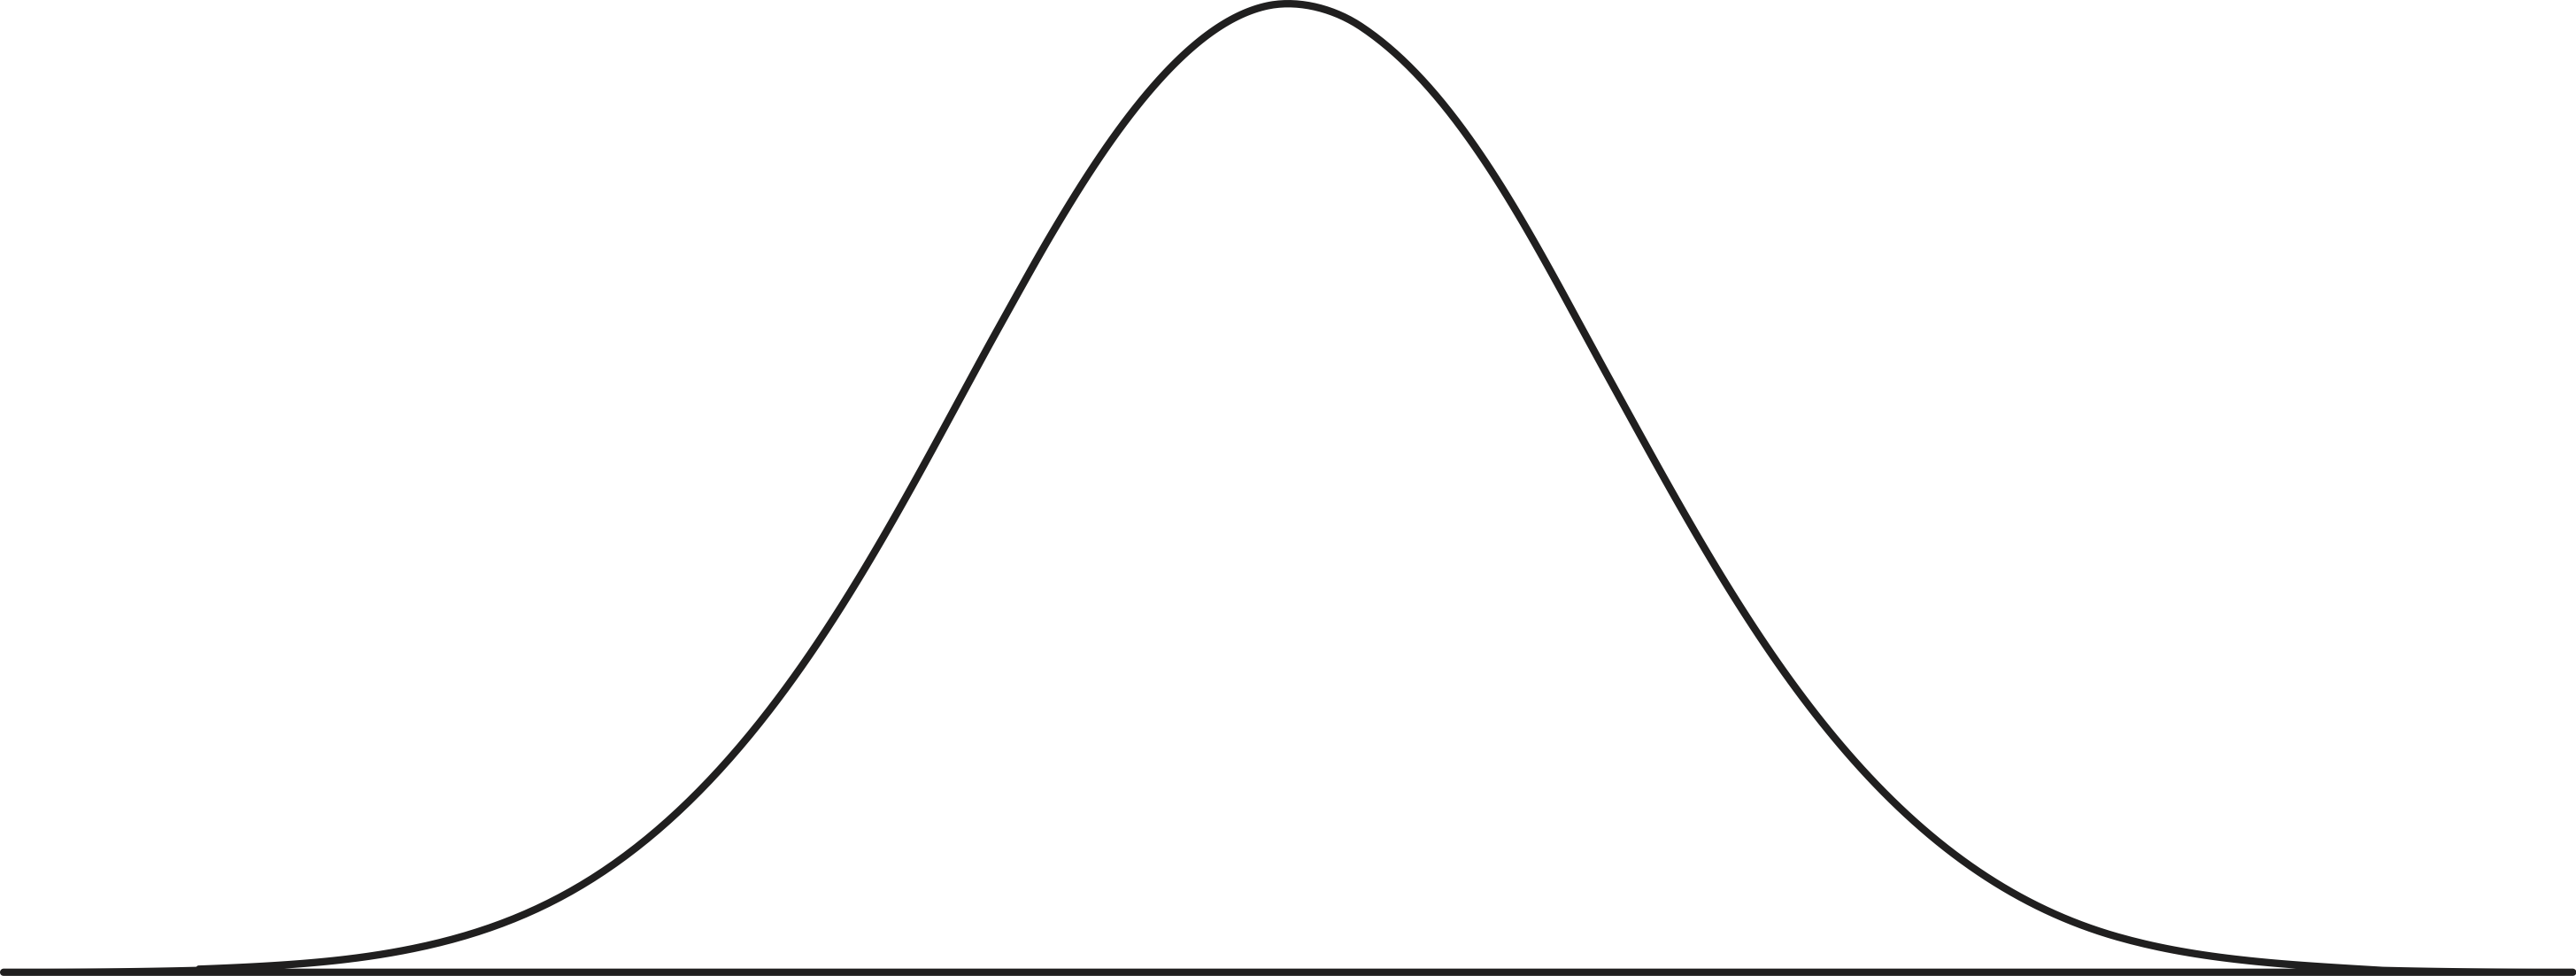
\includegraphics[width=1\textwidth]{stats1.png}
    \end{minipage}
    \begin{minipage}{0.79\textwidth}
    	\begin{tabular}{ll}
            выборка:                        & $X^n=\left(X_1,\ldots,X_n\right), \; X \sim \prob \in \Omega$         \\
            нулевая гипотеза:               & $H_0\colon \prob\in\omega, \;\; \omega\in\Omega$ \\
            альтернативная гипотеза         & $H_1\colon \prob\notin\omega$ \\
            статистика:                     & $T\left(X^n\right), \;\; T\left(X^n\right)\sim F\left(x\right) \;\text{при}\; \prob\in\omega$ \\
            & \;\;\;\;\;\;\;\;\;\;\;\;\;\; $T\left(X^n\right)\not\sim F\left(x\right) \;\text{при}\; \prob\notin\omega$ \\
        \end{tabular}
    \end{minipage}

    \bigskip

    \begin{minipage}{0.20\textwidth}
        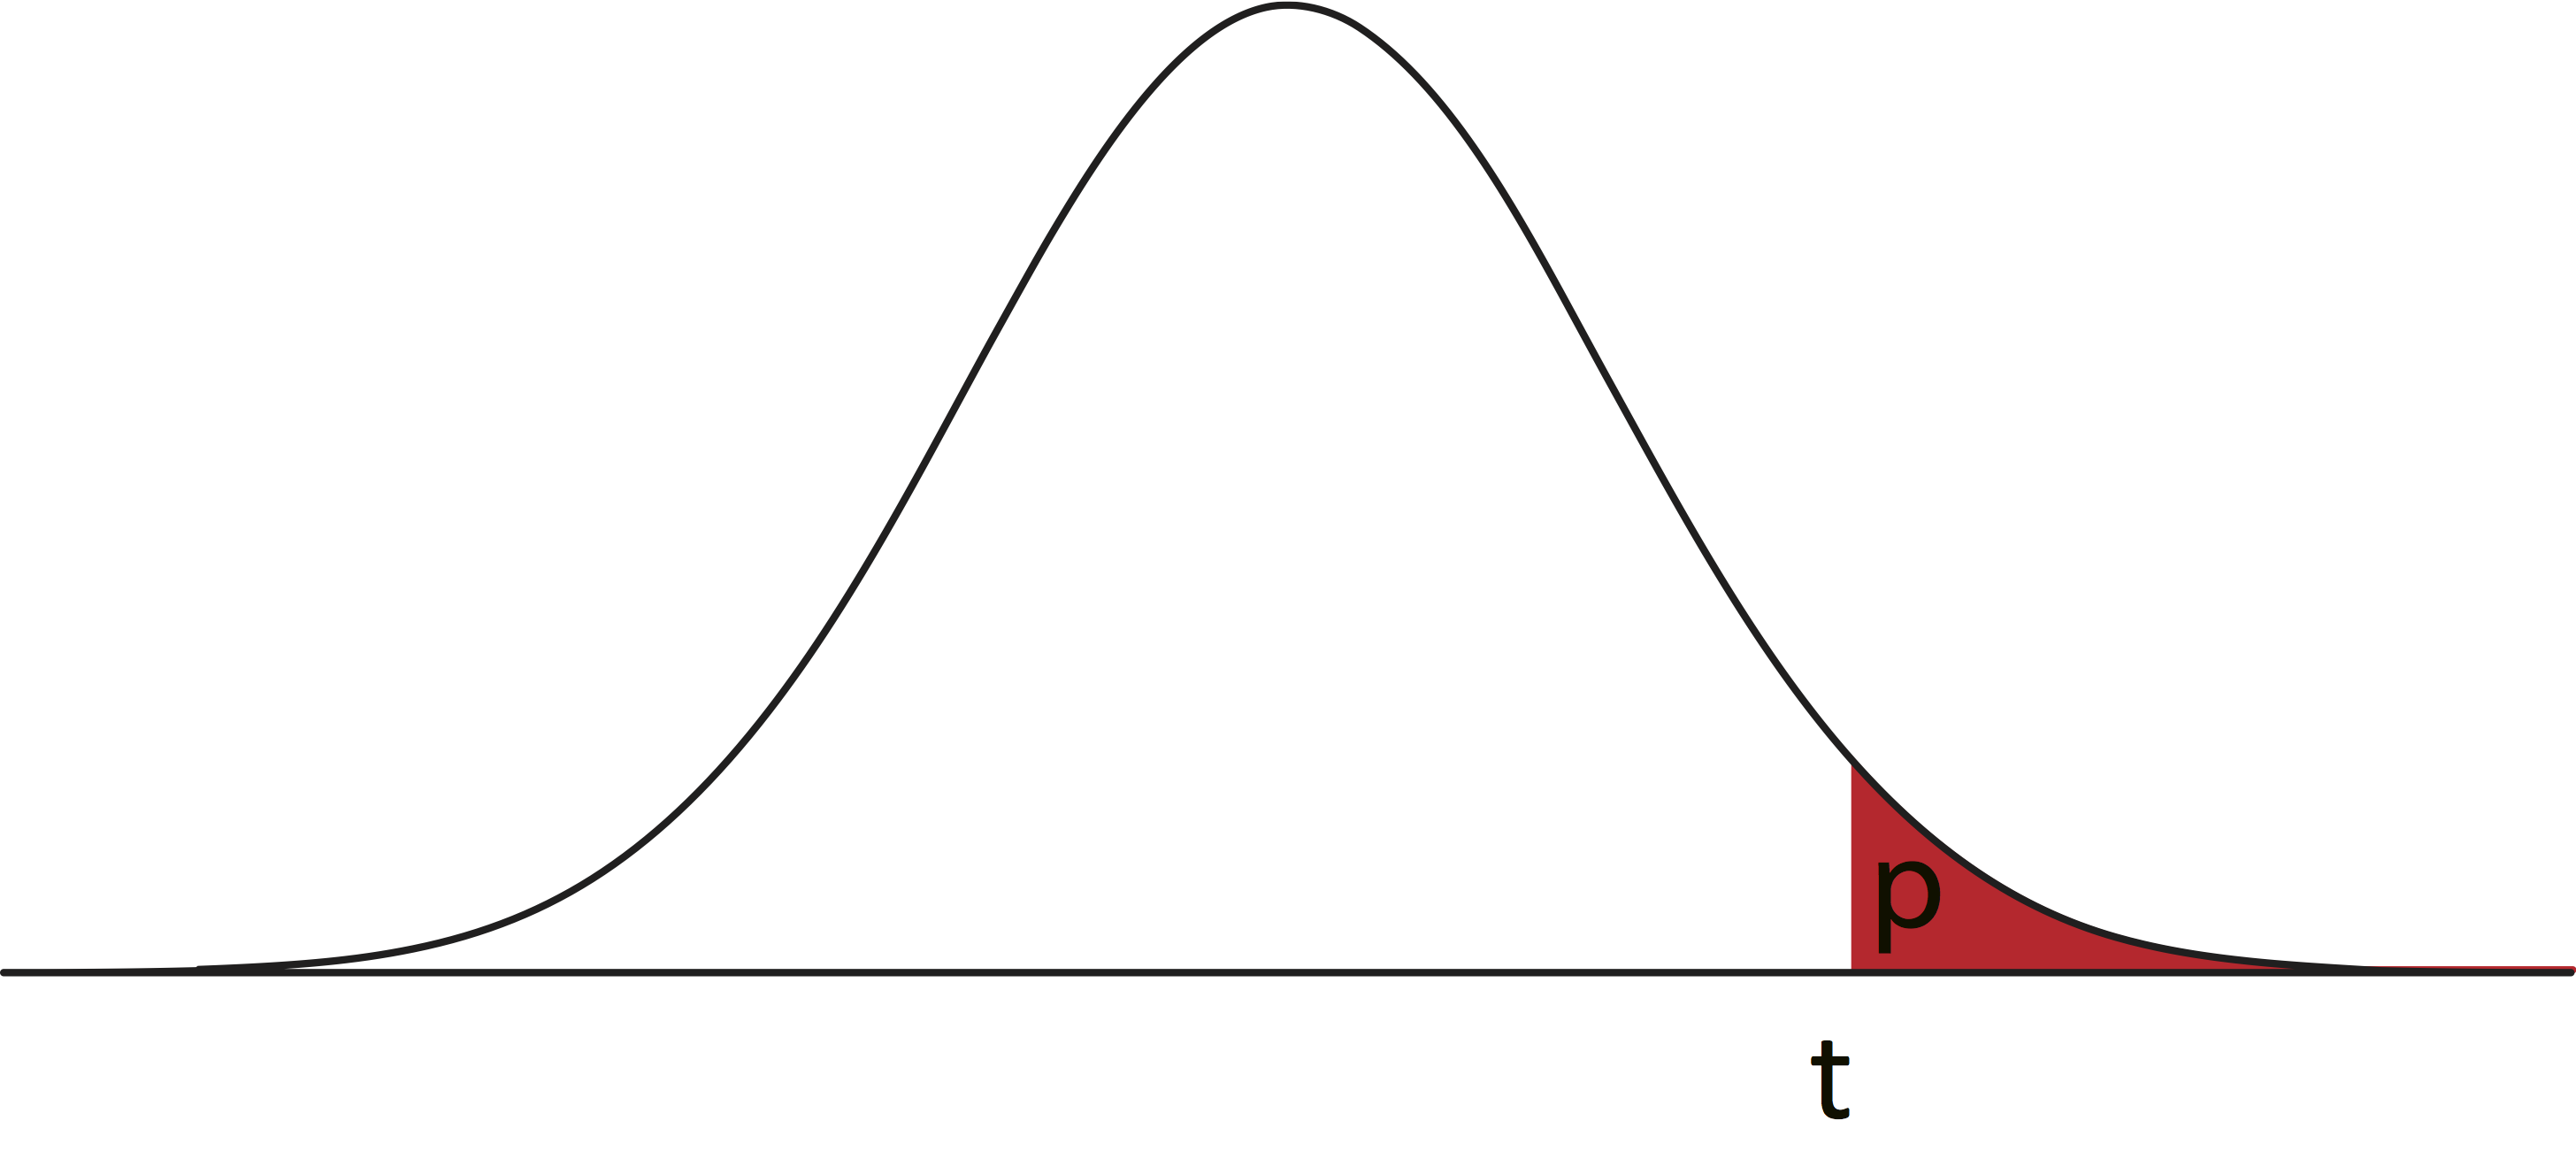
\includegraphics[width=1\textwidth]{stats2.png}
    \end{minipage}
    \begin{minipage}{0.79\textwidth}
        \begin{tabular}{ll}
    	   Реализация выборки:             & $x^n=\left(x_1,\ldots,x_n\right)$ \\
            Наблюдаемая статистика:          & $t = T \left(x^n\right)$ \\
            Достигаемый уровень значимости:
            & $p\left(x^n\right)$~--- вероятность при $H_0$\\
            & получить $T \left(X^n\right)=t$\\
            & или более экстремальное\\
        \end{tabular}
    \end{minipage}

    \begin{center}

    \begin{tabular}{ll}
        \multicolumn{2}{c}{ $p\left(x^n\right) = \prob\left(T\geqslant  t\left|H_0\right.\right)$ } \\
        \multicolumn{2}{c}{Гипотеза отвергается при $p\left(x^n\right)\leqslant\alpha,\;\;\alpha$~--- уровень значимости} \\    \end{tabular}
    \end{center}
\end{frame}
%%%%%%%%%%%%%%%%%%%%%%%%%%%%%%%%%%%%%%%%%%%%%%%%%%%%%%%%%%%%%%%%%%%%%%%
% Достигаемый уровень значимости - достаточно сложная концепция. Например, авторы блога fivethirtyeight на конференции по мета-анализу провели опрос участников, спрашивая их, что такое достигаемый уровень значимости, и получили набор ответов от неправильных до "я не помню, нужно спросить моего аспиранта". И это исследователи - люди, которые часто сталкиваются со статистикой!
% Проблема определения p-value в том, что оно длинное, но из него ничего нельзя выбросить так, чтобы оно не стало неправильным. Например, часто хочется думать, что p-value — это просто вероятность справедливости нулевой гипотезы, но это не так! Это хорошо понятно на следующем примере. В 2010 году осьминог Поль угадывал результаты матчей чемпионата мира по футболу с участием сборной Германии, выбирая из двух кормушек ту, на которой был изображён флаг страны-победителя. Из 13 матчей, в которых он пробовал свои силы, результаты 11 ему удалось угадать. Используя эти данные как выборку, можно проверить нулевую гипотезу о том, что он выбирал кормушку наугад против альтернативы о том, у осьминога есть сверхспособности к предсказанию результатов матчей. Критерий, которым проверяется эта нулевая гипотеза, будет разобран позже. Но если его применить, получится достигаемый уровень значимости p = 0.0112. Это значение — не вероятность, что осьминог выбирает кормушку наугад. Вероятность того, что осьминог выбирает кормушку наугад, равна единице! p = 0.0112 — это именно вероятность получить такие или ещё более экстремальные данные при условии справедливости нулевой гипотезы. Эта вероятность достаточно мала, но редкие события тоже происходят. И, как правило, именно о них пишут в газетах.
%%%%%%%%%%%%%%%%%%%%%%%%%%%%%%%%%%%%%%%%%%%%%%%%%%%%%%%%%%%%%%%%%%%%%%%

\begin{frame}{Ошибки I и II рода}{матрица ошибок}
%%%%%%%%%%%%%%%%%%%%%%%%%%%%%%%%%%%%%%%%%%%%%%%%%%%%%%%%%%%%%%%%%%%%%%%
% Существенная особенность механизма проверки гипотез — его несимметричность относительно пары нулевая гипотеза – альтернатива.
%Эта особенность тесно связана с понятиями ошибок первого и второго рода.
%Нулевая гипотеза может быть либо верна, либо неверна.
%В результате проверки гипотезы ее: можно либо принять, либо отвергнуть.
%На главной диагонали находятся верные решения: либо принимается верная нулевая гипотеза, либо отвергается неверная нулевая гипотеза.
%А вот на побочной диагонали располагаются ошибки.
%Совершить ошибку первого рода — значит отвергнуть верную нулевую гипотезу.
%Если же принимается неверная нулевая гипотеза, то это ошибка второго рода.
%%%%%%%%%%%%%%%%%%%%%%%%%%%%%%%%%%%%%%%%%%%%%%%%%%%%%%%%%%%%%%%%%%%%%%%

	\begin{center}
    \begin{tabular}{ |r | >{\centering}p{5.5cm} | >{\centering}p{5.5cm} | }
        \hline
        & $H_0$ верна         & $H_0$ неверна \tabularnewline \hline
        $H_0$ принимается & 
\includegraphics[height=2.5cm]{TP.png}
        \newline верно принята
        & 
\includegraphics[height=2.5cm]{FN.png}
        \newline Ошибка II рода (False negative)
        \tabularnewline \hline
        $H_0$ отвергается & 
\includegraphics[height=2.5cm]{FP.png}
        \newline Ошибка I рода (False positive) & 
\includegraphics[height=2.5cm]{TN.png}$H_0$
        \newline верно отвергнута
         \tabularnewline
        \hline
    \end{tabular}
    \end{center}

\end{frame}
\begin{frame}{Ошибки I и II рода}{Свойства ошибок}
%%%%%%%%%%%%%%%%%%%%%%%%%%%%%%%%%%%%%%%%%%%%%%%%%%%%%%%%%%%%%%%%%%%%%%%
% В механизме проверки гипотез ошибки первого и второго рода неравнозначны.
%Ошибка первого рода критичнее, вероятность отвержение нулевой гипотезы в случае, когда она верна, жестко ограничивается.
%Если нулевая гипотеза отвергается при значении уровня значимости $$p \leqslant \alpha$, то вероятность ошибки первого рода получается ограниченной сверху величиной $\alpha$.
%Таким образом, любой корректный критерий имеет вероятность ошибки первого рода не больше, чем уровень значимости.
%Что касается ошибки второго рода, то она минимизируется.
%
%Понятие ошибки второго рода связано с понятием мощности статистического критерия.
%
%Мощность — это вероятность отвергнуть неверную нулевую гипотезу.
%Чтобы найти идеальный критерий для проверки пары нулевая гипотеза – альтернатива, нужно среди всех корректных критериев выбрать критерий с максимальной мощностью.
%%%%%%%%%%%%%%%%%%%%%%%%%%%%%%%%%%%%%%%%%%%%%%%%%%%%%%%%%%%%%%%%%%%%%%%
	Задача проверки гипотез несимметрична относительно пары $\left(H_0,H_1\right)$: вероятность ошибки первого рода ограничивается сверху величиной $\alpha$, а второго рода~--- минимизируется путём выбора критерия.

	\bigskip
    \begin{itemize}
	\item \structure{Корректный} критерий: $\prob\left(p\left(T\right)\leqslant\alpha\left|H_0\right.\right)\leqslant  \alpha$ $\forall \prob \in \Omega$.

	\item \structure{Мощность}: $\pow = \prob\left(p\left(T\right)\leqslant\alpha\left|H_1\right.\right).$

    \item \structure{Состоятельный} критерий: $\pow \rightarrow 1 $ для всех альтернатив $H_1$ при $n\rightarrow \infty$.

    \item $T_1$~--- \structure{равномерно наиболее мощный} критерий, если $\forall T_2$
	\begin{align*}
	\prob\left(p\left(T_1\right)\leqslant  \alpha\left|H_1\right.\right) & \geqslant  \prob\left(p\left(T_2\right)\leqslant  \alpha\left|H_1\right.\right) \;\; \forall H_1\neq H_0, \\
	\prob\left(p\left(T_1\right)\leqslant  \alpha\left|H_0\right.\right) & = \prob\left(p\left(T_2\right)\leqslant  \alpha\left|H_0\right.\right),
	\end{align*}
	причём хотя бы для одной $H_1$ неравенство строгое.
    \end{itemize}
\end{frame}


%
%\begin{frame}{Матрица ошибок}{}
%    \begin{tabular}{|>{\columncolor{blue}}l|m{35mm}|m{35mm}|}
%        \hline
%        \rowcolor{blue}& $\color{white} H_0$ \color{white}  верна & $\color{white} H_0$ \color{white} неверна\\
%        \hline
%        $\color{white} H_0$ \color{white} принята & Верное решение &  \cellcolor{red!30} Ошибка II рода \\
%        \hline
%        $\color{white} H_0$ \color{white} отвергнута & \cellcolor{red!30}  Ошибка I рода &  Верное решение\\
%        \hline
%    \end{tabular}
%
%    \vfill
%    \begin{itemize}
%        \item \alert{Ошибка первого рода}~--- отвержение верной гипотезы $H_0$.
%        \item \alert{Ошибка второго рода}~--- принятие ошибочной гипотезы $H_0$.
%    \end{itemize}
%
%    \vfill
%
%    % Какая из ошибок является более опасной, зависит от конкретной задачи.
%
%    \vfill
%    {\centering
%        \begin{tikzpicture}
%            \begin{axis}[
%                name=myaxis,
%                no markers, domain=-2:4, samples=500,
%                axis y line=none,
%                axis x line=center,
%                xlabel=$T$, %ylabel=$p$,
%                every axis y label/.style={at=(current axis.above origin),anchor=south},
%                every axis x label/.style={at=(current axis.right of origin),anchor=west},
%                height=5cm, width=11cm,
%                xmin=-2.1, xmax=4.1,
%                ymin=-0.1, ymax=0.5,
%                xtick=\empty, ytick=\empty,
%                enlargelimits=false, clip=false, axis on top,
%                grid = none
%                ]
%                \addplot [fill=cyan!20, draw=none, domain=1.4:3] {gauss(0,1)} \closedcycle;
%                \addplot [fill=red!20, draw=none, domain=0:1.4] {gauss(3,1)} \closedcycle;
%                \addplot [very thick,cyan!50!black] {gauss(0,1)};
%                \addplot [very thick,red!50!black] {gauss(3,1)};
%
%                \draw[thick,red!50, rounded corners = 4mm] (axis cs:4,-0.05) -| (axis cs:1.4,0);
%                \draw[thick,cyan!50, rounded corners = 4mm] (axis cs:-2,-0.05) -| (axis cs:1.4,0);
%
%                % \fill[cyan!20] (axis cs:1.4,-0.02) rectangle (axis cs:-2,0);
%
%                \node[coordinate,pin=135:{Ошибка II рода}]
%                at (axis cs:1.2,0.02) {};
%                \node[coordinate,pin=45:{Ошибка I рода}]
%                at (axis cs:1.6,0.04) {};
%                \draw[red] (axis cs:1.4,-0.04) node[below]{$T_\text{кр.}$} -- (axis cs:1.4,0.5);
%            \end{axis}
%        \end{tikzpicture}
%        \par}
%\end{frame}

\begin{frame}{Интерпретация результата Absence of evidence $\nRightarrow$ evidence of absence.}
%%%%%%%%%%%%%%%%%%%%%%%%%%%%%%%%%%%%%%%%%%%%%%%%%%%%%%%%%%%%%%%%%%%%%%%
% Неравнозначность нулевой и альтернативной гипотезы видна уже на уровне терминологии.
%Если достигаемый уровень значимости p <= alpha, то говорят, что нулевая гипотеза отвергается в пользу альтернативы.
%Если достигаемый уровень значимости p > alpha, то нулевая гипотеза не отвергается.
%
%Когда гипотеза не отвергается, это значит только то, что нет доказательств того что она неверна.
%Но отсутствие доказательств не является доказательством ее верности!
%Это можно лучше понять на примере судебного процесса.
%Презумпции невиновности: подсудимый по умолчанию невиновен (это нулевая гипотеза), и, если доказательств обратному нет, нельзя утверждать, что он преступник, даже если он на самом деле совершил преступление.
%%%%%%%%%%%%%%%%%%%%%%%%%%%%%%%%%%%%%%%%%%%%%%%%%%%%%%%%%%%%%%%%%%%%%%%
    \begin{itemize}
	\item Если величина~$p$ достаточно мала, то данные свидетельствуют против нулевой гипотезы в пользу альтернативы\hfill \alert{Гипотезу $H_0$ можно отвергнуть}

	\item Если величина $p$ недостаточно мала, то данные не свидетельствуют против нулевой гипотезы в пользу альтернативы. \hfill \alert{Нет причин отвергать гипотезу~$H_0$}
    \end{itemize}
	\bigskip

    \centering
	При помощи инструмента проверки гипотез нельзя доказать справедливость нулевой гипотезы!


\end{frame}

\begin{frame}{Статистическая и практическая значимость}{}
%%%%%%%%%%%%%%%%%%%%%%%%%%%%%%%%%%%%%%%%%%%%%%%%%%%%%%%%%%%%%%%%%%%%%%%
% На самом деле эксперименты проводятся не для того, чтобы получить значение p-value.
%Как правило, исследователя интересует размер эффекта, то есть степень отклонения данных от нулевой гипотезы.
%Например, если эксперимент связан с проверкой способностей предсказателя будущего, то размер эффекта — это вероятность верного предсказания.
%Если проверяется эффективность лекарства, то размер эффекта — это вероятность выздоровления пациента, который это лекарство принимает, за вычетом эффекта плацебо.
%При запуске программы лояльности для пользователей интернет-магазина размер эффекта — это последующее увеличение среднего чека.
%
% Размер эффекта — это величина, определенная на генеральной совокупности.
%Но, как правило, у исследователя есть только небольшая выборка из нее, а оценка размера эффекта по выборке — это случайная величина.
%Маленький достигаемый уровень значимости является показателем того, что такую оценку размера эффекта, какая получена по выборке, с маленькой вероятностью можно было получить случайно.
%Достигаемый уровень значимости зависит не только от размера эффекта, но и от объема выборки, по которой оценивается эффект.
%
%Если выборка небольшая, скорее всего, нулевая гипотеза на ней не отвергается (если только она не слишком дикая).
% Однако с ростом объема выборки начинают проявляться все более тонкие отклонения данных от нулевой гипотезы.
%На достаточно большой выборке велика вероятность, что значительная часть разумных нулевых гипотез будет отвергнута.
%Именно поэтому, даже если нулевая гипотеза отвергнута, это еще не значит, что полученный эффект имеет какую-то практическую значимость, её нужно оценивать отдельно.
%%%%%%%%%%%%%%%%%%%%%%%%%%%%%%%%%%%%%%%%%%%%%%%%%%%%%%%%%%%%%%%%%%%%%%%
    \begin{itemize}
	   \item Выбранная статистика может отражать не всю информацию, содержащуюся в выборке:
        \begin{gather*}
            H_0\colon X\sim N\left(\mu, \sigma^2\right), \qquad
            H_1\colon \not\sim N\left(\mu, \sigma^2\right)
            \\
            T\left(X^n\right)= \Skew(X^n).
        \end{gather*}
Все симметричные распределения будут признаны нормальными!
		\item Вероятность отвергнуть нулевую гипотезу зависит не только от того, насколько она отличается от истины, но и от размера выборки.

		\item По мере увеличения $n$ могут выявиться более тонкие несоответствия выборки гипотезе~$H_0$, и она будет отвергнута.
    \end{itemize}

	\bigskip

	\alert{При любой проверке гипотез нужно:}
    \begin{itemize}
        \item оценивать \structure{размер эффекта}~--- степень отличия нулевой гипотезы отличается от истины,
        \item оценивать его практическую значимость.
    \end{itemize}
\end{frame}
\begin{frame}{Статистическая и практическая значимость}{Примеры}
%%%%%%%%%%%%%%%%%%%%%%%%%%%%%%%%%%%%%%%%%%%%%%%%%%%%%%%%%%%%%%%%%%%%%%%
% Первый пример связан с большим исследованием, в рамках которого на протяжении трех лет у большой выборки женщин измеряли вес, а также оценивали, насколько активно они занимаются спортом.
% По итогам исследования выяснилось, что женщины, которые в течение этого времени упражнялись не меньше часа в день, набрали значительно меньше веса, чем женщины, которые упражнялись менее 20 минут в день.
%Статистическая значимость этого результата достаточно высока: p < 0.001.
%Проблема в размере эффекта: разница в набранном весе между двумя исследуемыми группами женщин составила всего 150 граммов.
%150 граммов за 3 года — это не очень много.
%Крайне сомнительно, что этот эффект имеет какую-то практическую значимость.
%Еще один пример связан с клиническими испытаниями гормонального препарата «Премарин», который облегчает симптомы менопаузы. В 2002 году эти испытания были прерваны досрочно, поскольку было обна- ружено, что прием препарата ведет к значимому увеличению риска развития рака груди (на 0.08%), инсульта (на 0.08%) и инфаркта (на 0.07%). Этот эффект статистически значим; при этом на первый взгляд кажется, что размеры эффектов ничтожны. Например, если кому-то сказать, что его любимые конфеты повышают риск возникновения инфаркта на 0.07%, вряд ли это заставит человека отказаться от этих конфет. Тем не менее, если пересчитать размеры эффектов на всю популяцию людей, которым этот препарат может быть по- тенциально приписан, результатом будут тысячи дополнительных смертей. Разработчики препарата не могут взять на себя эту ответственность, поэтому такой препарат немедленно запрещают и снимают с рынка.
% Этот пример показывает, что практическую значимость результата нельзя определить на глаз. В идеале она должна определяться человеком, который поставил задачу и понимает предметную область.
% Еще один пример — это испытание лекарства, которое замедляет ослабление интеллекта у людей, страдающих болезнью Альцгеймера.
%В этом исследовании очень сложно измерить размер эффекта.
%В течение эксперимента одна часть испытуемых должна принимать лекарство, а другая — плацебо.
%Только по прошествии нескольких лет можно будет сравнить эти две группы.
%Поэтому такое исследование длится долгое время и дорого стоит.
%Если при испытании оказывается, что разница между снижением IQ в контрольной группе, где люди принимали плацебо, и тестовой группе, где люди принимали препарат, составляет 13 пунктов, это различие очень большое, и на практике этот эффект крайне значим.
%При этом может оказаться, что статистическая значимость не была достигнута, то есть $p > alpha$, и формально нулевую гипотезу об отсутствии эффекта лекарства нельзя отвергнуть.
%Если предмет исследования очень важен, то, оказавшись в подобной ситуации, возможно, стоит продолжать исследования: набрать еще выборку, уменьшить дисперсию оценки размера эффекта и убедиться в том, что важное открытие не упущено.
%%%%%%%%%%%%%%%%%%%%%%%%%%%%%%%%%%%%%%%%%%%%%%%%%%%%%%%%%%%%%%%%%%%%%%%
	\begin{itemize}
		\item За 3~года женщины, упражнявшиеся не меньше 1~часа в день, набрали значимо меньше веса, чем женщины, упражнявшиеся меньше 20~минут в день ($p<0.001$). \hfill (\textit{Lee et al, 2010})
        \begin{itemize}
            \item Разница в~набранном весе составила 150~г.
		    \item Практическая значимость такого эффекта сомнительна.
        \end{itemize}

		\item В 2002 году клинические испытания гормонального препарата Премарин были досрочно прерваны. \hfill (\textit{Ellis, 2010, гл.~2})
        \begin{itemize}
            \item обнаружено, что его приём ведёт к~значимому увеличению риска развития рака груди на~0.08\%, риска инсульта на~0.08\% и~инфаркта на~0.07\%.
        \end{itemize}

		\item если при испытании гипотетического лекарства, позволяющего замедлить прогресс ослабления интеллекта больных Альцгеймером, оказывается, что разница в IQ контрольной и тестовой групп составляет 13~пунктов, возможно, изучение лекарства стоит продолжить, даже если эта разница статистически незначима.\hfill (\textit{Kirk, 1996})
	\end{itemize}
\end{frame}


\begin{frame}{Гипотезы о числовых характеристиках}

    Гипотезы вида $H_0\colon \theta=\theta_0$ можно проверять при помощи доверительных интервалов для $\theta$:
    \begin{itemize}
        \item если $\theta_0$ не попадает в $(1-\alpha)$ доверительный интервал для $\theta$, то $H_0$ отвергается на уровне значимости~$\alpha$;
        \item p-value~--- максимальное $\alpha$, при котором $\theta_0$ попадает в~соответствующий доверительный интервал.
    \end{itemize}
\end{frame}

\subsection{Пример}
\begin{frame}{Пример: Shaken, not stirred}
%%%%%%%%%%%%%%%%%%%%%%%%%%%%%%%%%%%%%%%%%%%%%%%%%%%%%%%%%%%%%%%%%%%%%%%
%
%%%%%%%%%%%%%%%%%%%%%%%%%%%%%%%%%%%%%%%%%%%%%%%%%%%%%%%%%%%%%%%%%%%%%%%
	Джеймс Бонд говорит, что предпочитает мартини взболтанным, но не смешанным.

    \begin{itemize}
    \item Проведём слепой тест: $n$ раз предложим ему пару напитков и~выясним, какой из двух он предпочитает.

	\item \structure{Выборка:} бинарный вектор длины $n$, $1$~--- Джеймс Бонд предпочёт взболтанный, $0$~--- смешанный.


	\item \structure{Нулевая гипотеза:} Джеймс Бонд не различает два вида мартини.

	\bigskip

	\item \structure{Статистика $T$}~--- число единиц в выборке.
    \end{itemize}
\end{frame}

\begin{frame}{Нулевое распределение}

	Если нулевая гипотеза справедлива, то равновероятны все выборки длины $n$ из нулей и единиц.

	\bigskip

	Пусть $n=16$, тогда существует $2^{16} = 65536$ равновероятных варианта. Статистика $T$ принимает значения от $0$ до $16$:

	\begin{center}
		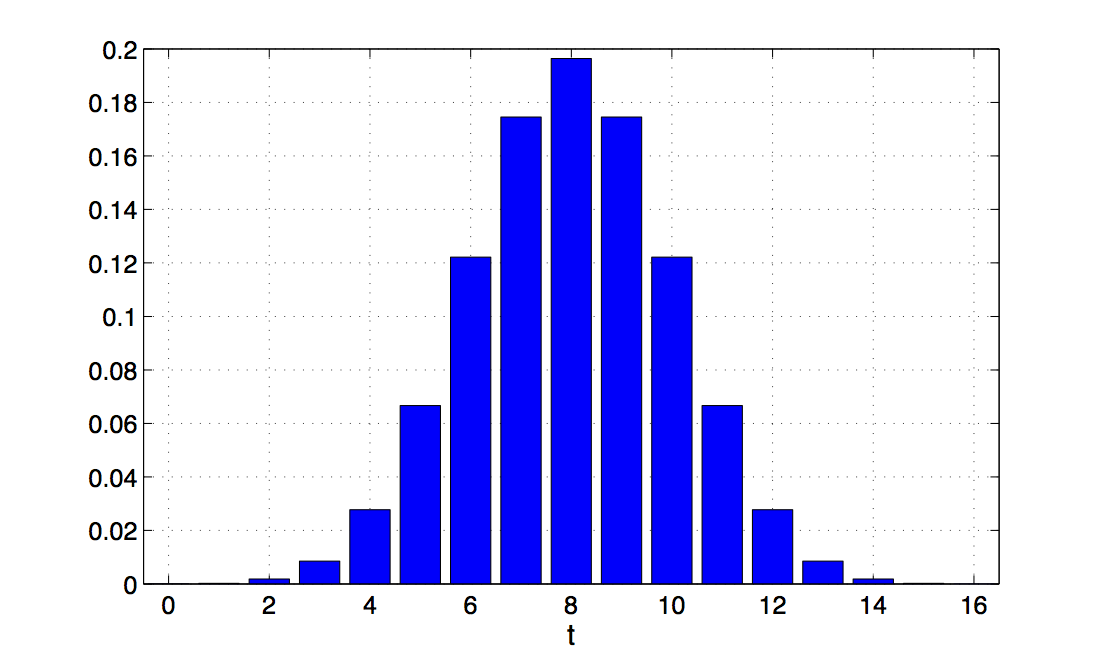
\includegraphics[height=0.5\textheight]{bond1.png}
	\end{center}

\end{frame}

\begin{frame}{Односторонняя альтернатива}
%%%%%%%%%%%%%%%%%%%%%%%%%%%%%%%%%%%%%%%%%%%%%%%%%%%%%%%%%%%%%%%%%%%%%%%
% достигаемый уровень значимости здесь - это суммарная высота всех красных столбиков
%%%%%%%%%%%%%%%%%%%%%%%%%%%%%%%%%%%%%%%%%%%%%%%%%%%%%%%%%%%%%%%%%%%%%%%
	\alert{$H_1\colon$ Джеймс Бонд предпочитает взболтанный мартини.}

    \medskip
	При справедливости такой альтернативы более вероятны большие значения $T$ (большие значения~$T$ свидетельствуют против $H_0$ в пользу $H_1$).

    \medskip
	Вероятность того, что Джеймс Бонд предпочтёт взболтанный мартини в $12$-и или более случаях из $16$ при справедливости $H_0$, равна $\frac{2517}{65536}\approx 0.0384$.

    \begin{center}
		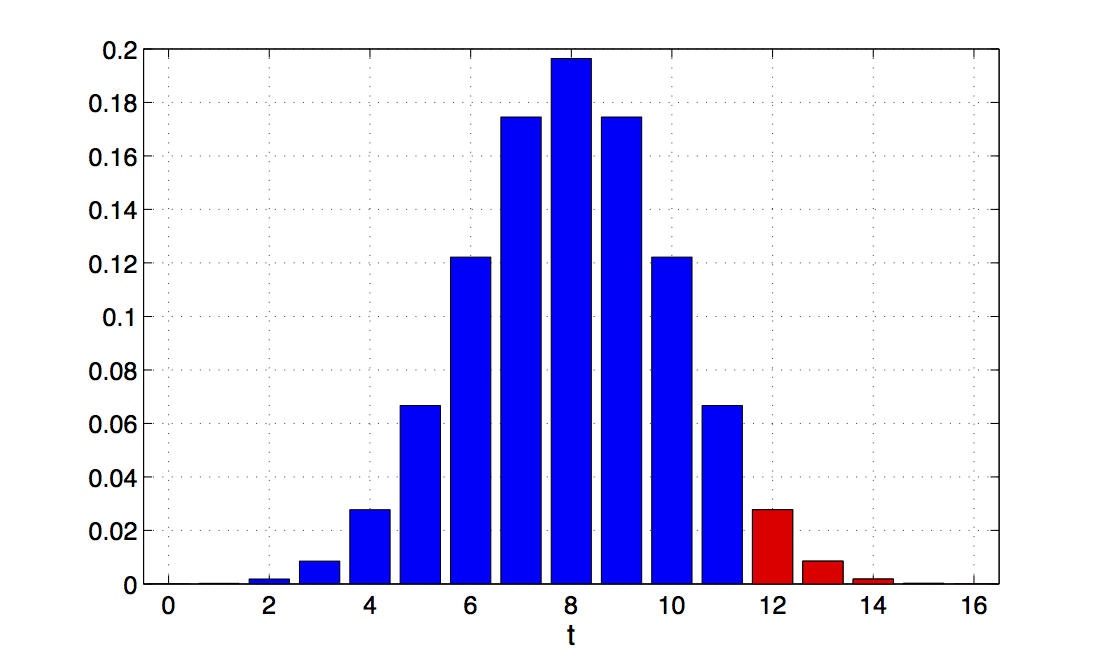
\includegraphics[height=0.5\textheight]{bond2.png}
	\end{center}
	$0.0384$~--- достигаемый уровень значимости при реализации $t=12$.
\end{frame}

\begin{frame}{Двусторонняя альтернатива}

    \alert{$H_1\colon$ Джеймс Бонд предпочитает какой-то определённый вид мартини.}

    \medskip

	При справедливости такой альтернативы и большие, и маленькие значения~$T$ свидетельствуют против $H_0$ в пользу $H_1$).

    \medskip

	Вероятность того, что Джеймс Бонд предпочтёт взболтанный мартини в~$\geqslant  12$ случаях из $16$ при справедливости $H_0$, равна $\frac{5034}{65536}\approx 0.0768$.

	\begin{center}
		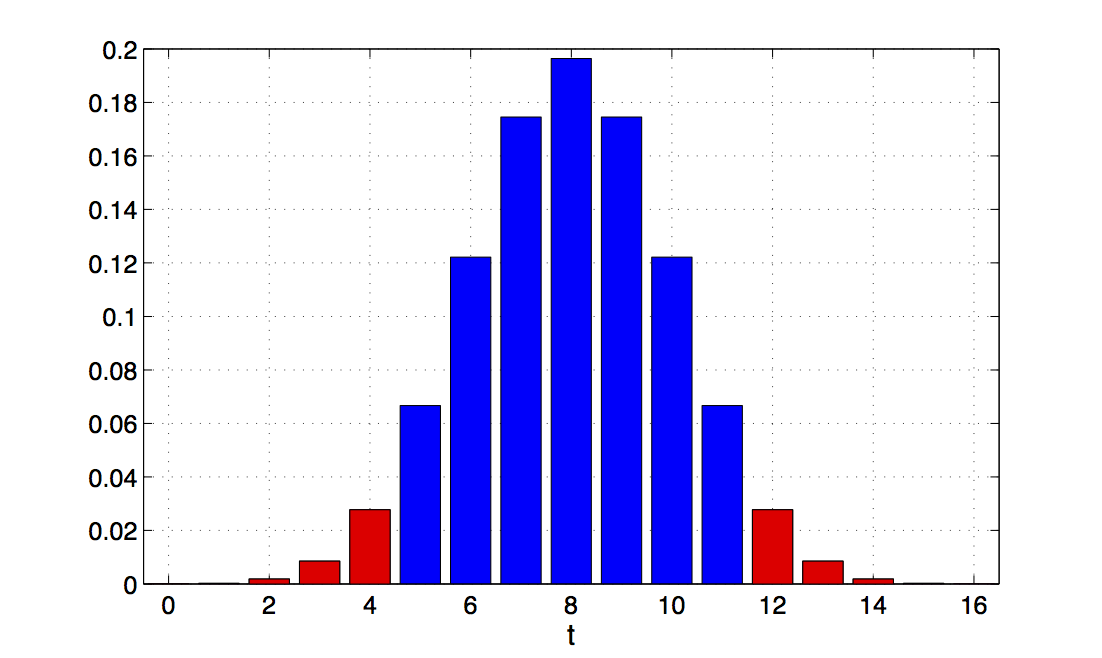
\includegraphics[height=0.5\textheight]{bond3.png}
	\end{center}
	$0.0768$~--- достигаемый уровень значимости при реализации $t=12$.
\end{frame}

\begin{frame}{Достигаемый уровень значимости}
%%%%%%%%%%%%%%%%%%%%%%%%%%%%%%%%%%%%%%%%%%%%%%%%%%%%%%%%%%%%%%%%%%%%%%%
%
%%%%%%%%%%%%%%%%%%%%%%%%%%%%%%%%%%%%%%%%%%%%%%%%%%%%%%%%%%%%%%%%%%%%%%%
		Чем ниже достигаемый уровень значимости, тем сильнее данные свидетельствуют против нулевой гипотезы в пользу альтернативы.

		\bigskip

		$0.0384$~--- вероятность реализации $t\geqslant  12$ при условии, что нулевая гипотеза справедлива, т.\,е. Джеймс Бонд выбирает мартини наугад.

%		\bigskip
%
%		Ещё раз: это не вероятность справедливости нулевой гипотезы!

    \bigskip

		\structure{Пример:} Допустим Джеймс Бонд выбирает взболтанный мартини в $51$\% случаев.

		Однако, по итогам $100$ испытаний взболтанный мартини был выбран $49$ раз.

		\bigskip

        Достигаемый уровень значимости против односторонней альтернативы~--- $p\approx 0.6178.$

        \bigskip

        Нулевая гипотеза не отвергается.

%        При этом сказать, что она верна, было бы ошибкой~--- Джеймс Бонд выбирает смешанный и взболтанный мартини не с одинаковыми вероятностями!
\end{frame}

\begin{frame}{Мощность}
%%%%%%%%%%%%%%%%%%%%%%%%%%%%%%%%%%%%%%%%%%%%%%%%%%%%%%%%%%%%%%%%%%%%%%%
% Предполагая значение параметра, относительно которого мы проверяем гипотезу, известным, мы можем построить распределение значений статистики при этом значении. Чтобы получить мощность, нужно просуммировать высоты всех столбиков, соответствующих значениям статистики, при которых нулевая гипотеза отвергается.
%%%%%%%%%%%%%%%%%%%%%%%%%%%%%%%%%%%%%%%%%%%%%%%%%%%%%%%%%%%%%%%%%%%%%%%
	\only<1>{
		Проверяя нулевую гипотезу против двусторонней альтернативы, мы отвергаем $H_0$ при $t\geqslant  13$ или $t \leqslant  3$, что обеспечивает достигаемый уровень значимости $p=0.0213\leq\alpha=0.05$.
		\begin{center}
			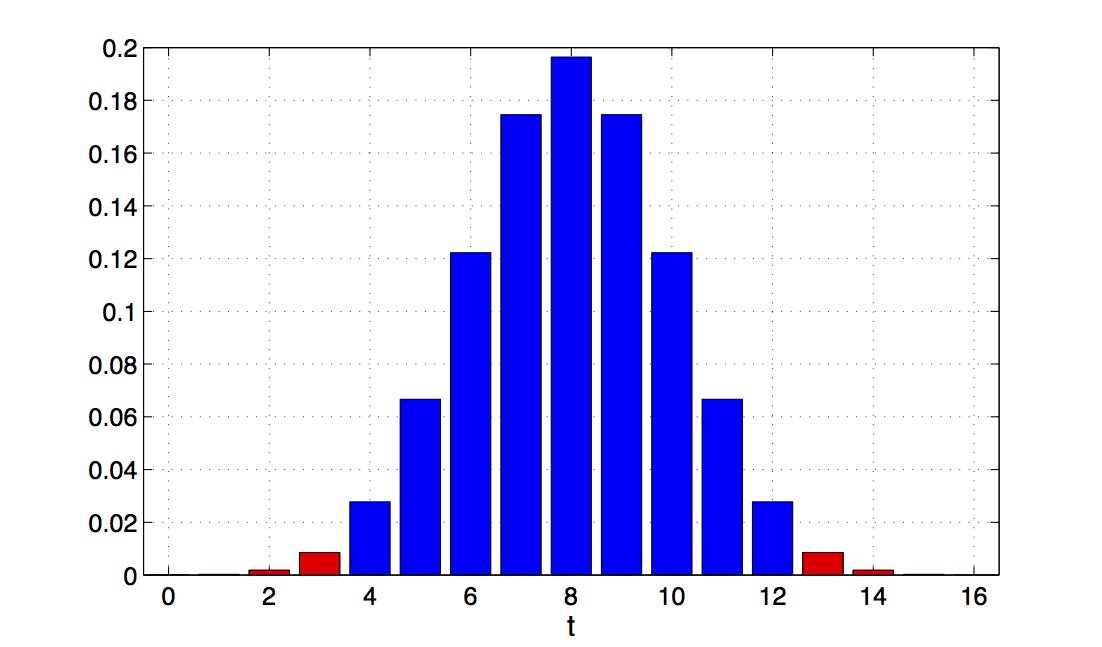
\includegraphics[height=0.3\textheight]{bond5.png}
		\end{center}
		Пусть Джеймс Бонд выбирает взболтанный мартини в $75$\% случаев.%    \vspace{-5pt}
		\begin{center}
			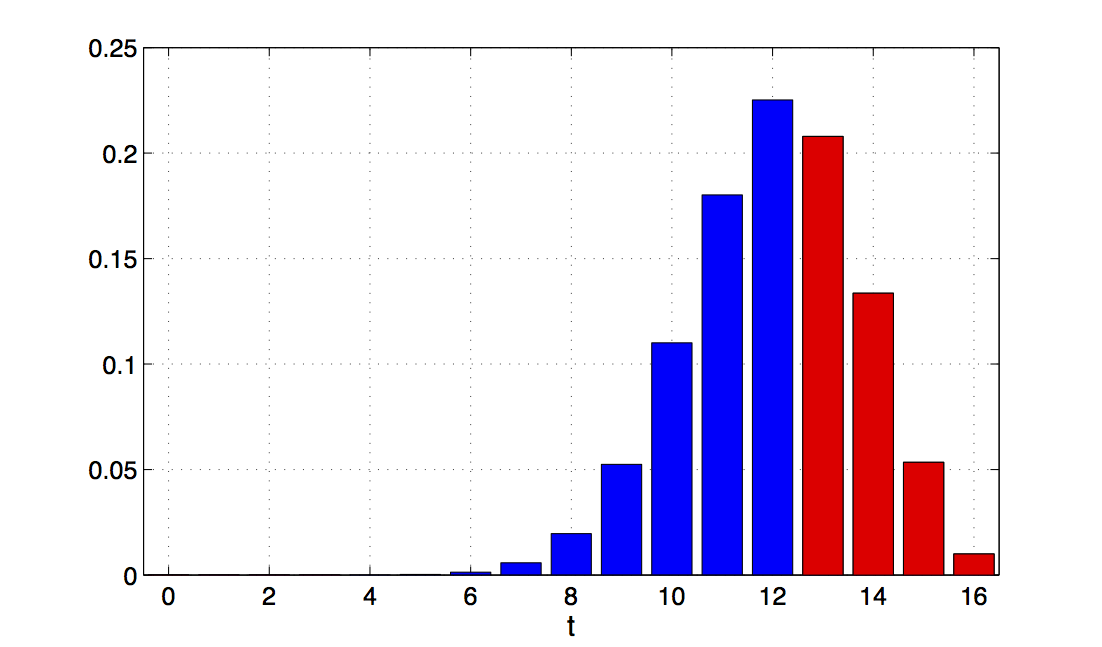
\includegraphics[height=0.3\textheight]{bond6.png}
		\end{center}
		$\pow \approx 0.6202,$ т.\,е., при многократном повторении эксперимента гипотеза будет отклонена только в $62$\% случаев.
	}

\only<2>{
	Мощность критерия зависит от следующих факторов:
	\begin{itemize}
		\item размер выборки
		\item размер отклонения от нулевой гипотезы
		\item чувствительность статистики критерия
		\item тип альтернативы
	\end{itemize}
}

	\only<3>{
%%%%%%%%%%%%%%%%%%%%%%%%%%%%%%%%%%%%%%%%%%%%%%%%%%%%%%%%%%%%%%%%%%%%%%%
% По этим кривым можно выбирать объём выборки, который нужен для обеспечения требуемой мощности
%%%%%%%%%%%%%%%%%%%%%%%%%%%%%%%%%%%%%%%%%%%%%%%%%%%%%%%%%%%%%%%%%%%%%%%
		\begin{center}
			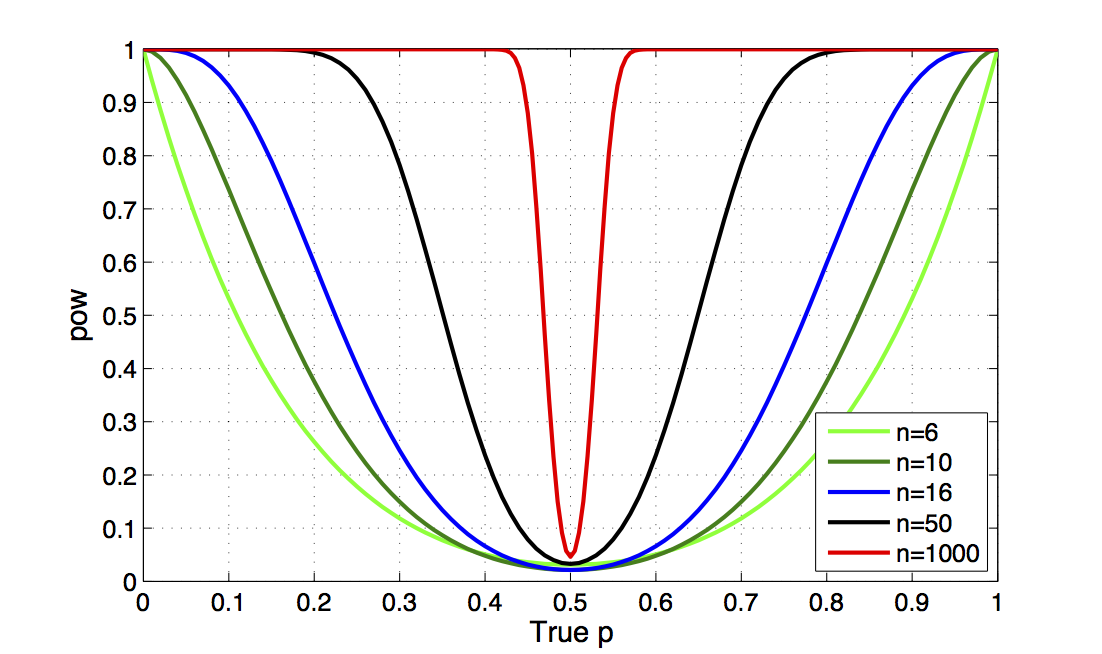
\includegraphics[width=0.8\textwidth]{powercurve.png}
		\end{center}
	}
\end{frame}

\begin{frame}{Размер выборки}
%%%%%%%%%%%%%%%%%%%%%%%%%%%%%%%%%%%%%%%%%%%%%%%%%%%%%%%%%%%%%%%%%%%%%%%
%
%%%%%%%%%%%%%%%%%%%%%%%%%%%%%%%%%%%%%%%%%%%%%%%%%%%%%%%%%%%%%%%%%%%%%%%
	Особенности прикладной задачи: $1$ порция мартини содержит $55$~мл джина и $15$~мл вермута~--- суммарно около $25$~мл спирта.
	Смертельная доза алкоголя при массе тела $80$~кг составляет от $320$ до $960$~мл спирта в~зависимости от толерантности (от $13$ до $38$ мартини).

	\bigskip

	Обеспечение требуемой мощности: размеры выборки подбирается так, чтобы при размере отклонения от нулевой гипотезы не меньше заданного (например, вероятность выбора взболтанного мартини не меньше $0.75$) мощность была не меньше заданной.
\end{frame}


\begin{frame}{}{}
    \centering
    \bfseries
    \huge
     Параметрические критерии\\ проверки гипотез

%%%%%%%%%%%%%%%%%%%%%%%%%%%%%%%%%%%%%%%%%%%%%%%%%%%%%%%%%%%%%%%%%%%%%%%
% Параметрическим критериям проверки гипотез. Эти критерии называются параметрическими потому, что в проверяемых ими гипотезах высказывается предположение о значении параметра распределений, из которых предположительно взята выборка.
%%%%%%%%%%%%%%%%%%%%%%%%%%%%%%%%%%%%%%%%%%%%%%%%%%%%%%%%%%%%%%%%%%%%%%%
\end{frame}

\section{Нормальное распределение}
%%%%%%%%%%%%%%%%%%%%%%%%%%%%%%%%%%%%%%%%%%%%%%%%%%%%%%%%%%%%%%%%%%%%%%%
% Благодаря центральной предельной теореме и удобству вывода критериев для нормально распределённых выборок методы, основанные на предположении о нормальности данных, наиболее широко распространены.
%%%%%%%%%%%%%%%%%%%%%%%%%%%%%%%%%%%%%%%%%%%%%%%%%%%%%%%%%%%%%%%%%%%%%%%

\subsection{Некоторые задачи для нормальных выборок}
\begin{frame}[label=onesample]{Гипотезы о параметрах нормальных выборок}

    \structure{Одна выборка:}

    \begin{tikzpicture}[level distance=35mm]
    \node {$X^n \sim N(\mu, \sigma^2)$} [grow=right]
    child {
        node {$H_0\colon \mu = \mu_0$}
        child {
            node{$\sigma$ известна   \hyperlink{ztest1}{\beamerbutton{1}}}
        }
        child{
            node{$\sigma$ неизвестна \hyperlink{ttest1}{\beamerbutton{3}}}
        }
    }
    child {
        node {
            $H_0\colon \sigma = \sigma_0$
            \hyperlink{chitest1}{\beamerbutton{2}}
        }
    };
    \end{tikzpicture}

    \bigskip
    \structure{Две выборки:}
    \begin{tikzpicture}[level distance=35mm]
    \node {\parbox{3cm}{
            $X_1^{n_1} \sim N(\mu_1, \sigma_1^2)$,
            $X_2^{n_2} \sim N(\mu_2, \sigma_2^2)$
    }} [grow=right]
    child {
        node {$H_0\colon \mu_1 = \mu_2$}
        child{
            node {$X_1,X_2$ независимые}
            child {
                node{$\sigma_1$, $\sigma_2$ известны
                    \hyperlink{ztest2u}{\beamerbutton{4}}
                }
            }
            child{
                node{$\sigma_1$, $\sigma_2$ неизвестна
                   \hyperlink{ttest2u}{\beamerbutton{5}}
                }
            }
        }
        child {
            node {$X_1,X_2$ зависимые \hyperlink{ttest2p}{\beamerbutton{6}}}
        }
    }
    child {
        node {
            $H_0\colon \sigma_1 = \sigma_0$
            \hyperlink{ftest}{\beamerbutton{7}}
        }
    };
\end{tikzpicture}
\end{frame}



\subsection{Одновыборочные задачи}

\begin{frame}[label=ztest1]{\hyperlink{onesample}{\beamerbutton{1}} Z-критерий Стьюдента: $\mu=\mu_0$, $\sigma$ известна }
    \begin{itemize}
        \item Выборка $X \sim N\left(\mu, \sigma^2\right)$
        \item $H_0\colon \mu=\mu_0$,
        \qquad
            $H_1\colon \mu \neq \mu_0$
        \quad
        $H_1\colon \mu < \mu_0$
        \quad
        $H_1\colon \mu  > \mu_0$
        \item \structure{статистика:}\qquad
        \alert{$\displaystyle
        Z\left(X^n\right) = \frac{\bar{X}-\mu_0}{\sigma / \sqrt{n}}  \sim N(0,1)
        $}
        \item \structure{достигаемый уровень значимости:}
        $$
        p\left(Z\right) = \begin{cases}
            1-F_{N(0,1)}(Z), & H_1 \colon \mu>\mu_0, \\
            F_{N(0,1)}(Z), & H_1 \colon \mu < \mu_0, \\
            2\left(1-F_{N(0,1)}(|Z|)\right), & H_1 \colon \mu\neq\mu_0. \\
        \end{cases}
        $$
    \end{itemize}
    \medskip
    \hrule
    \medskip
    \centering
    \begin{tabular}{cc}
        $ H_1 \colon \mu<\mu_0$ & $ H_1 \colon \mu>\mu_0$
        \tabularnewline
        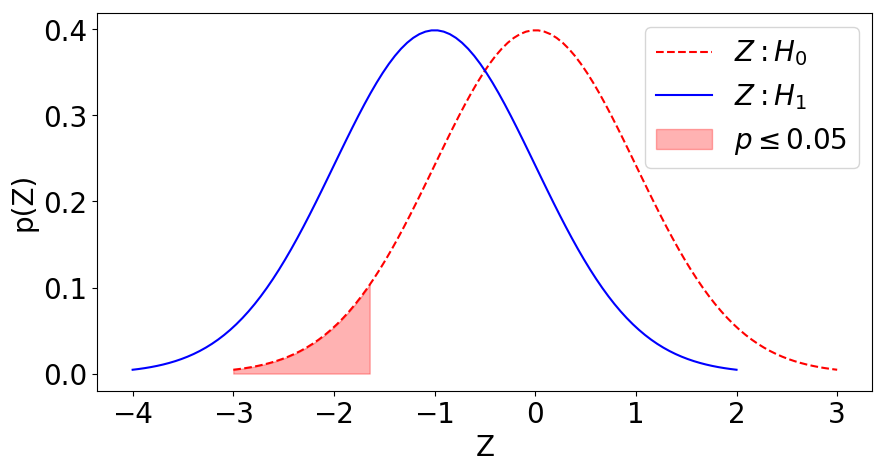
\includegraphics[width=0.35\textwidth]{z_less.png} &
        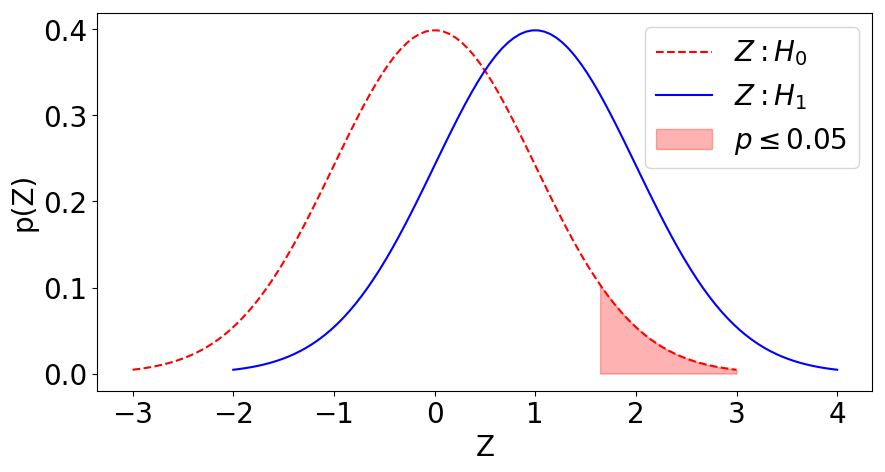
\includegraphics[width=0.35\textwidth]{z_more.png}
        \tabularnewline
    \end{tabular}
\end{frame}


\begin{frame}{\hyperlink{onesample}{\beamerbutton{1}} Пример  $\mu=\mu_0$, $\sigma$ известна }
    \begin{block}{Пример}
    Линия по производству пудры должна обеспечивать средний вес пудры в упаковке 4 грамма, заявленное стандартное отклонение~--- 1 грамм.

    В ходе инспекции выбрано 9 упаковок, средний вес продукта в них составляет 4.6 грамма.
    \end{block}
    \bigskip
    \begin{itemize}
    \item $H_0\colon$ средний вес пудры в упаковке соответствует норме.

    \item $H_1\colon$ средний вес пудры в упаковке не соответствует норме.

     $\Rightarrow p = 0.0719$, 95\% доверительный интервал для среднего веса~--- $\left[3.95, 5.25\right]$~г.

    $H_1\colon$ средний вес пудры в упаковке превышает норму  $\Rightarrow p = 0.0359,$ нижний 95\% доверительный предел для среднего веса~--- $4.05$~г.
    \end{itemize}
\textbf{Одностороннюю альтернативу можно использовать, если знак изменения среднего известен заранее.}

\end{frame}


\begin{frame}[label=ttest1]{\hyperlink{onesample}{\beamerbutton{3}} t-критерий Стьюдента: $\mu=\mu_0$, $\sigma$ неизвестна }
%%%%%%%%%%%%%%%%%%%%%%%%%%%%%%%%%%%%%%%%%%%%%%%%%%%%%%%%%%%%%%%%%%%%%
% Если дисперсия выборки неизвестна, вместо Z-критерия Стьюдента нужно применять t-критерий Стьюдента.
%Он основан на следующей идее: поскольку сигма неизвестна, то нужно в формуле статистики заменить сигма на S (выборочное стандартное отклонение).
%Такая статистика имеет уже не стандартное нормальное нулевое распределение, а распределение Стьюдента с числом степеней свободы n-1
% Чем больше объем выборки в задаче, тем меньше различий между t-критерием и Z-критерием.
%Это происходит по двум причинам: во-первых, чем больше n, тем точнее выборочная дисперсия $S^2$ оценивает теоретическую дисперсию.
%Во-вторых, с ростом n увеличивается число степеней свободы у нулевого распределения t-критерия, а чем больше степеней свободы у распределения Стьюдента, тем больше оно похоже на стандартное нормальное.
%Ранее уже упоминалось, что, начиная с 30 степеней свободы, распределение Стьюдента визуально неотличимо от стандартного нормального.
%Благодаря этим двум фактам для достаточно больших выборок знание истинного значения дисперсии не оказывает большого влияния на результат.
%%%%%%%%%%%%%%%%%%%%%%%%%%%%%%%%%%%%%%%%%%%%%%%%%%%%%%%%%%%%%%%%%%%%%

    \begin{itemize}
    \item Выборка $X \sim N\left(\mu, \sigma^2\right)$
    \item $H_0\colon \mu=\mu_0$,
    \qquad
    $H_1\colon \mu \neq \mu_0$
    \quad
    $H_1\colon \mu < \mu_0$
    \quad
    $H_1\colon \mu  > \mu_0$
    \item \structure{статистика:}\qquad
    \alert{$\displaystyle
        t\left(X^n\right) = \frac{\bar{X}-\mu_0}{s/\sqrt{n}}  \sim St(n-1)
        $}
    \item \structure{достигаемый уровень значимости:}
    $$
    p\left(t\right) = \begin{cases}
        1-F_{St(n-1)}(t), & H_1 \colon \mu>\mu_0, \\
        F_{st(n-1)}(t), & H_1 \colon \mu < \mu_0, \\
        2\left(1-F_{St(n-1)}(|t|)\right), & H_1 \colon \mu\neq\mu_0. \\
    \end{cases}
    $$
\end{itemize}
  \centering
  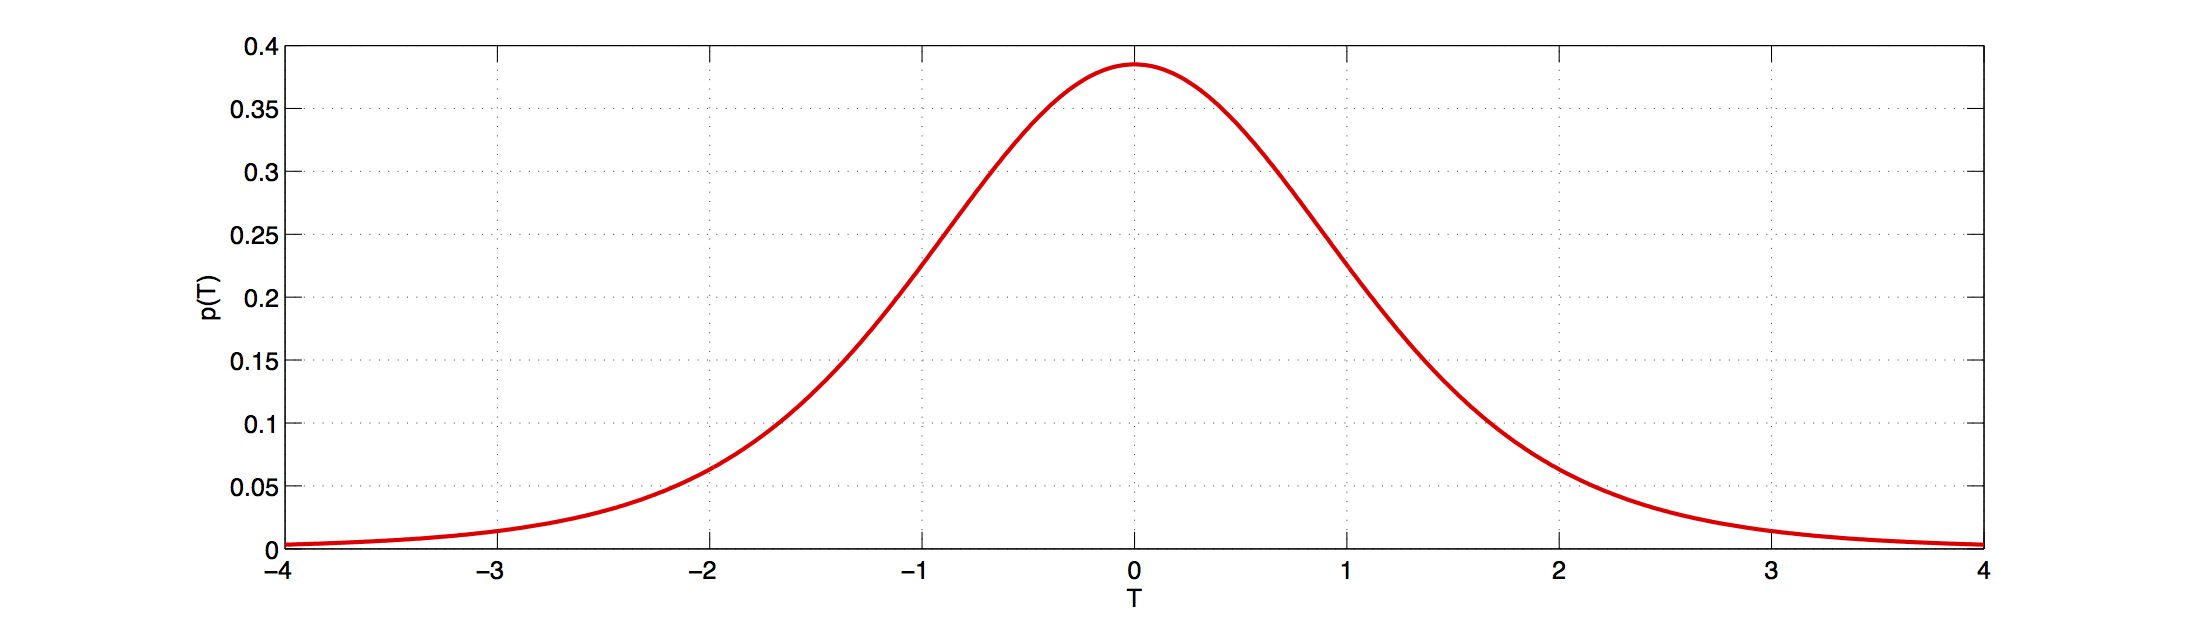
\includegraphics[width=0.7\textwidth]{stud.png}

    С ростом объёма выборки разница между t- и z-критериями уменьшается.
\end{frame}
\begin{frame}[allowframebreaks]{Пример:  $\mu=\mu_0$, $\sigma$ неизвестна}
%%%%%%%%%%%%%%%%%%%%%%%%%%%%%%%%%%%%%%%%%%%%%%%%%%%%%%%%%%%%%%%%%%%%%%%
%%  Вес при рождении — это очень важный показатель здоровья ребенка. Так, только 7\% детей рождаются с весом меньше 2.5 кг, однако на них приходится 70\% детских смертей.
%%%%%%%%%%%%%%%%%%%%%%%%%%%%%%%%%%%%%%%%%%%%%%%%%%%%%%%%%%%%%%%%%%%%%%%%
    \begin{block}{}
        Средний вес детей при рождении составляет 3300~г. В то же время, если мать ребёнка живёт за чертой бедности, то средний вес таких детей — 2800~г.

        С целью увеличить вес тех детей, чьи матери живут за чертой бедности, разработана программа ведения беременности.

        Чтобы проверить ее эффективность, проводится эксперимент. В нём принимают участие 25~женщин, живущих за чертой бедности. У всех них рождаются дети, и их средний вес составляет 3075~г, выборочное СКО~--- 500~г.

        Эффективна ли программа? Уровень значимости: $\alpha = 0.05$
     \end{block}
    \framebreak
    \begin{itemize}
        \item \structure{Вопрос 1:} Влияет ли программа не вес детей?
        \begin{itemize}
            \item $H_0\colon \mu=2800$~--- программа не влияет на вес детей.
            \item $H_1\colon \mu \neq 2800$ программа как-то влияет на вес детей.
            \item $t(X^n) = \frac{3075-2800}{500/\sqrt{25}} = 2.75$
            \item $F_{St(24)}(2.75) \approx 0.9944$\hfill \alert{\texttt{scipy.stats.t(24).cdf(t)}}
            \item $p(t) = 2\big(1-F_{St(24)}(2.75)\big)\approx 0.0111$
            \item $p(t)< \alpha=0.05$, поэтому влияние существенно.
            \item 95\% доверительный интервал для изменения веса~--- $\left[68.6, 481.4\right]$~г.
       \end{itemize}
       \medskip
        \item \structure{Вопрос 2:} увеличивается ли вес ребенка в следствие программы?
        \begin{itemize}
            \item $H_0\colon \mu=2800$~--- программа не влияет на вес детей.
            \item $H_1\colon \mu>2800 $ программа увеличивает вес детей
            \item $p(t) = 2\big(1-F_{St(24)}(2.75)\big)\approx 0.0111$
             $p(t) = 1- F_{St(24)}(2.75) \approx 0.0056$
             \item 95\% нижний доверительный предел для увеличения веса~--- $103.9$~г.
        \end{itemize}
    \end{itemize}
\end{frame}



\begin{frame}[label=chitest1]{\hyperlink{onesample}{\beamerbutton{2}} Критерий хи-квадрат: $\sigma=\sigma_0$}

\begin{itemize}
    \item Выборка$X^n=\left(X_1,\ldots,X_n\right), X\sim N\left(\mu, \sigma^2\right)$
    \item $H_0\colon \sigma=\sigma_0$,
    \qquad
    $H_1\colon \sigma \neq \sigma_0$
    \quad
    $H_1\colon \sigma < \sigma_0$
    \quad
    $H_1\colon \sigma  > \sigma_0$

    \item \structure{статистика:}\qquad
    \alert{$\displaystyle \chi^2\left(X^n\right) = \frac{(n-1)S^2}{\sigma_0^2}$}
    \item \structure{достигаемый уровень значимости:}
     $$p\left(\chi^2\right) = \begin{cases}
        1-F_{\chi^2_{n-1}}(\chi^2), 																  & H_1 \colon \sigma>\sigma_0, \\
        F_{\chi^2_{n-1}}(\chi^2),    																   & H_1 \colon \sigma<\sigma_0, \\
        2 \min\left( 1-F_{\chi^2_{n-1}}(\chi^2), F_{\chi^2_{n-1}}(\chi^2) \right),  & H_1 \colon \sigma\neq\sigma_0. \\
    \end{cases}$$
  \end{itemize}
  \centering
    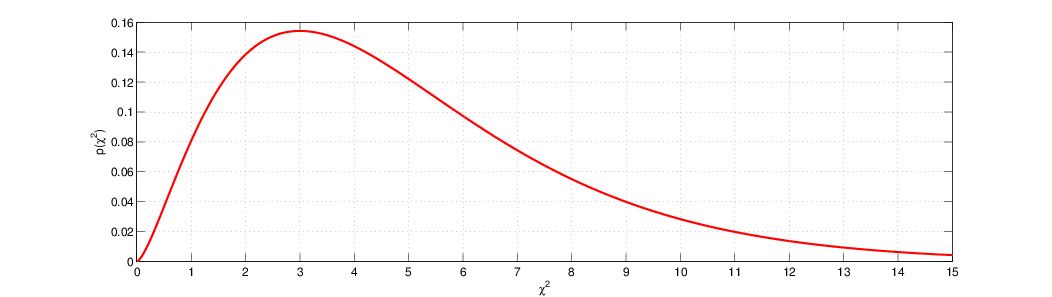
\includegraphics[width=0.7\textwidth]{chi2.png}

\end{frame}
\begin{frame}[allowframebreaks]{Пример:  $\sigma=\sigma_0$ }
        \begin{block}{}
            При производстве микрогидравлической системы делается инъекция жидкости.
            Дисперсия объёма жидкости~--- критически важный параметр, установленный стандартом на уровне 9~кв.\,мл.
            В выборке из 25~микрогидравлических систем выборочная дисперсия объёма жидкости составляет 12~кв.\,мл.
        \end{block}
        \begin{itemize}
            \item \structure{Вопрос 1:} Существенно ли отклонение дисперсиипри уровне значимости $\alpha=0.05$?
            \begin{itemize}
                \item $H_0\colon \sigma = 9$ дисперсия объёма жидкости соответствует стандарту.
                \item  $H_1\colon \sigma \neq 9$ дисперсия объёма жидкости не соответствует стандарту
                \item $\chi^2(X^n)= \frac{(25-1)\cdot 12}{9} = 32$
                \item $F_{\chi^2_{25-1}}(32) \approx 0.8730$\hfill
                \alert{\texttt{scipy.stats.chi2(24).cdf(32)}}
                \item $p(\chi^2) = 2\min\{(1-F_{\chi^2_{24}}(32), F_{\chi^2_{24}}(32))\} \approx 0.254$
                \item $p(\chi^2) > 0.05$ нет причин считать дисперсию не соответствующей стандарту
                \item 95\% доверительный интервал для дисперсии~--- $\left[7.3, 23.2\right]$~кв.\,мл.
           \end{itemize}
           \framebreak
            \item \structure{Вопрос 2:} Действительно ли дисперсия объёма жидкости превышает допустимое значениё
            \begin{itemize}
                \item  $H_1\colon \sigma > 9$ дисперсия объёма жидкости превышает допустимое значение
                \item $p(\chi^2) = 1-F_{\chi^2_{25-1}}(32) \approx  0.127 $
                \item $p(\chi^2) > 0.05$ нет причин считать дисперсию не соответствующей стандарту
                \item  односторонний нижний 95\% доверительный предел~--- $7.9$~кв.\,мл.
           \end{itemize}
       \end{itemize}
\end{frame}

\begin{frame}{Выбор альтернативной гипотезы}
%%%%%%%%%%%%%%%%%%%%%%%%%%%%%%%%%%%%%%%%%%%%%%%%%%%%%%%%%%%%%%%%%%%%%%%
% Рассмотренный пример показывает, что, используя одностороннюю альтернативу вместо двусторонней, можно получить достигаемый уровень значимости в два раза меньше.
%В данной задаче это было не критично, поскольку оба достигаемых уровня значимости маленькие.
%Но иногда может оказаться, что p-value при двусторонней альтернативе больше магического порога в 0.05, а при односторонней альтернативе — меньше.
%То есть, используя одностороннюю альтернативу вместо двухсторонней, можно отвергнуть нулевую гипотезу.
%В таком случае кажется, что можно всегда использовать одностороннюю альтернативу, однако это нечестно.
%Альтернатива может быть односторонней только в некоторых случаях.
% Во-первых, если среднее должно изменится в какую-то определенную сторону и изменение в противоположную сторону невероятно.
% Во-вторых, направление изменения нужно определить до получения данных.
% Если односторонняя альтернатива выбирается после того, как данные получены, и она выбирается так, что ее знак соответствует знаку изменения выборочного среднего относительно mu0, то это — переобучение, и так делать нельзя.
%%%%%%%%%%%%%%%%%%%%%%%%%%%%%%%%%%%%%%%%%%%%%%%%%%%%%%%%%%%%%%%%%%%%%%%
\centering
\large
По умолчанию используется двухсторонняя гипотеза

\bigskip

Одностороннюю альтернативу можно использовать, если знак изменения среднего известен заранее.

\bigskip

\alert{Альтернатива должна выбираться до получения данных!}
\end{frame}


\subsection{Двухвыборочные задачи}
\begin{frame}[label=ztest2u]{\hyperlink{onesample}{\beamerbutton{4}} Сравнение средних выборок. Z-критерий Стьюдента}{выборки не связаны, $\sigma_1, \sigma_2$ известны}
    \begin{itemize}
            \item \structure{Выборки:}

             $X_1^{n_1}=\left(X_{11},\ldots,X_{1n_1}\right), X_{1} \sim N\left(\mu_1, \sigma_1^2\right)$

            $X_2^{n_2}=\left(X_{21},\ldots,X_{2n_2}\right), X_{2} \sim N\left(\mu_2, \sigma_2^2\right)$
            \item $\sigma_1, \sigma_2$ известны \\
            \item  $H_0\colon \mu_1=\mu_2$,\qquad
             $H_1\colon \mu_1 \neq \mu_2$,
             $H_1\colon \mu_1 < \mu_2$,
             $H_1\colon \mu_1  >\mu_2$.
            \item Статистика: \alert{$\displaystyle Z\left(X_1^{n_1}, X_2^{n_2}\right) = \frac{\bar{X}_1-\bar{X}_2}{\sqrt{\frac{\sigma_1^2}{n_1}+\frac{\sigma_2^2}{n_2}}} \sim N(0,1)$}
            \item \structure{достигаемый уровень значимости:}
            $$
            p\left(Z\right) = \begin{cases}
                1-F_{N(0,1)}(Z), & H_1 \colon \mu_1>\mu_2, \\
                F_{N(0,1)}(Z), & H_1 \colon \mu_1 < \mu_2, \\
                2\left(1-F_{N(0,1)}(|Z|)\right), & H_1 \colon \mu_1\neq\mu_2. \\
            \end{cases}
            $$
%          \item В Python:
    \end{itemize}
%    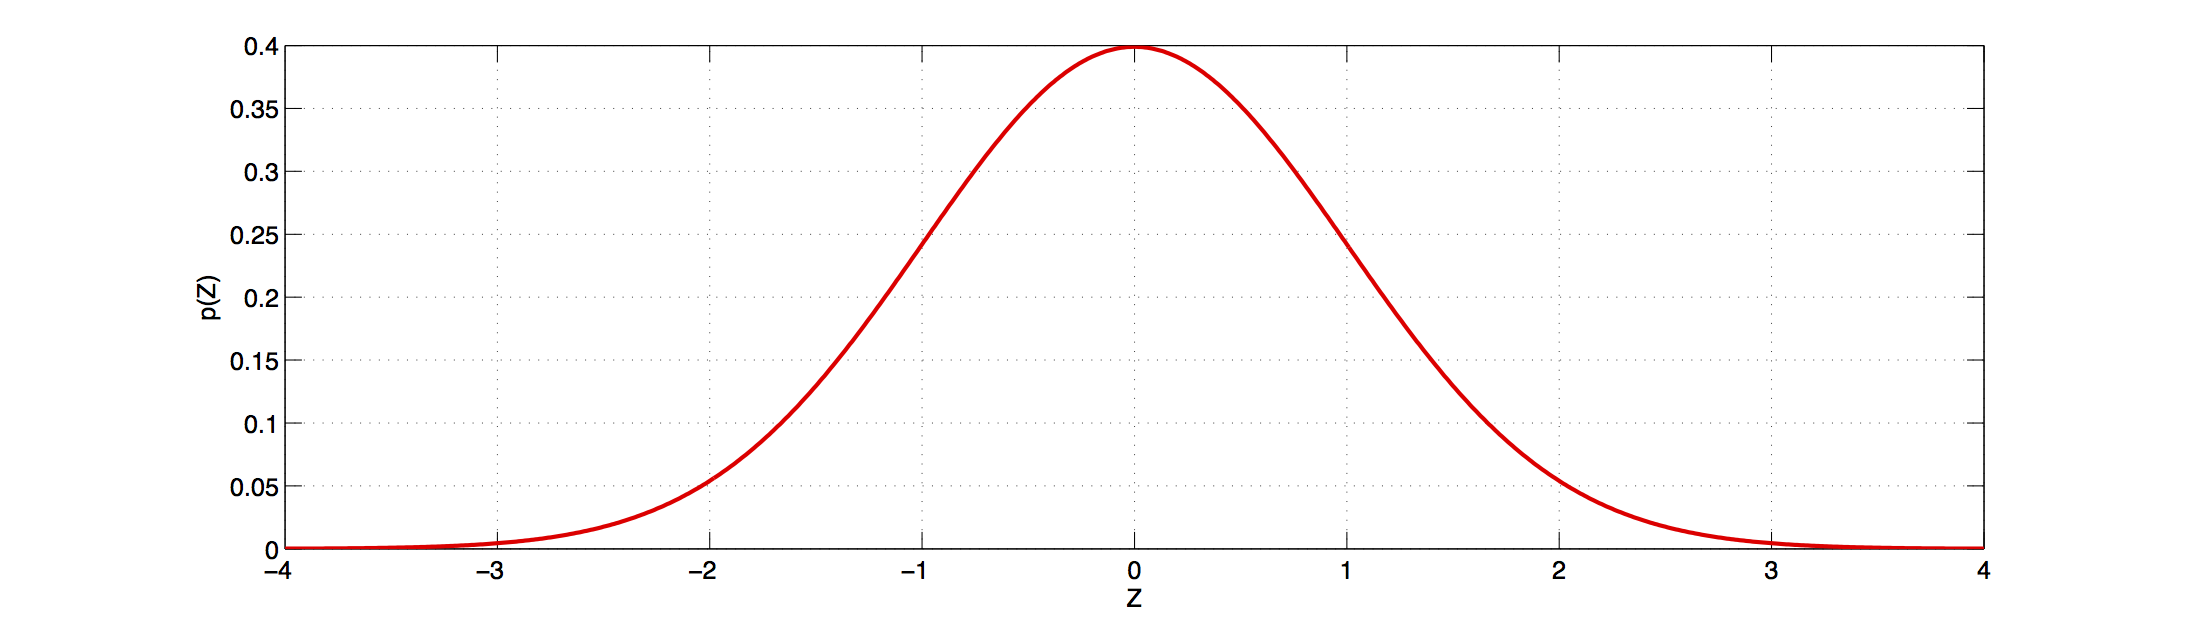
\includegraphics[width=0.7\textwidth]{norm.png}
\end{frame}
%\begin{frame}{Пример: Сравнение средних выборок. $\sigma_1, \sigma_2$ известны }
%
%\begin{block}{Пример, Kanji, критерий 3}
%известно, что одна из линий по расфасовке чипсов даёт упаковки с более вариабельным весом продукта, чем вторая. Дисперсии равны 0.000576~$\text{г}^2$ и 0.001089~$\text{г}^2$ соответственно, средние значения веса в~выборках из~13 и~8~элементов~--- 80.02~г и 79.98~г.
%    \end{block}
%    \bigskip
%
%    $H_0\colon$ средний вес продукта в упаковках, произведённых на двух линиях, совпадает.
%
%    $H_1\colon$ средние веса продукта в упаковках, произведённых на двух линиях, различаются $\Rightarrow p = 0.001,$ 95\%~доверительный интервал для разности~--- $\left[0.039, 0.041\right]$.
%\end{frame}



\begin{frame}[label=ttest2u]{\hyperlink{onesample}{\beamerbutton{4}} Сравнение средних выборок. t-критерий Стьюдента}{выборки не связаны, $\sigma_1, \sigma_2$ неизвестны}

%%%%%%%%%%%%%%%%%%%%%%%%%%%%%%%%%%%%%%%%%%%%%%%%%%%%%%%%%%%%%%%%%%%%%%%
% В более сложном случае дисперсии выборок неизвестны. Можно действовать по аналогии с одновыборочным случаем: в формуле для Z-критерия заменить все неизвестные сигмы на их выборочные оценки S1 и S2. Получится t-статистика.
% У этой задачи есть две проблемы. Во-первых, число степеней свободы ? у этого нулевого распределения Стьюдента вычисляется по достаточно сложной формуле. Во-вторых, нулевое распределение t-статистики не точное, а приближенное. Точного решения (то есть точного нулевого распределения для такой статистики) не существует. Эта проблема называется проблемой Беренца-Фишера: невозможно точно сравнить средние значение в двух выборках, дисперсии которых неизвестны.
% Однако рассмотренная аппроксимация достаточно точна в двух ситуациях. Во-первых, если выборки X1 и X2 одинакового объема, то есть n1 = n2. Во-вторых, если знак неравенства между n1 и n2 такой же, как между сигма1 и сигма2, то есть выборка с большей дисперсией по размеру не может быть меньше другой выборки. Если это условие выполнено, то можно использовать t-критерий Стьюдента и не переживать о точности аппроксимации. Если это не так, то возникает проблема: критерий Стьюдента перестает правильно работать, и вероятность ошибок первого рода начинает превышать уровень значимости ?. Это проблема не только критерия Стьюдента, она возникает при проверке любым способом гипотезы о равенстве средних в двух выборках с разной дисперсией. Поэтому, сравнивая средние значения в двух выборках, важно всегда следить за тем, чтобы выборка с большей дисперсией всегда была не меньшего объема, чем вторая выборка.
%%%%%%%%%%%%%%%%%%%%%%%%%%%%%%%%%%%%%%%%%%%%%%%%%%%%%%%%%%%%%%%%%%%%%%%

    \begin{itemize}
        \item \structure{Выборки:}

        $X_1^{n_1}=\left(X_{11},\ldots,X_{1n_1}\right), X_{1} \sim N\left(\mu_1, \sigma_1^2\right)$

        $X_2^{n_2}=\left(X_{21},\ldots,X_{2n_2}\right), X_{2} \sim N\left(\mu_2, \sigma_2^2\right)$
        \item $\sigma_1, \sigma_2$ неизвестны
        \item  $H_0\colon \mu_1=\mu_2$,\qquad
        $H_1\colon \mu_1 \neq \mu_2$,
        $H_1\colon \mu_1 < \mu_2$,
        $H_1\colon \mu_1  >\mu_2$.
        \item Статистика: \alert{$\displaystyle
        T\left(X_1^{n_1}, X_2^{n_2}\right) = \frac{\bar{X}_1-\bar{X}_2}{\sqrt{\frac{S_1^2}{n_1} + \frac{S_2^2}{n_2}}} \approx St(\nu)$}, \qquad $\nu = \frac{\left( \frac{S_1^2}{n_1} + \frac{S_2^2}{n_2} \right)^2}{ \frac{S_1^4}{n_1^2(n_1-1)} + \frac{S_2^4}{n_2^2(n_2-1)} }$

        \item \structure{достигаемый уровень значимости:}
        $$
        p\left(t\right) = \begin{cases}
            1-F_{St(n-1)}(t), & H_1 \colon \mu>\mu_0, \\
            F_{st(n-1)}(t), & H_1 \colon \mu < \mu_0, \\
            2\left(1-F_{St(n-1)}(|t|)\right), & H_1 \colon \mu\neq\mu_0. \\
        \end{cases}
        $$

        %          \item В Python:
    \end{itemize}
    %    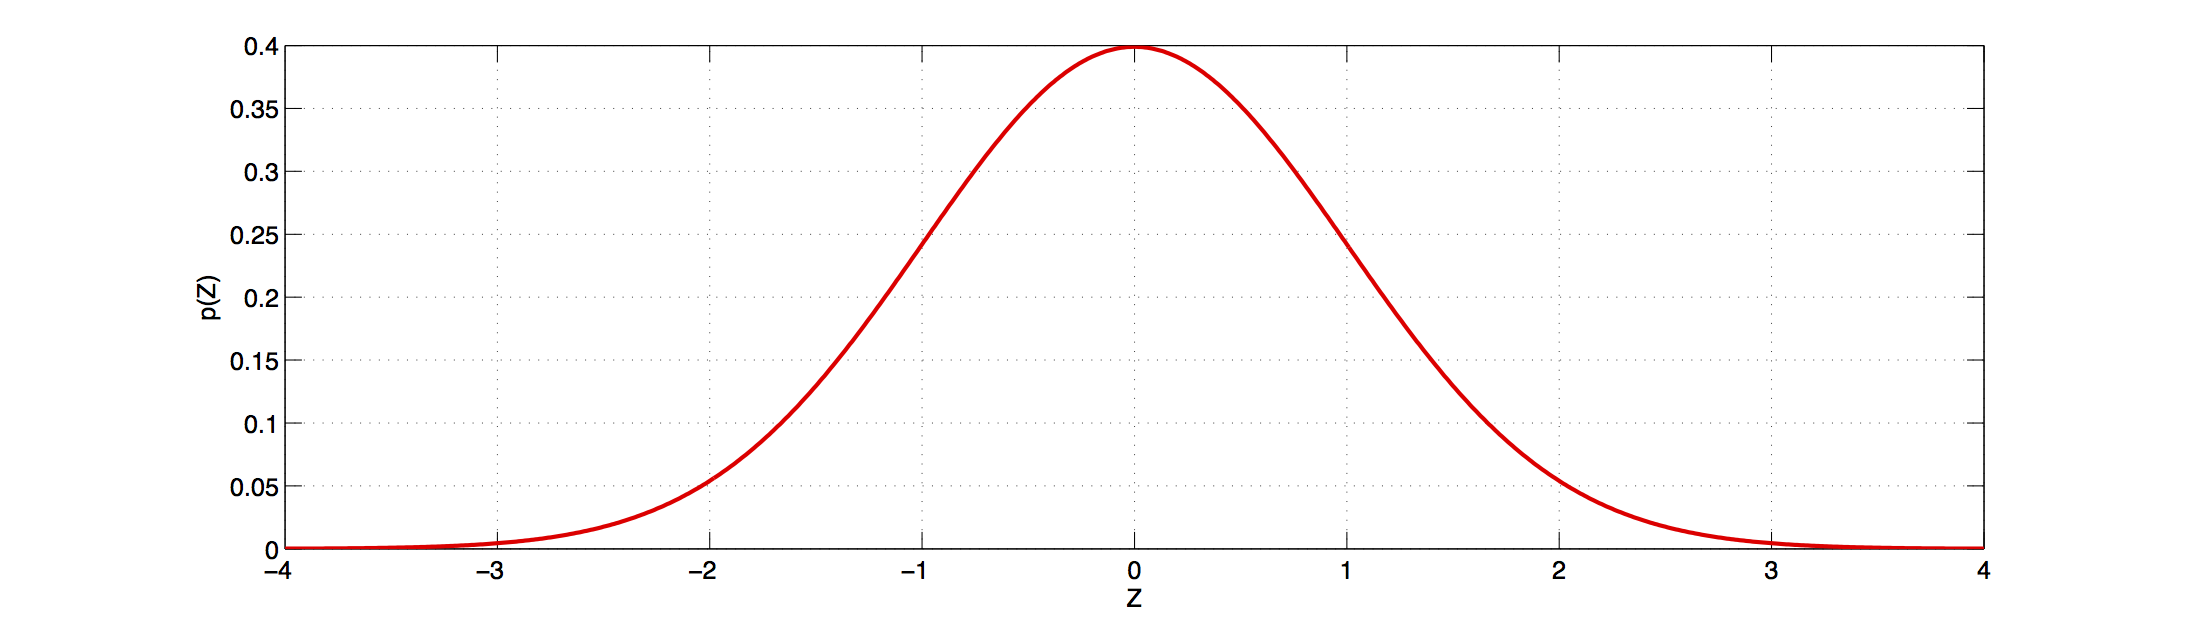
\includegraphics[width=0.7\textwidth]{norm.png}

    \textbf{Приближение достаточно точно при} $n_1=n_2$ \textbf{или} $\left[n_1>n_2\right] = \left[\sigma_1>\sigma_2\right].$
\end{frame}
%
%\begin{frame}[label=ttest2u]{\hyperlink{twosample}{\beamerbutton{5}} t-критерий Стьюдента / Аспина-Уэлша (проблема Беренца-Фишера)}
%\only<1>{
%
%    \begin{center}
%        \begin{tabular}{rl}
%            выборки:                        & $X_1^{n_1}=\left(X_{11},\ldots,X_{1n_1}\right), X_{1}\sim N\left(\mu_1, \sigma_1^2\right)$ \\
%            & $X_2^{n_2}=\left(X_{21},\ldots,X_{2n_2}\right), X_{2}\sim N\left(\mu_2, \sigma_2^2\right)$ \\
%            & $\sigma_1, \sigma_2$ неизвестны \\
%            нулевая гипотеза:               & $H_0\colon \mu_1=\mu_2$ \\
%            альтернатива:                   & $H_1\colon \mu_1<\neq>\mu_2$ \\
%            статистика:                     & $T\left(X_1^{n_1}, X_2^{n_2}\right) = \frac{\bar{X}_1-\bar{X}_2}{\sqrt{\frac{S_1^2}{n_1} + \frac{S_2^2}{n_2}}}$\\
%            & $\nu = \frac{\left( \frac{S_1^2}{n_1} + \frac{S_2^2}{n_2} \right)^2}{ \frac{S_1^4}{n_1^2(n_1-1)} + \frac{S_2^4}{n_2^2(n_2-1)} }$ \\
%            нулевое распределение:          & $\approx St(\nu)$\\
%        \end{tabular}
%        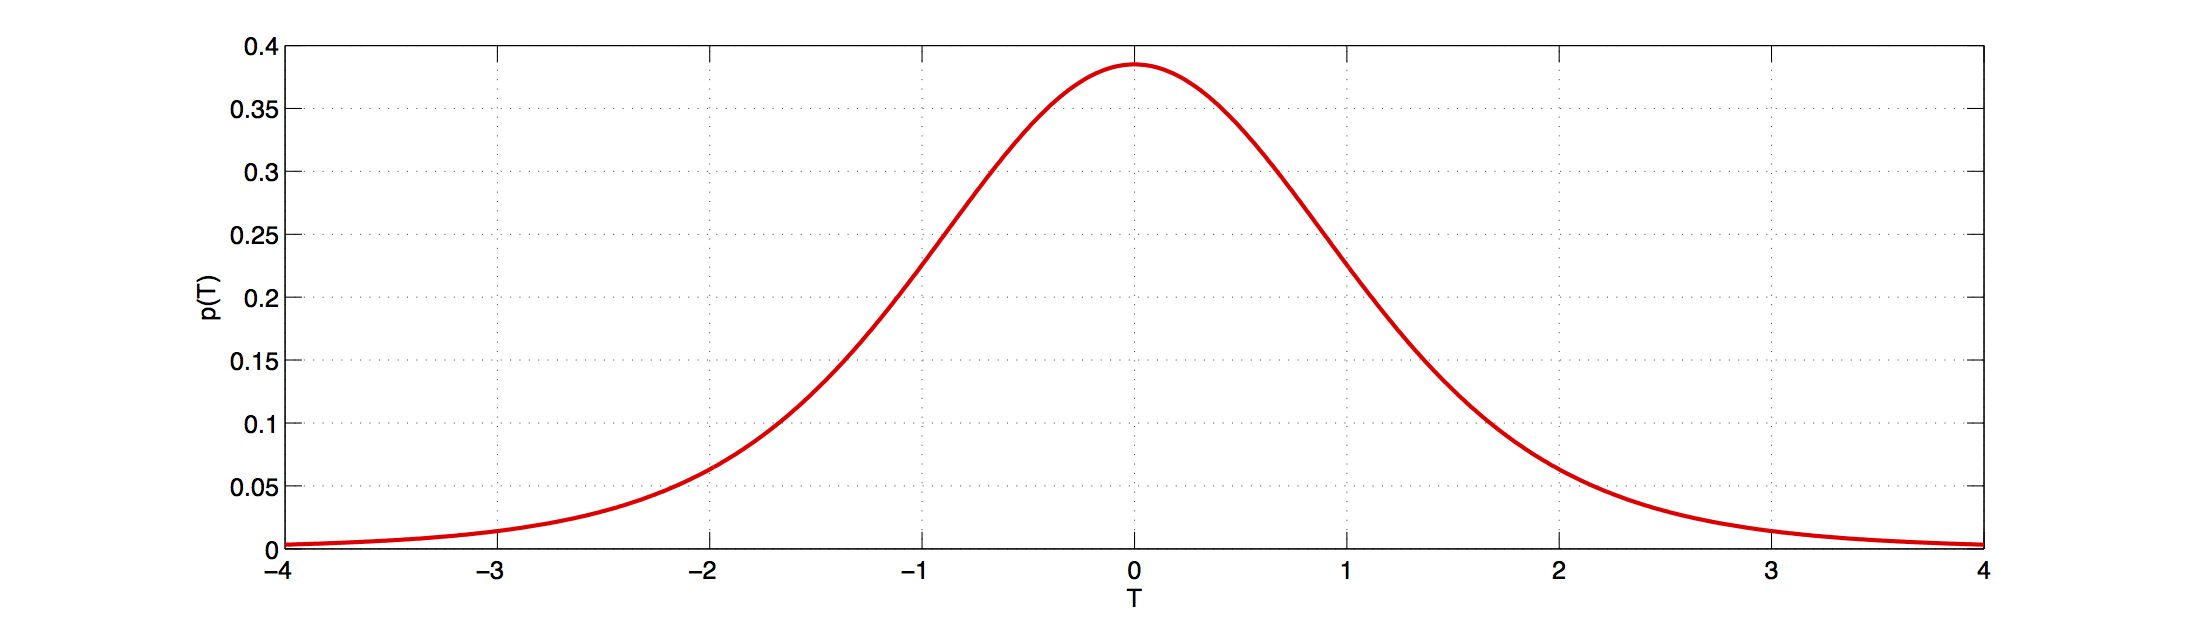
\includegraphics[width=0.7\textwidth]{stud.png}
%    \end{center}
%
%}
%
%\only<2>{
%%%%%%%%%%%%%%%%%%%%%%%%%%%%%%%%%%%%%%%%%%%%%%%%%%%%%%%%%%%%%%%%%%%%%%%%
%% General Social Survey. Это социологический опрос, который проводится на достаточно больших выборках в США уже больше 40 лет. В этом опросе очень много вопросов, которые задают респондентам, здесь будет рассматриваться только один.
%%%%%%%%%%%%%%%%%%%%%%%%%%%%%%%%%%%%%%%%%%%%%%%%%%%%%%%%%%%%%%%%%%%%%%%%
%\small
%\begin{block}{Пример}
% В 1974 году 108 респондентов GSS работали неполный день, в 2014~--- 196. Для каждого из них известно количество рабочих часов за неделю, предшествующую опросу.
%
%\begin{figure}
%    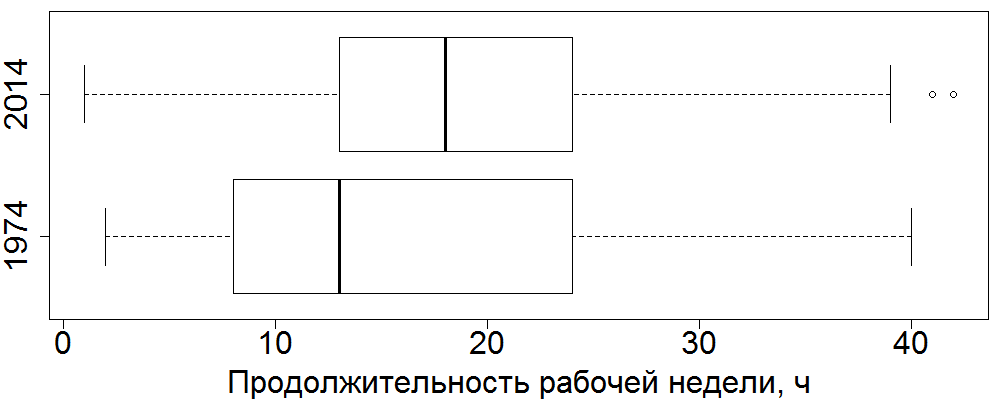
\includegraphics[width=0.75\textwidth]{hpw.png}
%\end{figure}
%Изменилось ли среднее время работы у работающих неполный день?
%\end{block}
%\bigskip
%
%$H_0\colon$ среднее время работы не изменилось, $\mu_1=\mu_2$.
%
%$H_0\colon$ среднее время работы изменилось, $\mu_1\neq\mu_2$.
%
%\bigskip
%
%t-критерий: $p=0.02707$, средняя продолжительность рабочей недели увеличилась на $2.57$~часов ($95$\% доверительный интервал~--- $\left[0.29, 4.85\right]$~ч).
%}
%\end{frame}

\begin{frame}[label=ttest2p]{\hyperlink{onesample}{\beamerbutton{6}} Сравнение средних связанных выборок. t-критерий Стьюдента}{выборки связаны}
%%%%%%%%%%%%%%%%%%%%%%%%%%%%%%%%%%%%%%%%%%%%%%%%%%%%%%%%%%%%%%%%%%%%%%%
% В числителе T-статистики стоит разность средних Х1 и X2. Это то же самое, что среднее X1 ? X2. Таким образом, t- критерий для двух связанных выборок эквивалентен одновыборочному t-критерию, примененному к выборке попарных разностей.
%%%%%%%%%%%%%%%%%%%%%%%%%%%%%%%%%%%%%%%%%%%%%%%%%%%%%%%%%%%%%%%%%%%%%%%
    \begin{itemize}
        \item \structure{Выборки:}

            $X_1^{n_1}=\left(X_{11},\ldots,X_{1n_1}\right), X_{1} \sim N\left(\mu_1, \sigma_1^2\right)$

            $X_2^{n_2}=\left(X_{21},\ldots,X_{2n_2}\right), X_{2} \sim N\left(\mu_2, \sigma_2^2\right)$
        \item выборки связаны
        \item  $H_0\colon \mu_1=\mu_2$,\qquad
            $H_1\colon \mu_1 \neq \mu_2$,
            $H_1\colon \mu_1 < \mu_2$,
            $H_1\colon \mu_1  >\mu_2$.
        \item Статистика: \alert{$\displaystyle
            t\left(X_1^{n_1}, X_2^{n_2}\right) = \frac{\bar{X}_1-\bar{X}_2}{S/\sqrt{n}} \sim  St(n-1)$}, \quad
            $S = \sqrt{ \frac1{n-1} \sum\limits_{i=1}^n \left(D_i-\bar{D}\right)^2 }$,
            \quad $D_i = X_{1i}-X_{2i},
            \quad \bar{D} = \frac{1}{n}\sum_i D_i$
        \item \structure{достигаемый уровень значимости:}
            $$
                p\left(t\right) = \begin{cases}
                    1-F_{St(n-1)}(t), & H_1 \colon \mu>\mu_0, \\
                    F_{st(n-1)}(t), & H_1 \colon \mu < \mu_0, \\
                    2\left(1-F_{St(n-1)}(|t|)\right), & H_1 \colon \mu\neq\mu_0. \\
                \end{cases}
            $$

    %          \item В Python:
    \end{itemize}
\end{frame}
\begin{frame}{Пример: сравнение средних связанных выборок}
    \begin{block}{Пример, Kanji, критерий 10}
    На 10 испытуемых сравниваются два лекарства против респираторного заболевания.
    Каждый из испытуемых вдыхает первое лекарство с помощью ингалятора, после чего проходит упражнение беговой дорожке.
    Измеряется время достижения максимальной нагрузки.
    Затем после периода восстановления эксперимент повторяется со вторым лекарством.
    \end{block}
    \bigskip
    \begin{itemize}
    \item $H_0\colon$ время достижения максимальной нагрузки не отличается для исследуемых лекарств.

    \item $H_1\colon$ время достижения максимальной нагрузки  для исследуемых лекарств отличается

     \item $p=0.916;$

     \item 95\% доверительный интервал для разности средних $\left[-2.1, 0.9\right].$
    \end{itemize}
\end{frame}

\begin{frame}{Пример}
    \only<1>{
        \begin{block}{}
        Пусть имеются следующие связные выборки:
        \begin{align*}
        X_1^n, & \;\; X_1\sim N(0,1), \\
        X_2^n, & \;\; X_2 = X_1 + \varepsilon, \;\; \varepsilon \sim N(0.1, 0.25) \Rightarrow X_2 \sim N(0.1, 1.25);
        \end{align*}
        требуется оценить разность $\Delta=\mathbb{E}X_1-\mathbb{E}X_2.$
        \end{block}

        1. Если \textbf{попарные соответствия элементов известны}, лучшая оценка $\hat{\Delta}_p = \frac1{n}\sum\limits_{i=1}^n\left(X_{1i}-X_{2i}\right)$ имеет дисперсию
        $$\mathbb{D}\hat{\Delta}_p = \frac1{n^2}\sum_{i=1}^n \mathbb{D}\left(X_{1i} - X_{2i}\right) = \frac1{n} \mathbb{D}\varepsilon = \frac1{2n};$$
        мощность 0.8 достигается при $n\approx200$.

        2. Если же \textbf{попарные соответствия неизвестны}, лучшая оценка~---  $\hat{\Delta}_i = \bar{X}_1 - \bar{X}_2$; её дисперсия:

        $$\mathbb{D}\hat{\Delta}_i = \frac1{n^2}\sum_{i=1}^n \mathbb{D}X_{1i} + \frac1{n^2}\sum_{i=1}^n \mathbb{D}X_{2i} = \frac1{n} + \frac{5}{4n} = \frac{9}{4n}$$
        --- в 4.5 раза больше; мощность 0.8 достигается при $n\approx1900$.
    }
\end{frame}

\begin{frame}[label=ftest]{\hyperlink{onesample}{\beamerbutton{7}} F-критерий Фишера. Гипотеза о дисперсиях}
    \begin{itemize}
        \item Выборки:

            $X_1^{n_1}=\left(X_{11},\ldots,X_{1n_1}\right), X_{1} \sim N\left(\mu_1, \sigma_1^2\right)$

            $X_2^{n_2}=\left(X_{21},\ldots,X_{2n_2}\right), X_{2} \sim N\left(\mu_2, \sigma_2^2\right)$

        \item $H_0\colon \sigma_1=\sigma_2$,\qquad
            $H_1\colon \sigma_1 \neq \sigma_2$,
            $H_1\colon \sigma_1 < \sigma_2$,
            $H_1\colon \sigma_1 > \sigma_2$.
        \item Статистика:
            \alert{$
                F\left(X_1^{n_1}, X_2^{n_2}\right) = \frac{S_1^2}{S_2^2} \sim F(n_1-1, n_2-1)
            $}
        \item \structure{достигаемый уровень значимости:}
            $$
                p\left(F\right) = \begin{cases}
                    \mathcal{F}_{F_{n_1-1,n_2-1}}(1/F), &
                                H_1 \colon \sigma_1>\sigma_2, \\
                    \mathcal{F}_{F_{n_1-1,n_2-1}}(F), &  H_1 \colon \sigma_1 < \sigma_2, \\
                    2\min\left\{\mathcal{F}_{F_{n_1-1,n_2-1}}(F), \mathcal{F}_{F_{n_1-1,n_2-1}}(1/F)\right\}, & H_1 \colon \sigma_1 \neq \sigma_2 \\
                \end{cases}
            $$
        % \item В Python:
    \end{itemize}
    Критерий Фишера неустойчив к отклонениям от нормальности даже асимптотически.
\end{frame}


\begin{frame}{\hyperlink{onesample}{\beamerbutton{7}} F-критерий Фишера. Гипотеза о дисперсиях}{Требования к выборкам}
    \begin{enumerate}
        \item \structure{Нормальность распределения:} Каждая из групп, между которыми проводится сравнение, должна иметь нормальное распределение данных. Это условие особенно важно, когда размеры выборок малы (Тест Шапиро).
        \item \structure{Гомогенность дисперсий:} Дисперсии внутри каждой из групп должны быть приблизительно равны.  (тест Левена или тест Бартлетта).

        \item \structure{Независимость выборок:} Выборки в каждой из групп должны быть независимыми друг от друга.

    \end{enumerate}

\end{frame}

%\begin{frame}{Пример: гипотеза о дисперсиях}
%   \begin{block}{ NIST/industry ceramics consortium for strength optimization of ceramic, 1996}
%    Собраны данные о прочности материала 440~керамических изделий из двух партий по 220 в каждой.
%
%    Одинакова ли дисперсия прочности в разных партиях?
%    \end{block}
%    \begin{center}
%            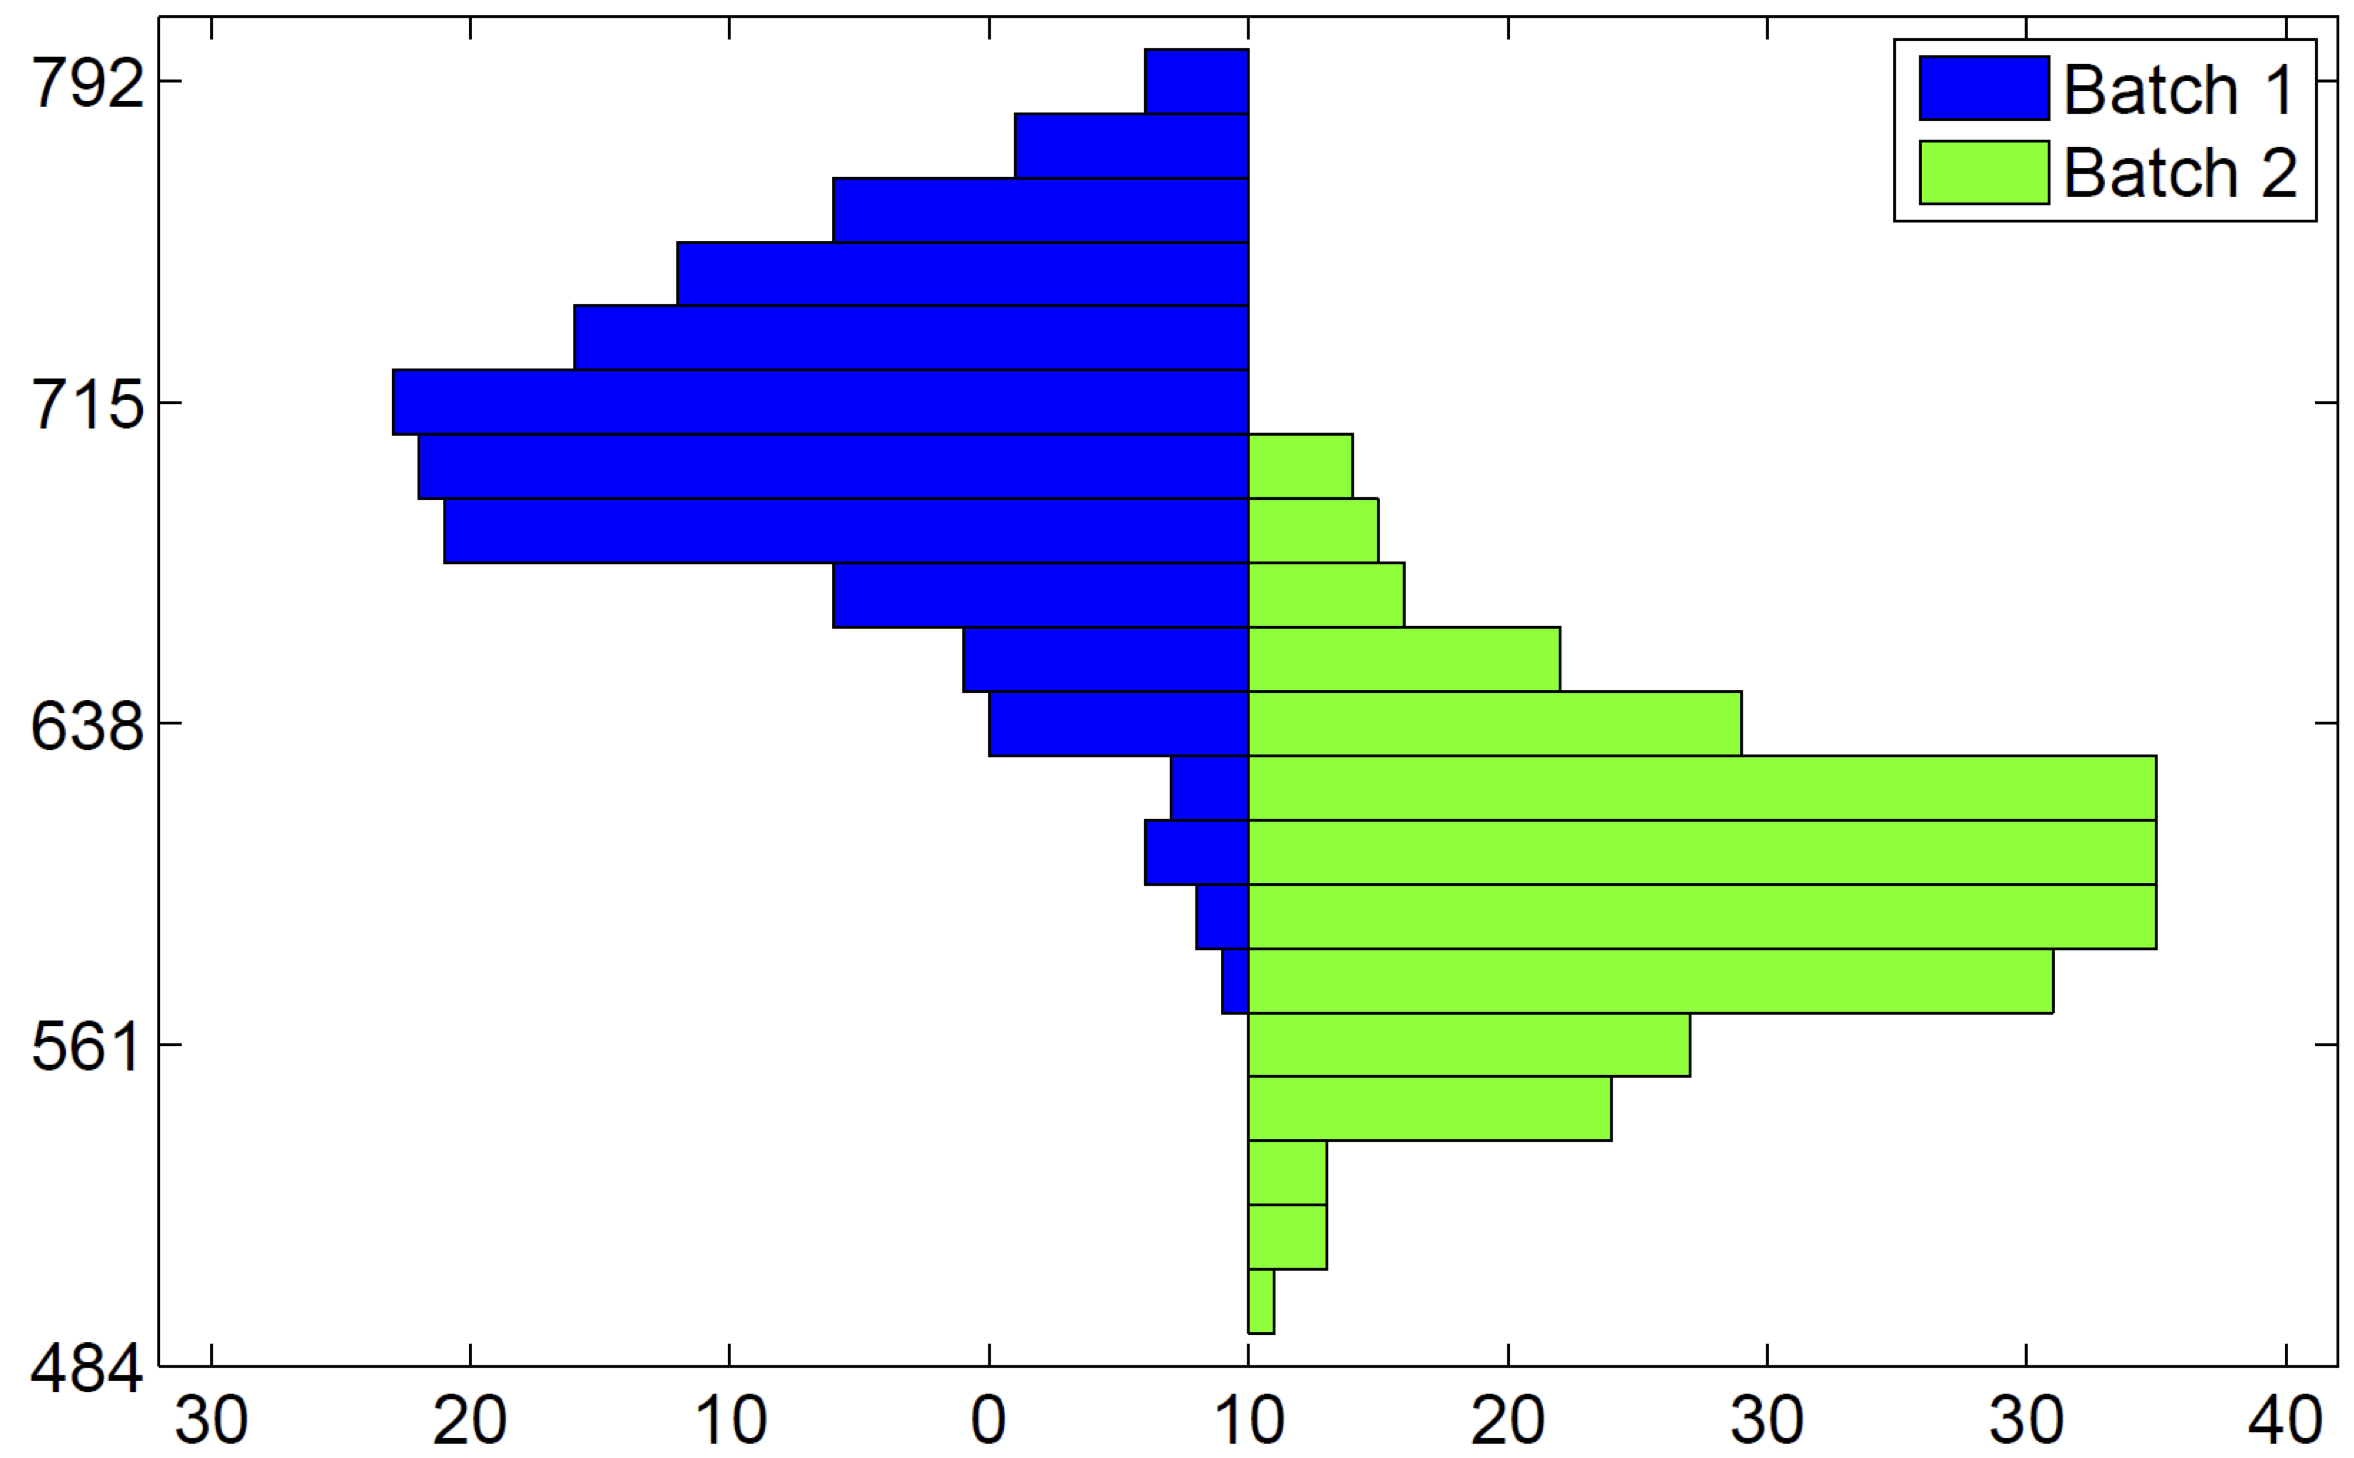
\includegraphics[width=0.3\textwidth]{ceramics.png}
%    \end{center}
%%			\
%%			Гипотезы нормальности не отклоняются критерием Шапиро-Уилка ($p_1=0.2062, p_2=0.7028$).
%    \begin{itemize}
%        \item
%        \item Критерий Фишера: $p=0.1721$,
%        \item   95\%-Доверительный интервал $\left[C_L, C_U\right]=\left[0.9225, 1.5690\right]$.
%    \end{itemize}
%\end{frame}

\subsection{Проверка нормальности}
\begin{frame}{}{}
    \centering
    \huge
    \bfseries
    Параметрические критерии проверки гипотез о законах распределения
\end{frame}

\begin{frame}{Критерий Харке"--~Бера}
    \begin{itemize}
        \item Выборка: $X^n=\left(X_1,\ldots,X_n\right)$
        \item $H_0\colon X \sim N\left(\mu,\sigma^2\right)$,\qquad $H_1\colon \lnot H_0$
        \item Cтатистика: \alert{$\chi^2\left(X^n\right) = \frac{n}{6}\left(\gamma_1^2 + \frac1{4} \gamma_2^2\right) \sim \chi^2_2$}

        $\gamma_1 = \mathbb{E} \left( \frac{X-\mathbb{E}X} {\sqrt{\mathbb{D}X}} \right)^3$,
        \qquad
        $\gamma_2 =  \frac{\mathbb{E}\left(X-\mathbb{E}X\right)^4}{\left(\mathbb{D}X\right)^2} - 3$
        \item достигаемый уровень значимости:
           $$
            p\left(\chi^2\right) = 1 - F_{\chi^2_2}\left(\chi^2\right)
           $$
    \end{itemize}
    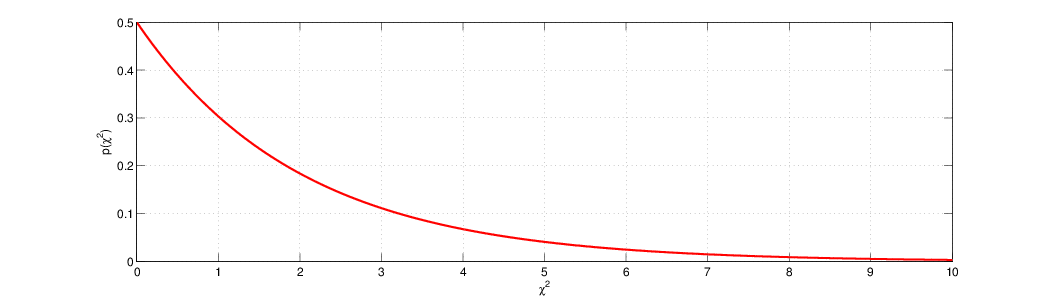
\includegraphics[width=0.7\textwidth]{chi22.png}
\end{frame}

\begin{frame}{Критерий согласия Пирсона}
%%%%%%%%%%%%%%%%%%%%%%%%%%%%%%%%%%%%%%%%%%%%%%%%%%%%%%%%%%%%%%%%%%%%%%%
% Статистика критерия конструируется следующим образом: область изменения случайной величины разбивается на K интервалов (карманов).
%Границы этих интервалов задаются величинами ai.
%Для каждого интервала [ai,ai+1] вычисляются две величины. Во-первых, ni — число элементов выборки, которое попало в интервал.
%Во-вторых, pi — теоретическая вероятность попадания в этот интервал при условии справедливости нулевой гипотезы. В данном случае это разность функций нормального распределения в точках ai+1 и ai
%%%%%%%%%%%%%%%%%%%%%%%%%%%%%%%%%%%%%%%%%%%%%%%%%%%%%%%%%%%%%%%%%%%%%%%
    \begin{itemize}
    \item Выборка: $X^n=\left(X_1,\ldots,X_n\right)$
    \item $H_0\colon X \sim N\left(\mu,\sigma^2\right)$,\qquad $H_1\colon \lnot H_0$
    \item Статистика: \alert{$\chi^2\left(X^n\right) = \sum_{i=1}^{K}\frac{(n_i-np_i)^2}{np_i}
    \sim \begin{cases}
        \chi^2_{K-1}, & \text{если $\mu,\sigma$ заданы}\\
        \chi^2_{K-3}, & \text{если $\mu,\sigma$ оцениваются}
        \end{cases}
    $}
    \item достигаемый уровень значимости:
    $p\left(\chi^2\right) = 1 - F_{\chi^2_{K-k-1}}\left(\chi^2\right)
    $
    \item  в Python \texttt{scipy.stats.shapiro(x)}
    \end{itemize}

    \bigskip
    \textbf{Недостатки:}
    \begin{itemize}
        \item разбиение на интервалы неоднозначно
        \item требует больших выборок ($np_i>5$ в~80\%~ячеек)
    \end{itemize}
\end{frame}

\begin{frame}{Критерии, основанные на эмпирической функции распределения}
\only<1>{
    Ряд критериев согласия основаны на различиях между $F\left(x\right)$ и $F_n\left(x\right)$:
    \begin{itemize}
        \item Джини: $$\int\left|F_n\left(x\right)-F\left(x\right)\right|dx$$
        \item Крамера-фон Мизеса: $$\int\left(F_n\left(x\right)-F\left(x\right)\right)^2dx$$
        \item Колмогорова (одновыборочный Колмогорова-Смирнова): $$\sup_{-\infty<x<\infty}\left|F_n\left(x\right)-F\left(x\right)\right|$$
        \item Смирнова-Крамера-фон Мизеса: $$\int\left(F_n\left(x\right)-F\left(x\right)\right)^2dF\left(x\right)$$
    \end{itemize}
}

\only<2>{
    \begin{itemize}
        \item Андерсона-Дарлинга: $$\int\frac{\left(F_n\left(x\right)-F\left(x\right)\right)^2}{F\left(x\right) \left(1-F\left(x\right)\right)}dF\left(x\right)$$
        \item Купера: $$\sup_{-\infty<x<\infty}\left(F_n\left(x\right)-F\left(x\right)\right) + \sup_{-\infty<x<\infty}\left(F\left(x\right)-F_n\left(x\right)\right)$$
        \item Ватсона: $$\int\left(F_n\left(x\right)-F\left(x\right) - \int \left(F_n\left(x\right)-F\left(x\right)\right)dF\left(x\right) \right)dF\left(x\right)$$
        \item Фроцини: $$\int\left|F_n\left(x\right)-F\left(x\right)\right|dF\left(x\right)$$
    \end{itemize}

    Предполагается, что $F\left(x\right)$ известна с точностью до параметров (если они оцениваются по выборке, нулевое распределение корректируется).
}
\end{frame}
\begin{frame}{Критерий Шапиро-Уилка}
%%%%%%%%%%%%%%%%%%%%%%%%%%%%%%%%%%%%%%%%%%%%%%%%%%%%%%%%%%%%%%%%%%%%%%%
% Статистика W рассчитывается на основании вариационного ряда, полученного из выборки, и некоторых величин a.
%Эти величины основаны на математических ожиданиях порядковых статистик из стандартного нормального распределения, они табулированы, для них не существует аналитических выражений.
%Кроме того, табулировано и нулевое распределение статистики критерия Шапиро-Уилка, то есть его невозможно записать аналитически.
%Используя таблицы этих величин, можно вычислить достигаемый уровень значимости.
%%%%%%%%%%%%%%%%%%%%%%%%%%%%%%%%%%%%%%%%%%%%%%%%%%%%%%%%%%%%%%%%%%%%%%%
\begin{itemize}
       \item  выборка:$X^n=\left(X_1,\ldots,X_n\right)$
       \item $H_0\colon X \sim N\left(\mu,\sigma^2\right)$,\qquad
        $H_1\colon \lnot H_0$
        \item Статистика:
        \begin{gather*}
            W \left(X^n\right) = \frac{\left(\sum\limits_{i=1}^n a_i X_{(i)}\right)^2}{\sum\limits_{i=1}^n\left(X_i-\bar{X}\right)^2}
            \\
            \left(a_1,\ldots,a_n\right) = \frac{m^TV^{-1}}{\left(m^TV^{-1}V^{-1}m\right)^{1/2}}
            \\
            m=\left(m_1,\ldots,m_n\right)^T~\text{математические ожидания порядковых статистик $N(0,1)$}, \\
            V \text{ --- их ковариационная матрица} \\
        \end{gather*}
        \item нулевое распределение:       табличное
        \item  в Python \alert{\texttt{scipy.stats.shapiro(x)}}
\end{itemize}
\end{frame}

\begin{frame}{О проверке нормальности}{Что не так в критериях?}
%%%%%%%%%%%%%%%%%%%%%%%%%%%%%%%%%%%%%%%%%%%%%%%%%%%%%%%%%%%%%%%%%%%%%%%
% Какой из рассмотренных критериев лучше использовать?
%%%%%%%%%%%%%%%%%%%%%%%%%%%%%%%%%%%%%%%%%%%%%%%%%%%%%%%%%%%%%%%%%%%%%%%
    \begin{itemize}
        \large
        \item \textbf{выбросы}: сильно влияют на выборочные коэффициенты асимметрии и эксцесса
        \bigskip
        \item \textbf{критерий Колмогорова}: представляет только исторический интерес
        \bigskip
        \item \textbf{критерий хи-квадрат}: слишком общий, не самый мощный, потеря информации из-за разбиения на интервалы
    \end{itemize}
\end{frame}

\begin{frame}{О проверке нормальности}{Какой критерий лучше?}
%%%%%%%%%%%%%%%%%%%%%%%%%%%%%%%%%%%%%%%%%%%%%%%%%%%%%%%%%%%%%%%%%%%%%%%
% В справочнике Кобзаря показано, что критерий Шапиро-Уилка обладает достаточно хорошей мощностью для разных классов альтернатив.
%%%%%%%%%%%%%%%%%%%%%%%%%%%%%%%%%%%%%%%%%%%%%%%%%%%%%%%%%%%%%%%%%%%%%%%
    \begin{center}
        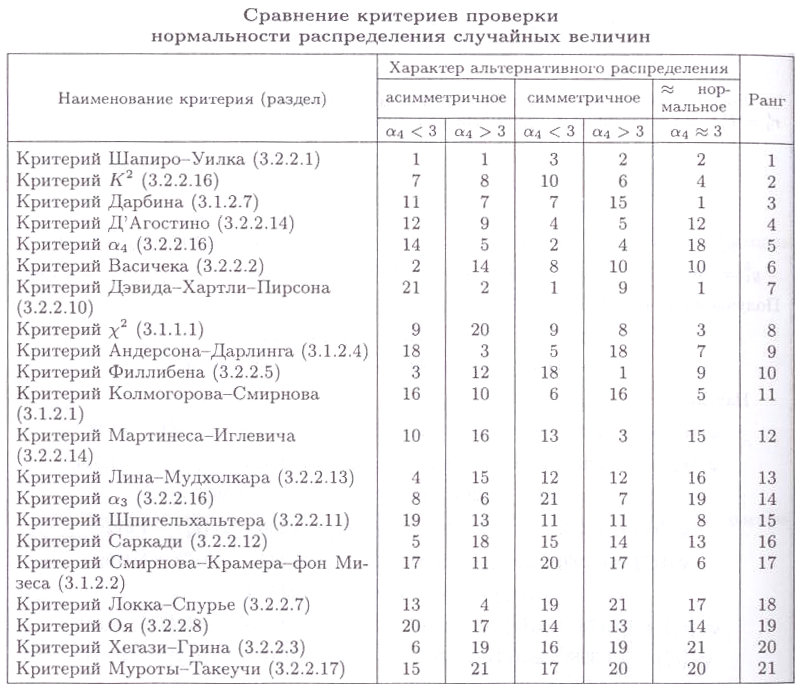
\includegraphics[height=0.8\textheight]{kobzar.png}
    \end{center}
    Кобзарь, 3.2.2.19, табл.~80.
\end{frame}

\begin{frame}{О проверке нормальности}{А нужно ли вообще?}

%%%%%%%%%%%%%%%%%%%%%%%%%%%%%%%%%%%%%%%%%%%%%%%%%%%%%%%%%%%%%%%%%%%%%%%
% Давайте сделаем шаг назад и подумаем, зачем нужно формально проверять нормальность.
% Дело в том, что проверка гипотезы нормальности наследует плохие свойства всего аппарата проверки гипотез: на маленьких выборках нулевая гипотеза, как правило, не отклоняется, а на выборках огромного размера — практически наверняка отклоняется. То есть, если выборка маленькая, то, формально проверяя гипотезу о нормальности, её не получается отклонить, а если выборка огромна, то гипотеза отклоняется, даже если распределение отличается от нормального совсем чуть-чуть.
% Многие методы, предполагающие нормальность, в том числе критерии Стьюдента, нечувствительны к небольшим отклонениям от нормальности, то есть истинное распределение выборки может слегка отличаться от нормального, и t-критерий будет всё еще правильно работать. Нормальное распределение — это математический конструкт. Никаких нормальных выборок в природе не существует. Однако, как говорил Джордж Бокс: «Все модели неверны, а некоторые полезны» — а нормальные модели очень полезны, поэтому их имеет смысл использовать.
%%%%%%%%%%%%%%%%%%%%%%%%%%%%%%%%%%%%%%%%%%%%%%%%%%%%%%%%%%%%%%%%%%%%%%%
\large
\begin{itemize}

    \item \textbf{очень маленькие выборки}: любой критерий может пропустить отклонения от нормальности, графические методы бесполезны
\bigskip
\item \textbf{очень большие выборки}
    \begin{itemize}
        \item любой критерий может выявлять небольшие статистически, но не практически значимые отклонения от нормальности;
        \item значительная часть методов, предполагающих нормальность, демонстрируют устойчивость к отклонениям от неё
    \end{itemize}
\end{itemize}
\end{frame}

\begin{frame}{О проверке нормальности}{так что же делать?}

%%%%%%%%%%%%%%%%%%%%%%%%%%%%%%%%%%%%%%%%%%%%%%%%%%%%%%%%%%%%%%%%%%%%%%%
% В итоге предлагается использовать следующий алгоритм.
%Если анализируемые данные имеют распределение, явно отличающееся от нормального (например, измеряемый признак — бинарный или категориальный), не нужно применять метод, предполагающий нормальность.
%Лучше использовать метод, специально разработанный для такого распределения.
%Если исследуемый признак, по крайней мере, измерен в непрерывной шкале, можно построить Q-Q график.
%Если на этом графике не видно существенных отклонений от нормальности (точки лежат примерно на прямой), можно использовать методы, устойчивые к небольшим отклонениям от нормальности, например, критерии Стьюдента.
%Если используемый метод чувствителен к отклонениям от нормальности, необходимо формально проверить нормальность, и рекомендуется это делать с помощью метода Шапиро-Уилка.
%Если критерий Шапиро-Уилка отвергает нормальность, не нужно использовать методы, чувствительные к отклонениям от нормальности.
%%%%%%%%%%%%%%%%%%%%%%%%%%%%%%%%%%%%%%%%%%%%%%%%%%%%%%%%%%%%%%%%%%%%%%%
    \large
    \begin{itemize}
        \item если  \textit{данные явно ненормальны} (например, бинарны или дискретны), нужно выбрать метод, специфичный для такого распределения
        \bigskip
        \item если \textit{на ку-ку графике не видно существенных отклонений от~нормальности}, можно сразу использовать методы, устойчивые к~небольшим отклонениям (например, критерии Стьюдента)
        \bigskip
        \item если метод  \textit{чувствителен к отклонениям от~нормальности} (например, критерий Фишера), проверять её рекомендуется критерием Шапиро-Уилка
        \bigskip
        \item если  \textit{нормальность отвергается}, чувствительные методы, предполагающие нормальность, использовать нельзя!
    \end{itemize}
\end{frame}


\section{Непараметрические критерии проверки гипотез}
\begin{frame}{}{}
    \centering
    \huge
    \bfseries
    Непараметрические критерии проверки гипотез
\end{frame}
%%%%%%%%%%%%%%%%%%%%%%%%%%%%%%%%%%%%%%%%%%%%%%%%%%%%%%%%%%%%%%%%%%%%%%%
%Теперь поговорим о непараметрических критериях. Непараметрические критерии применяются в задачах следующего типа.
%Есть выборка объема n из какого-то распределения F (x); проверяется гипотеза о равенстве чему-то среднего значения или дисперсии случайной величины, из которой взята эта выборка.
% Чтобы проверять любую гипотезу, нужна статистика, для которой должно быть известно нулевое распределение, то есть распределение при условии справедливости нулевой гипотезы.
%Если про исходное распределение F(x) что-то известно и T-статистика выбрана удачно, то нулевое распределение статистики может быть выражено аналитически. Однако распределение F(x) может быть нестандартным, и о нём может быть ничего не известно.
% Гипотезы про среднее значение можно проверять с использованием центральной предельной теоремы (фактически, с помощью Z-критерия).
%Но центральная предельная теорема не всегда применима: иногда распределения бывают слишком скошенные, иногда выборка недостаточно большая, чтобы распределение ее выборочного среднего можно было считать нормальным.
% В таких ситуациях существует два варианта действий.
%Во-первых, имеющуюся выборку из неизвестного распределения можно преобразовать так, что о её распределении будет больше информации.
%Во-вторых, можно сделать какие-то предположения о функции распределения исходной выборки F(x), и на основании этих предположений построить статистику, нулевое распределение которой можно оценить.
% В методах, которые будут рассмотрены далее, в разных комбинациях используются эти два способа работы с выборками.
%%%%%%%%%%%%%%%%%%%%%%%%%%%%%%%%%%%%%%%%%%%%%%%%%%%%%%%%%%%%%%%%%%%%%%%

\begin{frame}[label=classification]{Виды задач}
    \begin{itemize}
    \item Одновыборочные $X^n$:
    \begin{itemize}
        \item среднее выборки равно заданному числу \hyperlink{signtest1}{\beamerbutton{1}} \hyperlink{signrank1}{\beamerbutton{3}} \hyperlink{perm1s}{\beamerbutton{8}}
     \end{itemize}

     \bigskip

    \item Двухвыборочные {$X_1^{n_1}, X_2^{n_2}$}:
    \begin{itemize}
        \item среднее выборок равны
         \begin{itemize}
            \item $X_1$, $X_2$ связаны
            \hyperlink{signtest2}{\beamerbutton{2}} \hyperlink{signrank2}{\beamerbutton{4}}
            \item $X_1$, $X_2$ независимы
             \hyperlink{mannwhitney}{\beamerbutton{5}} \hyperlink{perm2sn}{\beamerbutton{10}}
         \end{itemize}
        \item дисперсии выборок равны
            \hyperlink{siegel}{\beamerbutton{6}}
            %\hyperlink{wm}{\beamerbutton{7}}
            \hyperlink{perm2d}{\beamerbutton{11}}
    \end{itemize}
    \end{itemize}
\end{frame}

\begin{frame}{Варианты двухвыборочных гипотез}
	 \begin{align*}
	 \intertext{О положении: }
	 H_0\colon &\mathbb{E} X_1 = \mathbb{E} X_2,              \;\;& \;\;H_1\colon &\mathbb{E} X_1 <\neq> \mathbb{E} X_2; \\
	 H_0\colon &\med X_1 = \med X_2,                          \;\;& \;\;H_1\colon &\med X_1 <\neq> \med X_2; \\
	 H_0\colon &\prob\left( X_1 > X_2\right)=0.5,           \;\;& \;\;H_1\colon &\prob\left( X_1 > X_2\right) <\neq> 0.5; \\
	 H_0\colon &F_{X_1}\left(x\right) = F_{X_2}\left(x\right),\;\;& \;\;H_1\colon &F_{X_1}\left(x\right) = F_{X_2}\left(x+\Delta\right), \Delta <\neq> 0; \\
	 H_0\colon &F_{X_1}\left(x\right) = F_{X_2}\left(x\right),\;\;& \;\;H_1\colon &F_{X_1}\left(x\right)  <\neq> F_{X_2}\left(x\right). \\
	 \intertext{О рассеянии: }
	 H_0\colon &\mathbb{D} X_1 = \mathbb{D} X_2,                     \;\; & \;\;H_1\colon &\mathbb{D} X_1 <\neq> \mathbb{D} X_2; \\
	%    H_0\colon &\mathbb{D} X_1 = \mathbb{D} X_2, \med X_1=\med X_2,  \;\; & \;\;H_1\colon &\mathbb{D} X_1 <\neq> \mathbb{D} X_2; \\
	 H_0\colon &F_{X_1}\left(x\right) = F_{X_2}\left(x+\Delta\right),\;\; & \;\;H_1\colon & F_{X_1}\left(x\right) = F_{X_2}\left(\sigma x+\Delta\right), \sigma <\neq> 1.
	 \end{align*}
\end{frame}

\section{Знаки}
\subsection{Одна выборка}

\begin{frame}{Биномиальный критерий}
	\begin{center}
		\begin{tabular}{rl}
			выборка:                        & $X^{n}=\left(X_{1},\ldots,X_{n}\right), X \sim Ber\left(p\right)$ \\
			нулевая гипотеза:               & $H_0\colon p=p_0$ \\
			альтернатива:                   & $H_1\colon p \gtrless p_0$ \\
			статистика:                     & $T\left(X^{n}\right) = \sum\limits_{i=1}^n X_i \sim Bin(n,p_0)$ \\
		\end{tabular}
		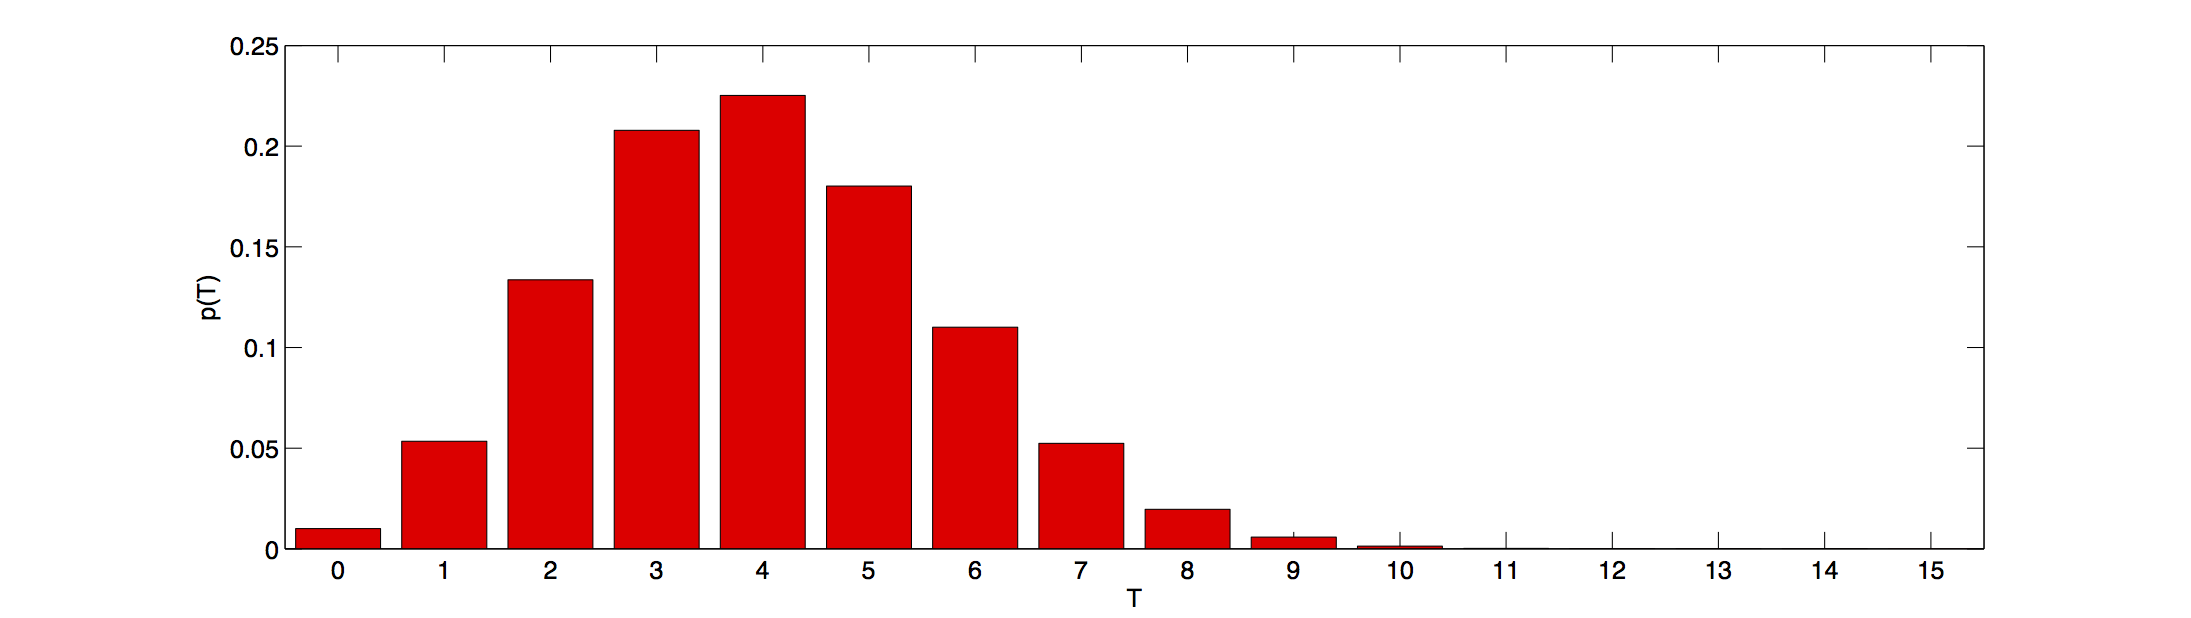
\includegraphics[width=0.6\textwidth]{bin_nonsym.png}
	\end{center}

	\vspace{-5pt}
	% -1 здесь из-за дискретности. Если аккуратно все посчитать - выходит действительно, что нужно вычесть единицу
	достигаемый уровень значимости:
	$$p\left(T\right) = \begin{cases}
	1-F_{Bin(n,p_0)}(T-1), & H_1 \colon p>p_0, \\
	F_{Bin(n,p_0)}(T),   & H_1 \colon p<p_0, \\
%	\text{через бета-распределение},       & H_1 \colon p\neq p_0. \\
	\end{cases}
	$$

\end{frame}


\begin{frame}[label=signtest1]{\hyperlink{classification}{\beamerbutton{(1)}} Одновыборочный критерий знаков}
%%%%%%%%%%%%%%%%%%%%%%%%%%%%%%%%%%%%%%%%%%%%%%%%%%%%%%%%%%%%%%%%%%%%%%%
% Критерии знаков — это одно из семейств непараметрических критериев. Эти критерии обладают невысокой мощностью, но они крайне универсальны и практически ничего не требуют от данных, поэтому они очень полезны на практике.
%%%%%%%%%%%%%%%%%%%%%%%%%%%%%%%%%%%%%%%%%%%%%%%%%%%%%%%%%%%%%%%%%%%%%%%
 \begin{center}
     \begin{tabular}{rl}
         выборка:                        & $X^n=\left(X_1,\ldots,X_n\right), X_i \neq m_0$         \\
         нулевая гипотеза:               & $H_0\colon \med X = m_0$ \\
         альтернатива:                   & $H_1\colon \med X \gtrless m_0$ \\
         статистика:                     & $T\left(X^n\right) = \sum\limits_{i=1}^n \left[X_i>m_0\right]$\\
         нулевое распределение:          & $Bin(n,\frac1{2})$\\
     \end{tabular}
     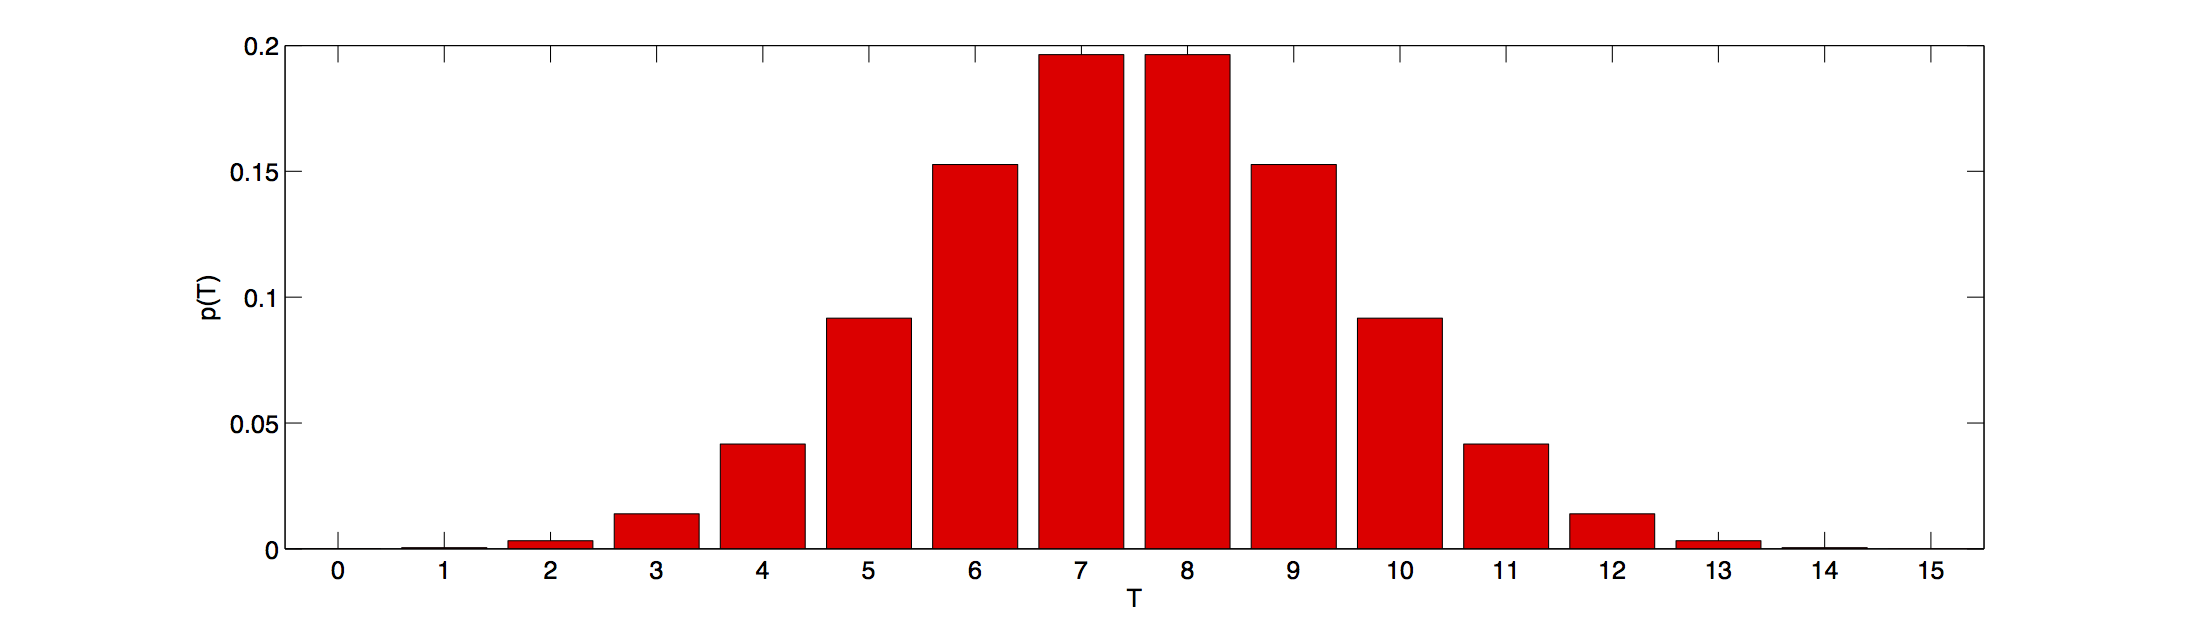
\includegraphics[width=0.8\textwidth]{bin.png}
 \end{center}
\end{frame}


\begin{frame}{Пример: одновыборочный критерий знаков}%%%%%%%%%%%%%%%%%%%%%%%%%%%%%%%%%%%%%%%%%%%%%%%%%%%%%%%%%%%%%%%%%%%%%%%
%Критерий знаков настолько нетребователен к данным, что его можно использовать даже на цензурированных выборках.
% Пример. Наблюдаются пациенты с лимфоцитарной лимфомой, измеряемый признак — это время их жизни в неделях после того, как был поставлен диагноз. Исследование длится семь лет. В выборке есть один пациент, который после семи лет (362 недель наблюдений) остался жив. Поскольку исследование закончи- лось, неизвестно, сколько еще он прожил после этого. Такая выборка называется цензурированной сверху, поскольку на части объектов известна только нижняя граница значения признака.
% Если требуется проверить гипотезу о том, что среднее время дожития составляет 200 недель, против односторонней альтернативы, что оно больше 200 недель, для этой выборки можно без проблем использовать критерий знаков. Его достигаемый уровень значимости p = 0.9453. То есть нулевую гипотезу нельзя отклонить против односторонней альтернативы.
%%%%%%%%%%%%%%%%%%%%%%%%%%%%%%%%%%%%%%%%%%%%%%%%%%%%%%%%%%%%%%%%%%%%%%%
\begin{block}{ Dinse, 1982}
Выживаемость пациентов с лимфоцитарной лимфомой (в~неделях):
 $$49, 58, 75, 110, 112, 132, 151, 276, 281, 362^*$$
 Исследование длилось 7 лет, поэтому для пациентов, проживших дольше, выживаемость неизвестна (выборка цензурирована сверху).

 Превышает ли среднее время дожития 200 недель?
 \end{block}
 \bigskip
\begin{itemize}
   \item $H_0\colon$ медиана времени дожития не отличается от 200 недель.

   \item $H_1\colon$ медиана времени дожития больше 200 недель.

   \item $T\left(X^n\right) = \sum\limits_{i=1}^n \left[X_i>200\right] = 3$

  \item
    $F_{Bin(10,1/2)}(3)
    =C_{10}^0\frac{1}{2^{10}}
    +C_{10}^1\frac{1}{2^{10}}
        +C_{10}^2\frac{1}{2^{10}} \sum() \approx 0.0547$

  ~\hfill \alert{\texttt{scipy.stats.binom(10,1/2).cdf(2)}}

   \item Критерий знаков: $p =1-0.0547 \approx 0.9453$.
\end{itemize}
\end{frame}


\subsection{Две выборки}
%%%%%%%%%%%%%%%%%%%%%%%%%%%%%%%%%%%%%%%%%%%%%%%%%%%%%%%%%%%%%%%%%%%%%%%
% В этом уроке идёт речь о непараметрических критериях, которые проверяют гипотезы о средних, но под «средними» они часто понимают совершенно разные вещи. Так, одновыборочный критерий знаков под средним понимает медиану. Двухвыборочный критерий знаков гипотезу о средних формулирует в представленном выше экзотическом виде. Другие критерии могут использовать другие варианты нулевых гипотез, но, тем не менее, всё это — в каком-то виде утверждение о средних.
% Пример с тополями – тополи использовались для очистки почвы от загрязнения на месте бывшей свалки. Наименьшая концентрация тяжелых металлов была обнаружена в дереве / коре, наибольшая – в листьях старых деревьев -> уборка листьев обязательна :) Сделан вывод, что концентрация тяжелых металлов не влияет на количество древесины.
%%%%%%%%%%%%%%%%%%%%%%%%%%%%%%%%%%%%%%%%%%%%%%%%%%%%%%%%%%%%%%%%%%%%%%%
\begin{frame}[label=signtest2]{\hyperlink{classification}{\beamerbutton{(2)}} Двухвыборочный критерий знаков}
 \only<1>{
 \begin{center}
    \begin{tabular}{rl}
         выборки:                        & $X_1^n=\left(X_{11},\ldots,X_{1n}\right)$\\
                                         & $X_2^n=\left(X_{21},\ldots,X_{2n}\right), X_{1i} \neq X_{2i}$ \\
                                         & выборки связанные\\
         нулевая гипотеза:               & $H_0\colon \prob\left( X_{1} > X_{2}\right) = \frac1{2}$ \\
         альтернатива:                   & $H_1\colon \prob\left( X_{1} > X_{2}\right) <\neq> \frac1{2}$ \\
         статистика:                     & $T\left(X_1^n, X_2^n\right) = \sum\limits_{i=1}^n \left[X_{1i}>X_{2i}\right]$ \\
         нулевое распределение:          & $Bin(n,\frac1{2})$\\
    \end{tabular}
    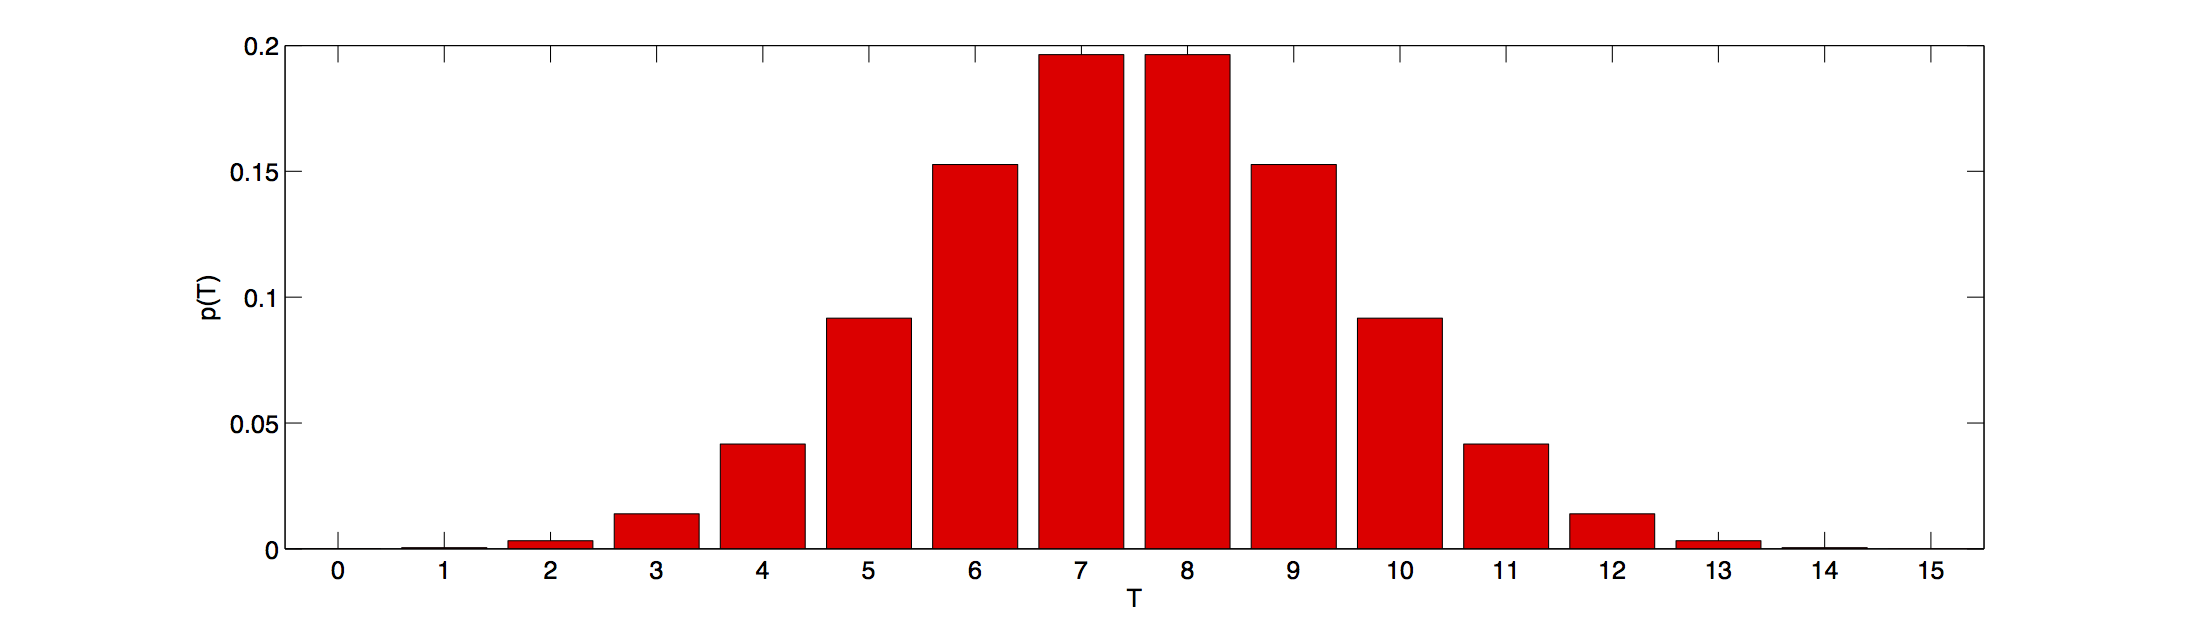
\includegraphics[width=0.8\textwidth]{bin.png}
 \end{center}
 }

 \only<2>{
\begin{block}{Пример, Hollander \& Wolfie, 29f}
 Депрессивность 9~пациентов была измерена по шкале Гамильтона до и после первого приёма транквилизатора. Подействовал ли транквилизатор?
 \end{block}
\begin{columns}
\begin{column}{0.4\textwidth}
 \begin{figure}
		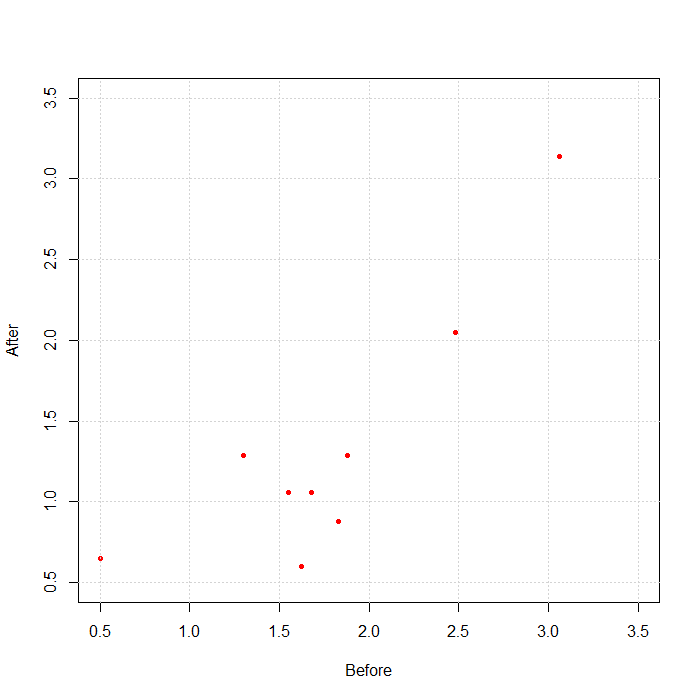
\includegraphics[width=0.8\textwidth]{hamilton.png}
 \end{figure}
    \end{column}
\begin{column}{0.35\textwidth}
$H_0\colon$ уровень депрессивности не изменился.

 $H_1\colon$ уровень депрессивности снизился.

 	\bigskip

 Критерий знаков: $p = 0.09$, 95\% нижний доверительный предел для медианы изменения~--- $-0.041$.
\end{column}
\end{columns}
	}

	\only<3>{
	\begin{block}{Пример, Laureysens et al., 2004} Для 13 разновидностей тополей, растущих в зоне интенсивного загрязнения, в августе и ноябре измерялась средняя концентрация алюминия в микрограммах на грамм древесины.
	\end{block}
\begin{columns}
\begin{column}{0.35\textwidth}
 \begin{figure}
		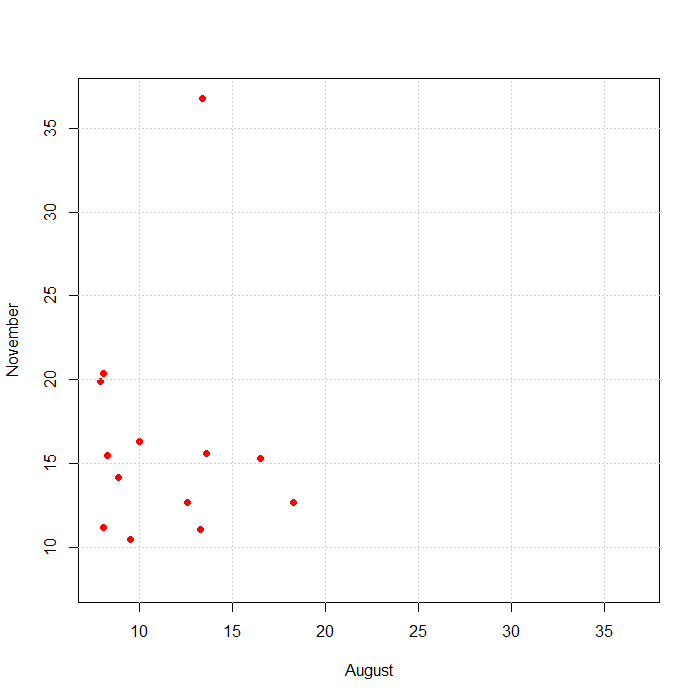
\includegraphics[width=0.8\textwidth]{poplar.png}
 \end{figure}
   \end{column}
\begin{column}{0.55\textwidth}
	$H_0\colon$ концентрация алюминия не менялась.

		$H_1\colon$ концентрация алюминия изменилась.


	Для тополей 10 из 13 разновидностей концентрация алюминия увеличилась.

	Критерий знаков: $p=0.0923$,

    95\% доверительный интервал для медианы изменения: $\left[-0.687, 10.107\right].$
   \end{column}
   \end{columns}
	}

\end{frame}



%%%%%%%%%%%%%%%%%%%%%%%%%%%%%%%%%%%%%%%%%%%%%	%%%%%%%%%%%%%%%%%%%%%%%%%%
% первый пример про комаров --- это когда ты тестируешь эффективность двух репеллентов, намазываешь одних и тех же людей каждым по очереди, выставляешь их в тундру, а потом спрашиваешь, когда они больше страдали
% третий пример про медь – подавляет ли кусок меди в пруду развитие личинок комаров: количество личинок комаров - очень шумная переменная с большой дисперсией, используя критерий знаков, можно искусственно снизить влияние дисперсии на вывод
%%%%%%%%%%%%%%%%%%%%%%%%%%%%%%%%%%%%%%%%%%%%%%%%%%%%%%%%%%%%%%%%%%%%%%%

\begin{frame}{Причины использовать критерий знаков}
 \begin{itemize}
     \item Точные разности $\Delta x_i$ неизвестны, известны только их знаки (сравнение агрессивности комаров).
     \bigskip
     \item Разности $\Delta x_i$ при $H_1$ могут быть небольшими по модулю, но иметь систематический характер по знаку (пример с мышами).
     \bigskip
     \item Разности $\Delta x_i$ при $H_0$ могут быть большими по модулю, но случайными но знаку (влияние меди на число личинок комаров).
     \bigskip
 \end{itemize}
\end{frame}



\section{Ранги}
%%%%%%%%%%%%%%%%%%%%%%%%%%%%%%%%%%%%%%%%%%%%%%%%%%%%%%%%%%%%%%%%%%%%%%%
% Для проверки гипотез о средних критерии знаков выбрасывают большую часть информации, содержащуюся в выборке.
%Вместо исходных значений признака используется бинарный вектор.
%Ранговые критерии позволяют сохранить больше информации.
% Обратить внимание студентов на дополнительное предположение о симметричности в отличие от критерия знаков --> отсюда возможность отвергнуть нулевую гиптезу из-за несимметричности распределения, а не из-за отличий медианы => дополнительно необходимо проверять семметричность
% Дополнительный плюс методов – можно использовать не только для числовых, но и для ordinal scales, поскольку тествая статистика зависит только от знака и ранга (более экзотично, но тем не менее полезно)
%%%%%%%%%%%%%%%%%%%%%%%%%%%%%%%%%%%%%%%%%%%%%%%%%%%%%%%%%%%%%%%%%%%%%%%
\begin{frame}{Вариационный ряд, ранги, связки}
 $$X_1,\ldots,X_n \;\;\; \Rightarrow \;\;\; X_{(1)}\leq\ldots < \underbrace{X_{(k_1)} = \ldots = X_{(k_2)}}_{\text{связка размера } k_2-k_1+1}<\ldots\leqslant  X_{(n)}$$

 \bigskip

 \structure{Ранг} наблюдения $X_i$:
%    $$\rank\left(X_i\right)=\mathbb{E}\left\{r\left|X_i=X_{(r)}\right.\right\}$$
%    т.\,е.
   \begin{itemize}
    \item если $X_i$ не в связке, то $\rank\left(X_i\right)=r\colon X_i=X_{(r)}$,
    \item если $X_i$ в связке $X_{(k_1)}, \ldots, X_{(k_2)}$, то $\rank\left(X_i\right)=\frac{k_1+k_2}{2}.$
   \end{itemize}
\end{frame}

\subsection{Одна выборка}
\begin{frame}[label=signrank1]{\hyperlink{classification}{\beamerbutton{(3)}} Одновыборочный критерий знаковых рангов Уилкоксона}
 \only<1>{
   \begin{center}
     \begin{tabular}{rl}
         выборка:                        & $X^n=\left(X_1,\ldots,X_n\right), X_i \neq m_0$\\
					            & $F\left(X\right)$ симметрично относительно медианы\\
         нулевая гипотеза:               & $H_0\colon \med X = m_0$ \\
         альтернатива:                   & $H_1\colon \med X <\neq> m_0$ \\
         статистика:                     & $W\left(X^n\right) = \sum\limits_{i=1}^n \rank\left(\left|X_i - m_0\right|\right)\cdot \sign\left(X_i - m_0\right)$ \\
         нулевое распределение:          & табличное\\
         в Python:          & \texttt{scipy.stats.wilcoxon(d)}\\
         \end{tabular}
     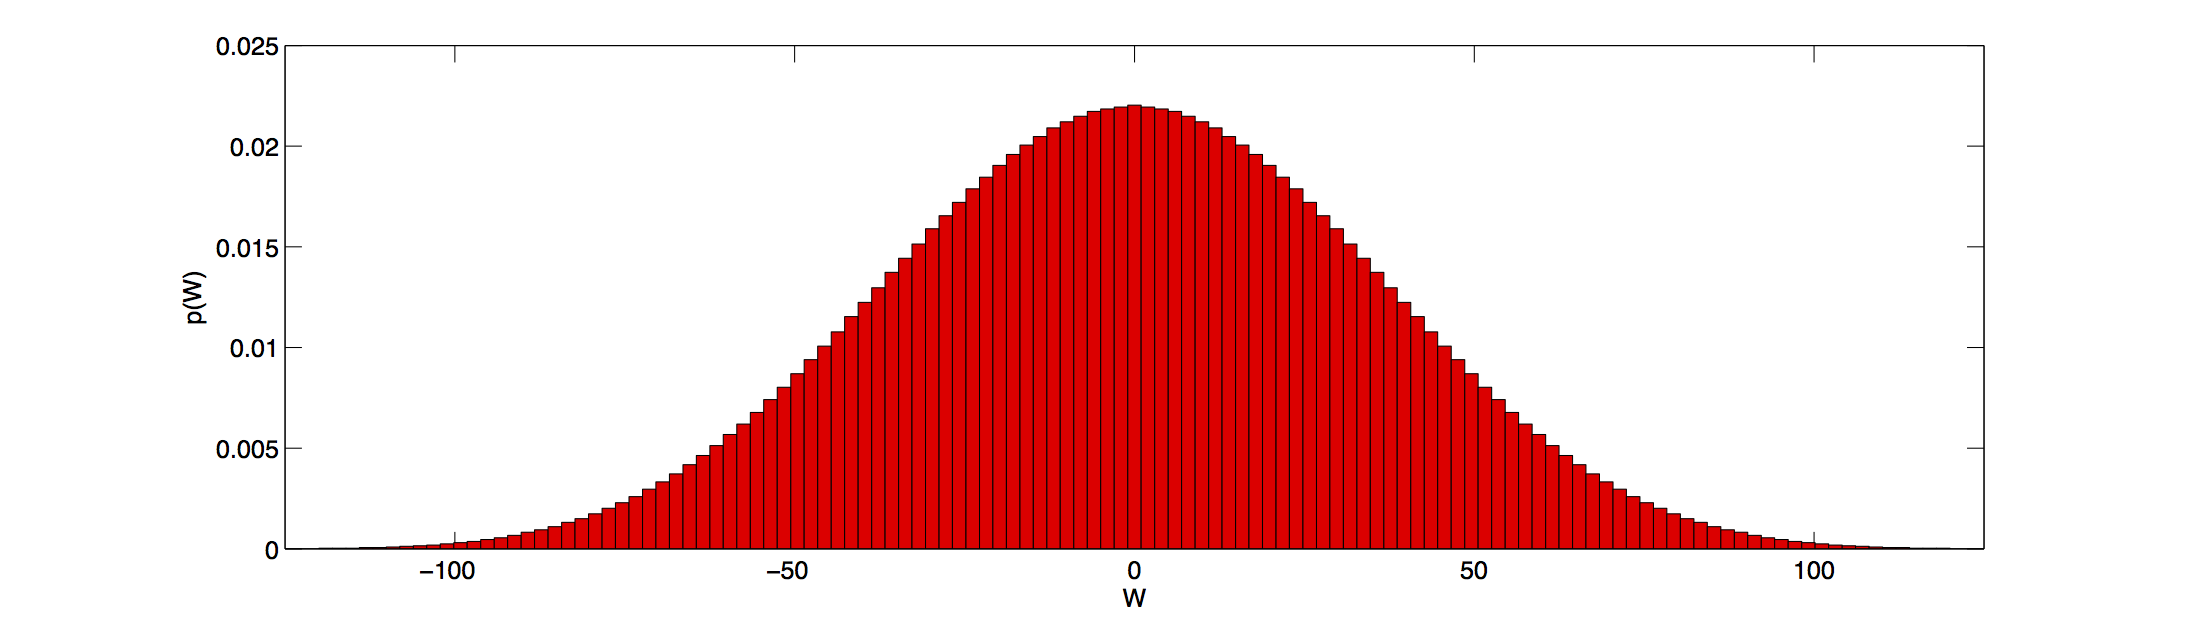
\includegraphics[width=0.8\textwidth]{signrank.png}
 \end{center}
 }

 \only<2>{
%%%%%%%%%%%%%%%%%%%%%%%%%%%%%%%%%%%%%%%%%%%%%%%%%%%%%%%%%%%%%%%%%%%%%%%
% При справедливости нулевой гипотезы каждый из рангов в выборке мог с одинаковой вероятностью реализоваться с любым знаком (sign(Xi ? m0)): и с «+», и с «-». Таким образом, получается 2n вариантов распределения знаков по рангам. Перебирая все эти варианты, для каждого из них можно вычислить значение статистики, пример перебора показан в таблице. Именно так строится нулевое распределение критерия знаковых рангов.
%%%%%%%%%%%%%%%%%%%%%%%%%%%%%%%%%%%%%%%%%%%%%%%%%%%%%%%%%%%%%%%%%%%%%%%
 Откуда берётся табличное распределениё

 \bigskip

    \begin{center}  \setlength{\tabcolsep}{5pt}
        \begin{tabular}{c c c c c c c c c c c}
        $1$&$2$&$3$&$4$&$5$&$W$\\
        $-$&$-$&$-$&$-$&$-$&$-15$\\
        $+$&$-$&$-$&$-$&$-$&$-13$\\
        $-$&$+$&$-$&$-$&$-$&$-11$\\
        $+$&$+$&$-$&$-$&$-$&$-9$\\
        $-$&$-$&$+$&$-$&$-$&$-9$\\
        \dots&\dots&\dots&\dots&\dots&\dots\\
         $+$&$+$&$-$&$+$&$+$&$9$\\
        $-$&$-$&$+$&$+$&$+$&$9$\\
        $+$&$-$&$+$&$+$&$+$&$11$\\
        $-$&$+$&$+$&$+$&$+$&$13$\\
        $+$&$+$&$+$&$+$&$+$&$15$\\
        \end{tabular}
    \end{center}

    Всего $2^n$ вариантов.
 }
    \only<3>{
    $n=5$:

    \begin{center}
        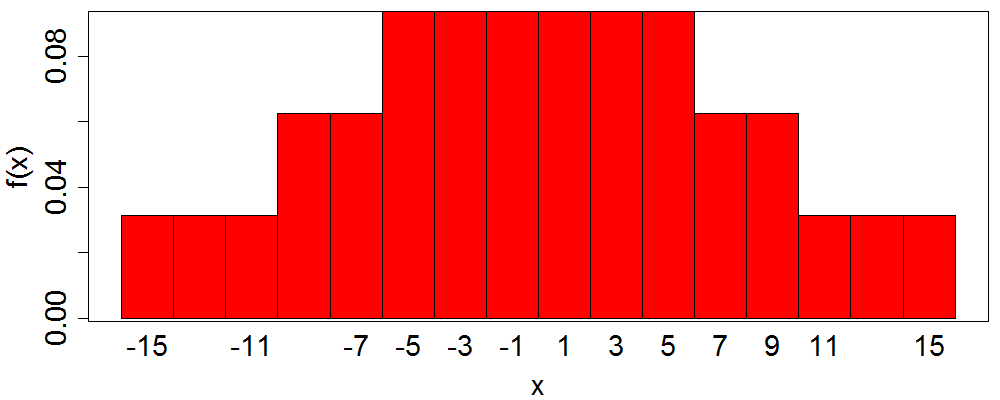
\includegraphics[width=0.8\textwidth]{ranksum5.png}
    \end{center}
    }
    \only<4>{
    $n=10$:

    \begin{center}
        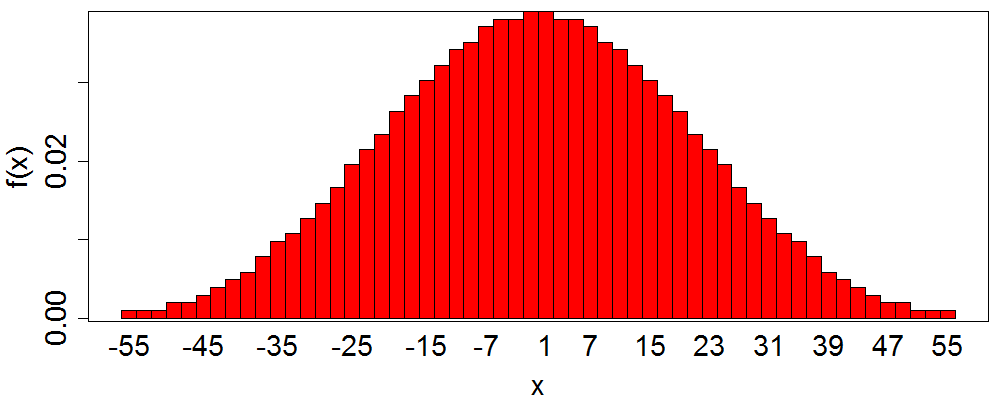
\includegraphics[width=0.8\textwidth]{ranksum10.png}
    \end{center}
    }
\only<5>{
    $n=15$:

    \begin{center}
        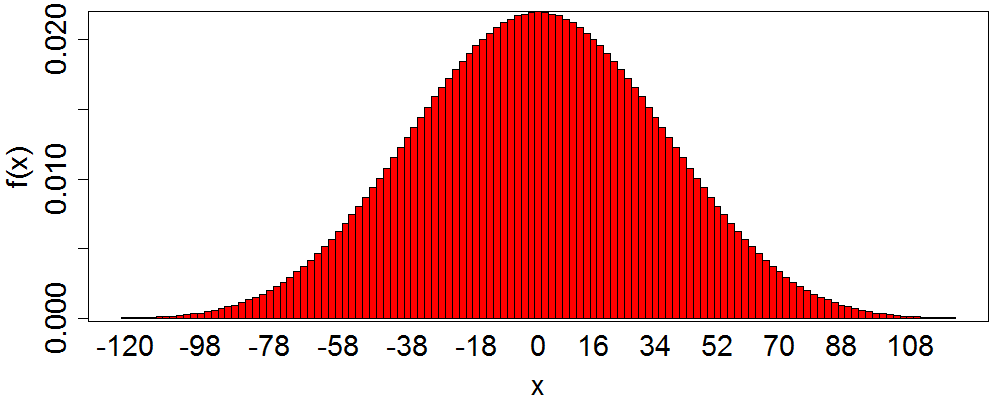
\includegraphics[width=0.8\textwidth]{ranksum15.png}
    \end{center}

    \bigskip

    Аппроксимация для $n>20$:
    $$W\approx \sim N\left(0, \frac{n(n+1)(2n+1)}{6}\right).$$
    }
 \only<6>{
 \textbf{Пример 1} (Bonnini, табл. 1.4): диаметры шайб на производстве ($n=24$):

     \begin{center}
         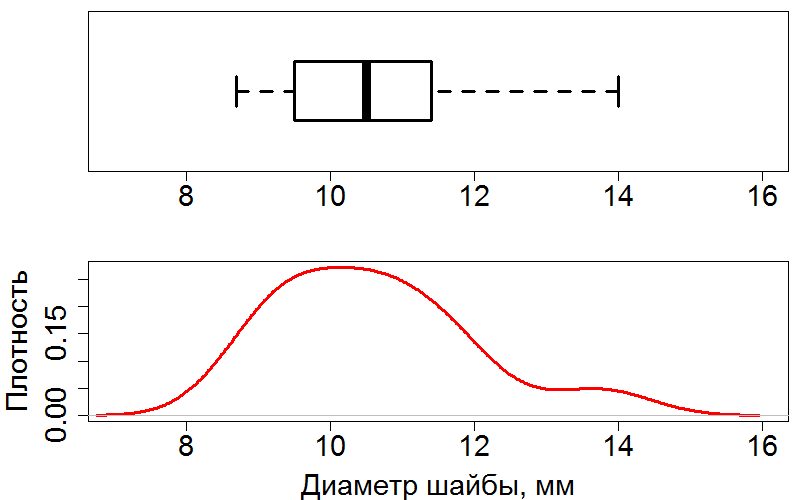
\includegraphics[width=0.4\textwidth]{washer.png}
     \end{center}

     Соответствуют ли шайбы стандартному размеру 10 мм?

 \bigskip

	$H_0\colon$ средний диаметр шайбы~--- $10$ мм, $\med X = 10$.

	$H_1\colon$ средний диаметр шайбы не соответствует стандарту, $\med X\neq10$.

	\bigskip

	Критерий знаковых рангов: $p=0.0673$, выборочная медиана диаметра~--- $10.5$~мм ($95$\% доверительный интервал~---  $\left[9.95, 11.15\right]$~мм).
 }

% \only<7>{
% \textbf{Пример 2} (зеркала в клетках мышей):\\
% \bigskip
%
% $H_0\colon$ медиана доли времени, проводимого в клетке с зеркалом, равна~$\frac{1}{2}.$
%
% $H_1\colon$ медиана доли времени, проводимого в клетке с зеркалом, не~равна~$\frac{1}{2}$.
%
%  \bigskip
%  Критерий знаковых рангов: $p=0.0934.$
% }
\end{frame}

\subsection{Две выборки}
\begin{frame}[label=signrank2]{\hyperlink{classification}{\beamerbutton{(4)}} Критерий знаковых рангов Уилкоксона для связанных выборок}
%%%%%%%%%%%%%%%%%%%%%%%%%%%%%%%%%%%%%%%%%%%%%%%%%%%%%%%%%%%%%%%%%%%%%%%
% Как и до этого в курсе, двухвыборочная задача со связанными выборками решается с использованием того же самого критерия, что и одновыборочная.
%%%%%%%%%%%%%%%%%%%%%%%%%%%%%%%%%%%%%%%%%%%%%%%%%%%%%%%%%%%%%%%%%%%%%%%
 \only<1>{
   \begin{center}
     \begin{tabular}{rl}
         выборки:                        & $X_1^n=\left(X_{11},\ldots,X_{1n}\right)$         \\
                                         & $X_2^n=\left(X_{21},\ldots,X_{2n}\right), X_{1i} \neq X_{2i}$ \\
                                         & выборки связанные, разность выборок симметрична относительно медианы\\
         нулевая гипотеза:               & $H_0\colon \med \left(X_{1} - X_{2}\right)=0$ \\
         альтернатива:                   & $H_1\colon \med \left(X_{1} - X_{2}\right) <\neq> 0$ \\
         статистика:                     & $W\!\left(X_1^n, X_2^n\right)\! = \!\!\sum\limits_{i=1}^n \!\rank\!\left(\left|X_{1i} - X_{2i}\right|\right)\cdot \sign\!\left(X_{1i} - X_{2i}\right)$ \\
         нулевое распределение:          & табличное\\
     \end{tabular}
     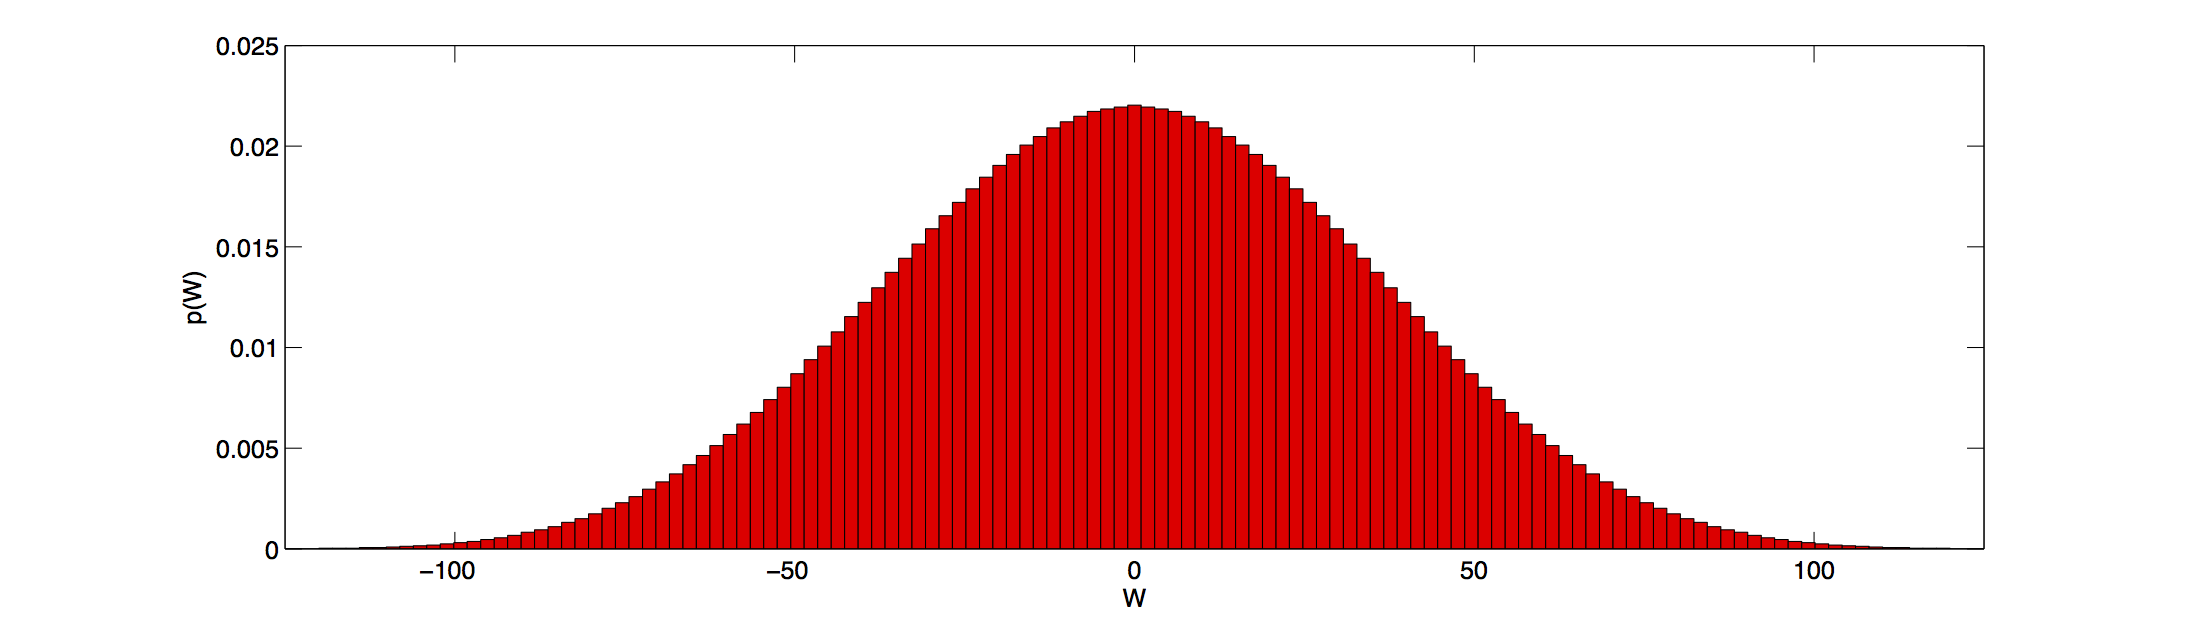
\includegraphics[width=0.8\textwidth]{signrank.png}
 \end{center}
 }

 \only<2>{
 \begin{block}{Пример, Kanji, критерий 48} Управляемый вручную станок на каждом шаге процесса производит пару пружин. Для 14~пар измерена прочность:
 \begin{align*}
 X_1\colon & \{1.38,  0.39, 1.42, 0.54, 5.94, 0.59, 2.67, 2.44, 0.56, 0.69, 0.71, 0.95, 0.50, 9.69\}, \\
 X_2\colon & \{1.42, 0.39, 1.46, 0.55, 6.15, 0.61, 2.69, 2.68, 0.53, 0.72, 0.72, 0.93, 0.53, 10.37\}.
 \end{align*}
 Одинакова ли прочность пружин в парё
 \end{block}
 \bigskip

 $H_0\colon$ средние значение прочности пружин в паре равны.

 $H_1\colon$ средние значение прочности пружин в паре не равны $ \Rightarrow p = 0.0142$, 95\% доверительный интервал для медианной разности~--- $\left[0.005, 0.14\right].$
 }
%
% \only<3>{
% \textbf{Пример 2} (алюминий в тополях):\\
% \bigskip
%
% $H_0\colon$ медиана изменения концентрации алюминия равна нулю.
%
% $H_1\colon$ медиана изменения концентрации алюминия не~равна нулю $\Rightarrow 0.0398,$ 95\% доверительный интервал для медианы изменения~--- $\left[0.35, 9.3\right].$
% }
\end{frame}

\begin{frame}[label=mannwhitney]{\hyperlink{classification}{\beamerbutton{(5)}} Критерий Манна-Уитни-Уилкоксона}
 \only<1>{
%%%%%%%%%%%%%%%%%%%%%%%%%%%%%%%%%%%%%%%%%%%%%%%%%%%%%%%%%%%%%%%%%%%%%%%
% Относительно параметра ? альтернатива в этом критерии может быть односторонней или двусторонней. Если справедлива альтернативная гипотеза и между распределениями действительно есть сдвиг, то средние значения признаков в выборках будут различаться. Поэтому это тоже в каком-то виде гипотеза о средних.
%%%%%%%%%%%%%%%%%%%%%%%%%%%%%%%%%%%%%%%%%%%%%%%%%%%%%%%%%%%%%%%%%%%%%%%
   \begin{center}
     \begin{tabular}{rl}
         выборки:                        & $X_1^{n_1}=\left(X_{11},\ldots,X_{1n_1}\right)$         \\
                                         & $X_2^{n_2} = \left(X_{21},\ldots,X_{2n_2}\right)$ \\
                                         & выборки независимые\\
         нулевая гипотеза:               & $H_0\colon F_{X_1}\left(x\right) = F_{X_2}\left(x\right)$ \\
         альтернатива:                   & $H_1\colon F_{X_1}\left(x\right) = F_{X_2}\left(x+\Delta\right), \Delta <\neq> 0$ \\
         статистика:                     & $X_{(1)}\leq\ldots\leqslant  X_{(n_1+n_2)}$ --- вариационный ряд \\
                                         & объединённой выборки $X = X_1^{n_1} \bigcup X_2^{n_2}$ \\
                                         & $R_1\left(X_1^{n_1}, X_2^{n_2}\right) = \sum\limits_{i=1}^{n_1} \rank\left(X_{1i}\right)$ \\
         нулевое распределение:          & табличное\\
         в Python: & \alert{\texttt{scipy.stats.mannwhitneyu(x1, x2)}}\\
     \end{tabular}
     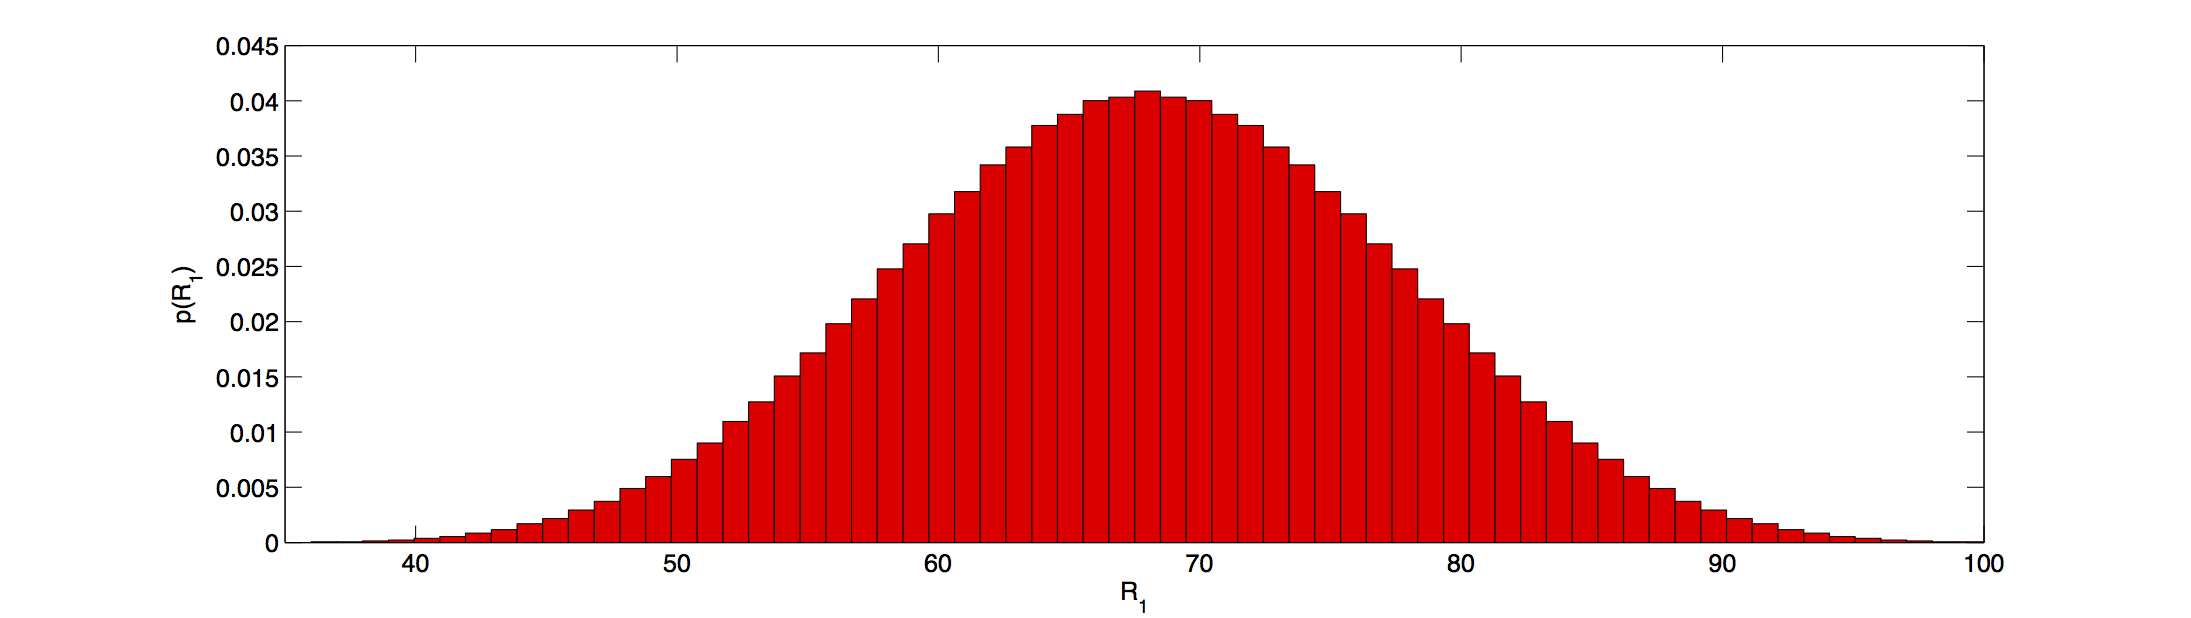
\includegraphics[width=0.7\textwidth]{mann.png}
 \end{center}
 }
 \only<2>{
%%%%%%%%%%%%%%%%%%%%%%%%%%%%%%%%%%%%%%%%%%%%%%%%%%%%%%%%%%%%%%%%%%%%%%%
% Нулевое распределение этой статистики, как и в предыдущем случае, табличное. Оно получается следующим образом. Если нулевая гипотеза справедлива, то каждый из рангов с одинаковой вероятностью мог реализоваться как в выборке X1, так и в выборке X2. Необходимо перебрать все возможные варианты того, как это могло произойти, всего таких вариантов n1. На каждом из этих вариантов нужно вычислить n1+n2 значение статистики критерия Манни-Уитни, так и получается нулевое распределение.
%%%%%%%%%%%%%%%%%%%%%%%%%%%%%%%%%%%%%%%%%%%%%%%%%%%%%%%%%%%%%%%%%%%%%%%
 Откуда берётся табличное распределение?


    \begin{center}
    	\begin{tabular}{c c c}
    		$X_1$ & $X_2$  & $R_1$\\
    		\{1,2,3\}      & \{4,5,6,7\}     & 6 \\
    		\{1,2,4\}      & \{3,5,6,7\}     & 7 \\
    		\{1,2,5\}      & \{3,4,6,7\}     & 8 \\
    		\{1,2,6\}      & \{3,4,5,7\}     & 9 \\
    		\{1,2,7\}      & \{3,4,5,6\}     & 10 \\
    		\{1,3,4\}      & \{2,5,6,7\}     & 8 \\
    		\dots&\dots&\dots\\
    		\{3,5,7\}      & \{1,2,4,6\}     & 15 \\
    		\{3,6,7\}      & \{1,2,4,5\}     & 16 \\
    		\{4,5,6\}      & \{1,2,3,7\}     & 15 \\
    		\{4,5,7\}      & \{1,2,3,6\}     & 16 \\
    		\{4,6,7\}      & \{1,2,3,5\}     & 17 \\
    		\{5,6,7\}      & \{1,2,3,4\}     & 18 \\
    	\end{tabular}
    \end{center}

    Всего $C_{n_1+n_2}^{n_1}$ вариантов.
 }

   \only<3>{
    	$n_1=n_2=5$:

    	\begin{center}
    		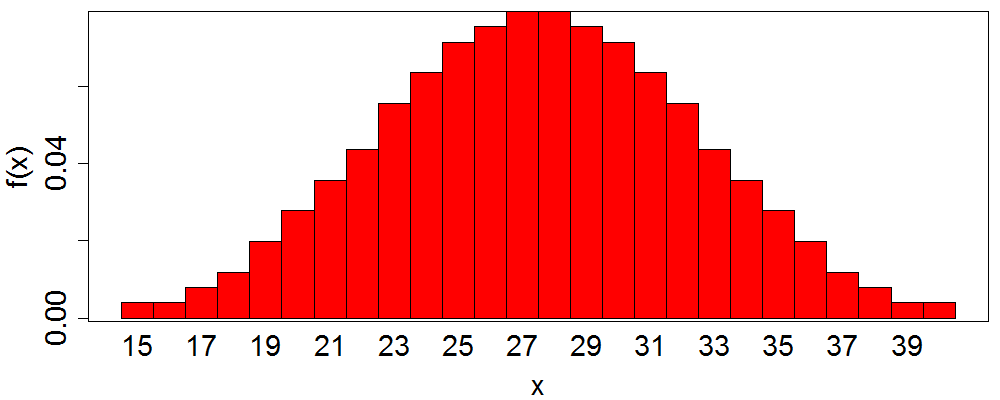
\includegraphics[width=0.8\textwidth]{MU5-5.png}
    	\end{center}
    }
    \only<4>{
    	$n_1=n_2=10$:

    	\begin{center}
    		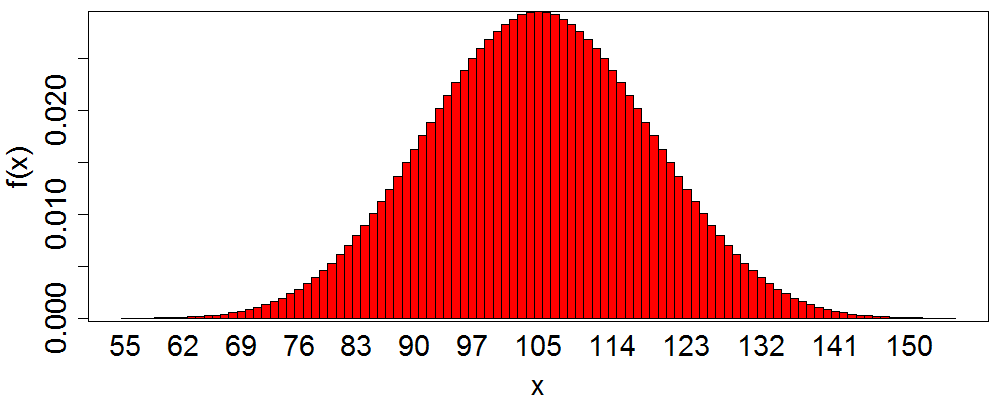
\includegraphics[width=0.8\textwidth]{MU10-10.png}
    	\end{center}

    	\bigskip

    	Аппроксимация для $n_1,n_2>10$:
    	$$R_1\sim N\left(\frac{n_1(n_1+n_2+1)}{2}, \frac{n_1n_2(n_1+n_2+1)}{12}\right).$$
    }

 \only<5>{
    \begin{block} {Пример, Kanji, критерий 52} Cотрудник налоговой службы хочет сравнить средние значения в~двух выборках заявленных трат на компенсацию командировочных расходов в одной и той же компании в~двух разных периодах (расходы скорректированы на инфляцию).
 \begin{align*}
 X_1\colon & \{50.5, 37.5, 49.8, 56.0, 42.0, 56.0, 50.0, 54.0, 48.0\}, \\
 X_2\colon & \{57.0, 52.0, 51.0, 44.2, 55.0, 62.0, 59.0, 45.2, 53.5, 44.4\}.
 \end{align*}
 Равны ли средние расходы?
\end{block}
 \bigskip

 $H_0\colon$ средние расходы равны.

 $H_1\colon$ средние расходы не равны $ \Rightarrow p = 0.3072$, 95\% доверительный интервал для медианной разности~--- $\left[-9, 4\right]$.
 }


%%%%%%%%%%%%%%%%%%%%%%%%%%%%%%%%%%%%%%%%%%%%%%%%%%%%%%%%%%%%%%%%%%%%%%%
% В этой задаче измеряемый признак — это респираторный обмен, соотношение числа молекул углекислого газа и кислорода в выдыхаемом воздухе. Респираторный обмен является косвенным признаком того, из чего в данный момент мышцы вырабатывают энергию, из жиров или углеводов. В эксперименте измеряется респираторный обмен у 18 испытуемых в процессе физических упражнений. За час до этого 9 из
% 8 них получили таблетку кофеина, а оставшиеся 9 — таблетку плацебо. Хочется понять, повлиял ли кофеин на среднее значение показателей респираторного обмена.
% большое значение коэффициента означает, что окисалюятся углеводы, малый – жиры
%%%%%%%%%%%%%%%%%%%%%%%%%%%%%%%%%%%%%%%%%%%%%%%%%%%%%%%%%%%%%%%%%%%%%%%
\only<6>{
RER~--- соотношение числа молекул $CO_2$ и $O_2$ в~выдыхаемом воздухе.

В эксперименте измерялся респираторный обмен $18$ испытуемых в~процессе физических упражнений. За час до этого $9$ из них получили таблетку кофеина, $9$~--- плацебо.

	\begin{figure}
		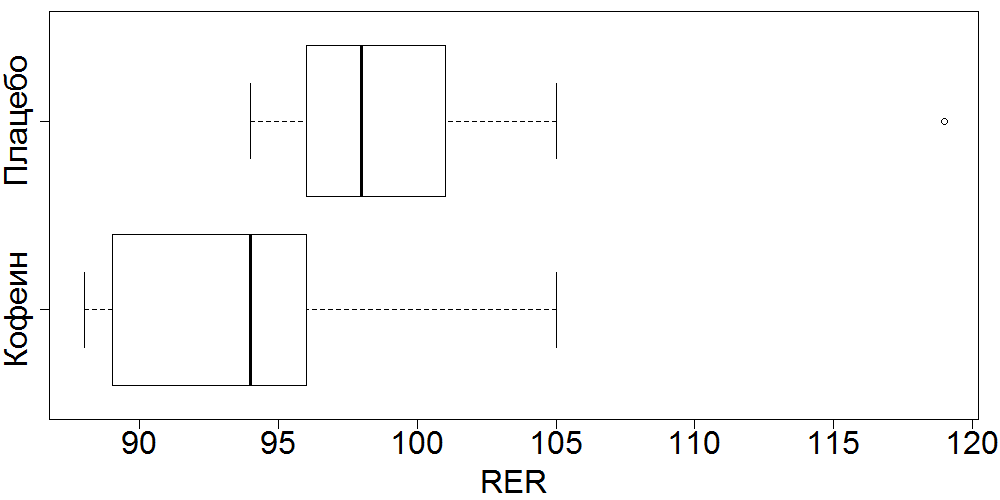
\includegraphics[width=0.4\textwidth]{rer.png}
	\end{figure}

Повлиял ли кофеин на значение RER?

 \bigskip
 $H_0\colon$ среднее значение показателя респираторного обмена не отличается в~двух группах.

 $H_1\colon$ среднее значение показателя респираторного обмена отличается в~двух группах.
 }

 \only<7>{
  \begin{center}
     \begin{tabular}{|c| c| c| c| c|} \hline
     Ранг & Наблюдение & Номер наблюдения & Наблюдение & Ранг\\ \hline
     16.5 & 105 & 1 & 96  & 9   \\
     18   & 119 & 2 & 99  & 13  \\
     14   & 100 & 3 & 94  & 5.5 \\
     11   & 97  & 4 & 89  & 3   \\
     9    & 96  & 5 & 96  & 9   \\
     15   & 101 & 6 & 93  & 4   \\
     5.5  & 94  & 7 & 88  & 1.5 \\
     7    & 95  & 8 & 105 & 16.5\\
     12   & 98  & 9 & 88  & 1.5 \\ \hline
     \end{tabular}
  \end{center}

  \bigskip

  Статистика $R_1$ "--- сумма рангов в одной из групп.

  \bigskip

  $p=0.0521,$ сдвиг между средними~--- $6$~пунктов, ($95$\% доверительный интервал~---  $\left[-0.00005, 12\right]$~пт).
 }
\end{frame}

\begin{frame}[label=siegel]{\hyperlink{classification}{\beamerbutton{(6)}} Критерий Ансари-Брэдли}
    \only<1>{\small
      \begin{center}
        \begin{tabular}{rl}
            выборки:                        & $X_1^{n_1}=\left(X_{11},\ldots,X_{1n_1}\right)$ \\
                                            & $X_2^{n_2}=\left(X_{21},\ldots,X_{2n_2}\right)$ \\
                                            & выборки независимые, $ \med(X_1) = \med(X_2) $ \\
%                                            &  \\
            нулевая гипотеза:               & $H_0\colon \mathbb{D} X_{1} = \mathbb{D} X_{2}$ \\
            альтернатива:                   & $H_1\colon \mathbb{D} X_{1} <\neq> \mathbb{D} X_{2}$ \\
            статистика:                     & $X_{(1)}\leq\ldots\leqslant  X_{(N)}$ --- вариационный ряд \\
                                            & объединённой выборки $X^N = X_1^{n_1} \bigcup X_2^{n_2}, N=n_1+n_2$ \\
                                            & $R_1\left(X_1^{n_1}, X_2^{n_2}\right) = \sum\limits_{i=1}^{n_1} \widetilde{\rank}\left(X_{1i}\right)$ \\
            нулевое распределение:          & табличное\\
            в Python:& \alert{\texttt{scipy.stats.ansari(x1, x2)}}
        \end{tabular}
        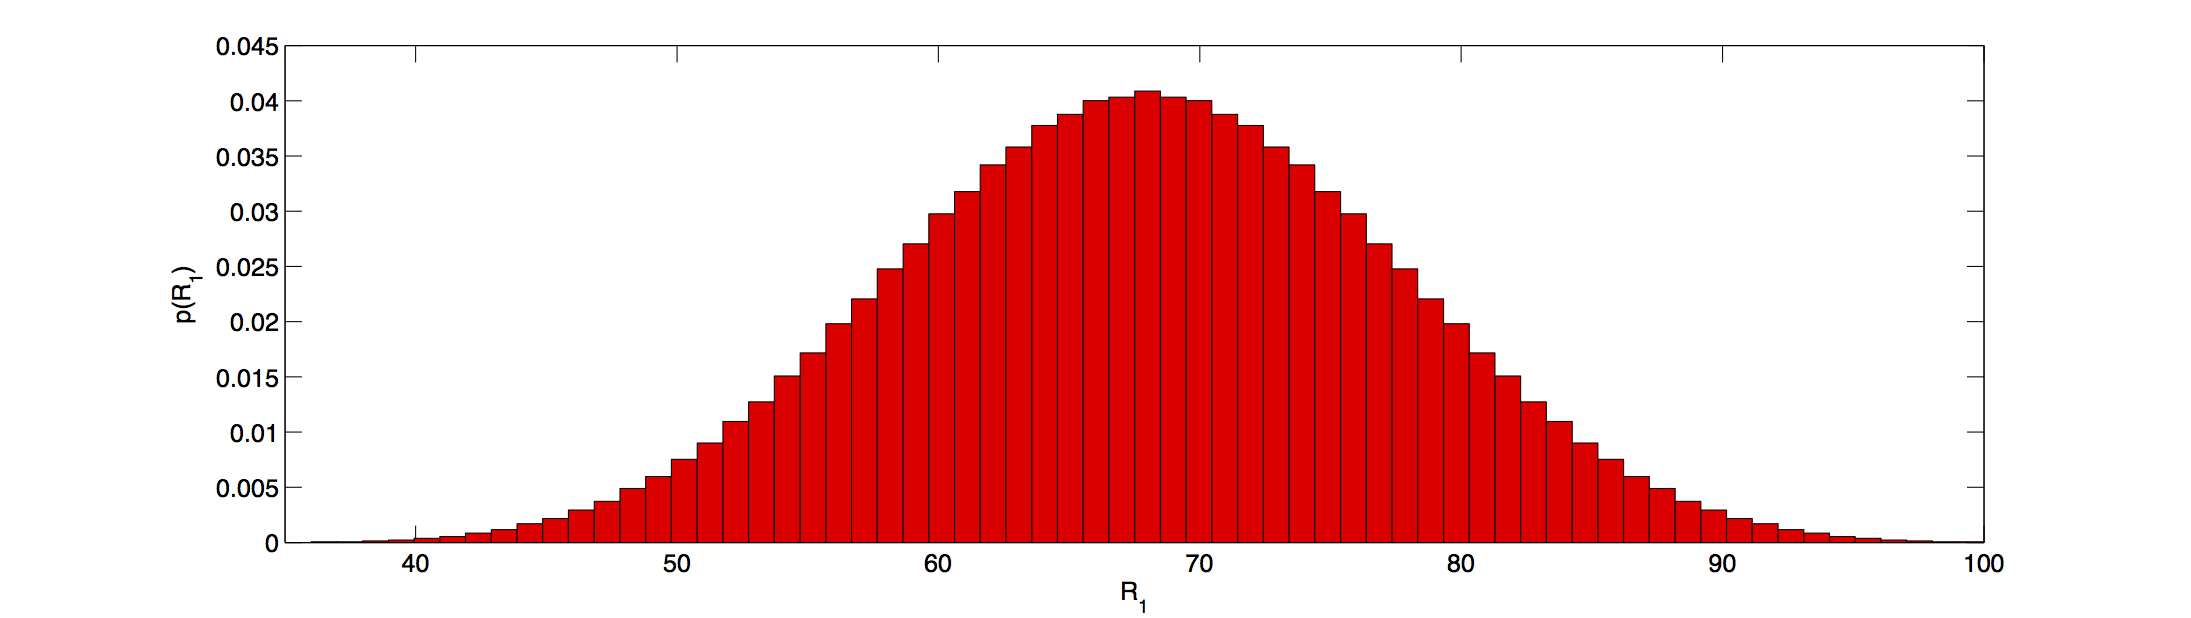
\includegraphics[width=0.8\textwidth]{mann.png}
    \end{center}
    }

    \only<2>{
     Ранги присваиваются от краёв к центру:
      \begin{center}\setlength{\tabcolsep}{2pt}
        \begin{tabular}{cccccccccccccc}
        $X_{(i)}$                       & $X_{(1)}$ &$\leq$& $X_{(2)}$ &$\leq$& $X_{(3)}$ &$\leq$& $\ldots$ &$\leq$ &$X_{(N-2)}$ &$\leq$& $X_{(N-1)}$ &$\leq$& $X_{(N)}$ \\
        $\widetilde{\rank}\left(X_{(i)}\right)$ & 1         &      &  2        &      & 3         &      &          &       & 3          &      &    2        &      & 1
        \end{tabular}
          \end{center}
    }

    \only<3>{
    \begin{block} {Пример,Bonnini, табл. 2.1} Два поставщика шестнадцатикилограммовых свинцовых слитков выслали по выборке образцов. Средний вес образцов в~обеих выборках соответствует норме; различаются ли дисперсий
    \end{block}
    \begin{figure}
    	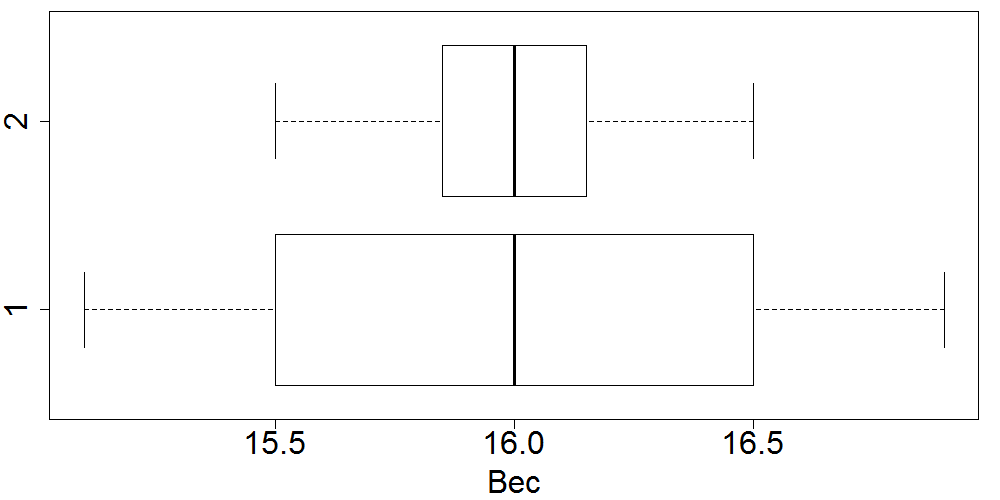
\includegraphics[width=0.4\textwidth]{ingots.png}
    \end{figure}

    \bigskip

    $H_0\colon$ дисперсия веса слитков не отличается для двух поставщиков.

    $H_1\colon$ дисперсия веса слитков для двух поставщиков отличается $ \Rightarrow p = 0.014$.
}
\end{frame}

\section{Перестановки}
\begin{frame}{Перестановочные критерии}
%%%%%%%%%%%%%%%%%%%%%%%%%%%%%%%%%%%%%%%%%%%%%%%%%%%%%%%%%%%%%%%%%%%%%%%
% При использовании ранговых критериев выборки превращают в ранги, затем делается какое-то дополнительное предположение, и на основании этого предположения получается, что разные конфигурации этих рангов при справедливости нулевой гипотезы могут реализоваться с равной вероятностью.
%Далее необходимо перебрать все конфигурации, и на каждой посчитать значение статистики — таким образом оценивается ее нулевое распределение.
% Если в этом алгоритме пропустить первый пункт (не превращать наблюдения в ранги), а остальное делать точно так же, то получится алгоритм работы перестановочных критериев.
%%%%%%%%%%%%%%%%%%%%%%%%%%%%%%%%%%%%%%%%%%%%%%%%%%%%%%%%%%%%%%%%%%%%%%%
	Ранговые критерии:
	\begin{enumerate}
		\item выборки $\Rightarrow$ ранги
        \bigskip
		\item дополнительное предположение (о равенстве распределений / медиан и пр.)
        \bigskip
		\item перестановки  $\Rightarrow$ нулевое распределение статистики
	\end{enumerate}

	\bigskip

	\textbf{Что если пропустить пункт 1?}
\end{frame}


\begin{frame}
\only<1>{
 \textbf{Пример} (зеркала в клетках мышей):

      $H_0\colon$ в клетке с зеркалом мыши проводят в среднем половину времени.

      $H_1\colon$ в клетке с зеркалом мыши проводят в среднем не половину времени.

      \bigskip

Проинтерпретируем задачу по-другому:

      $H_0\colon$ \textit{матожидание} времени в клетке с зералом равняется 0.5.

      $H_1\colon$ \textit{матожидание} времени в клетке с зералом не равняется 0.5

}
\only<2>{
\textbf{Предположение:}\\
время, проведенное мышами в клетке с зеркалом симметрично относительно матожидания.

Тогда при верности $H_0$: $X  - 0.5 $ --- симметрично относительно нуля.

\bigskip

\textbf{Статистика:}\\
$T=\sum\limits_{i=1}^n \left(X_i-0.5\right).$

\bigskip

\textbf{Как получить нулевое распределение:}\\
будем переставлять элементы  смещенной выборки $X  - 0.5 $ относительно нуля.
}
\only<3>{
 \textbf{Пример}:

      $H_0\colon$ в клетке с зеркалом мыши проводят в среднем половину времени.

      $H_1\colon$ в клетке с зеркалом мыши проводят в среднем не половину времени.

      \bigskip

     Статистика: $T=\sum\limits_{i=1}^n \left(X_i-0.5\right);\;\; t=-0.3784.$

     \bigskip

     \begin{center}
         \includegraphics[width=0.\textwidth]{perm_mouse-eps-converted-to.pdf}
     \end{center}

     \bigskip

     $p=\frac{\#\left[\left|T\right|\geq\left|t\right|\right]}{2^n} = 0.2292.$

     95\% доверительный интервал для доли времени в клетке с зеркалом (BCa бутстреп)~--- $\left[0.447,  0.511\right]$.
     }
\end{frame}

\subsection{Одна выборка}
\begin{frame}[label=perm1s]{\hyperlink{classification}{\beamerbutton{(8)}} Одновыборочный перестановочный критерий, гипотеза о~среднем}
%%%%%%%%%%%%%%%%%%%%%%%%%%%%%%%%%%%%%%%%%%%%%%%%%%%%%%%%%%%%%%%%%%%%%%%
% Имеется выборка размера n: и делается предположение, что функция распределения F (x) симметрична относительно математического ожидания. Одновыборочный перестановочный критерий проверяет нулевую гипотезу о значении математического ожидания случайной величины, из которой взята выборка.
% Если нулевая гипотеза этого критерия справедлива, каждый из объектов выборки мог с одинаковой вероятностью реализоваться слева и справа от математического ожидания. Поэтому нужно перебрать все 2n знаков, которые могут стоять в выражении для статистики перед разностью xi?m0. На основании этого перебора и будет восстановлено нулевое распределение статистики.
%%%%%%%%%%%%%%%%%%%%%%%%%%%%%%%%%%%%%%%%%%%%%%%%%%%%%%%%%%%%%%%%%%%%%%%
	\only<1>{
   \begin{center}
     \begin{tabular}{rl}
         выборка:                        & $X_1^n=\left(X_1,\ldots,X_n\right)$\\
					                     & $F\left(X\right)$ симметрично относительно матожидания\\
         нулевая гипотеза:               & $H_0\colon \mathbb{E}X = m_0$ \\
         альтернатива:                   & $H_1\colon \mathbb{E}X <\neq> m_0$ \\
         статистика:                     & $T\left(X^{n}\right) = \sum\limits_{i=1}^n \left(X_i-m_0\right)$ \\
		 нулевое распределение:          & порождается перебором $2^n$ знаков \\
		                                 & перед слагаемыми $X_i-m_0$\\
     \end{tabular}
 \end{center}

 \bigskip

 Достигаемый уровень значимости~--- доля перестановок знаков, на которых получилось такое же или ещё более экстремальное значение статистики.
 }

 \only<2>{
 \textbf{Пример} (диаметры шайб):

	Критерий знаковых рангов:
	\begin{center}
		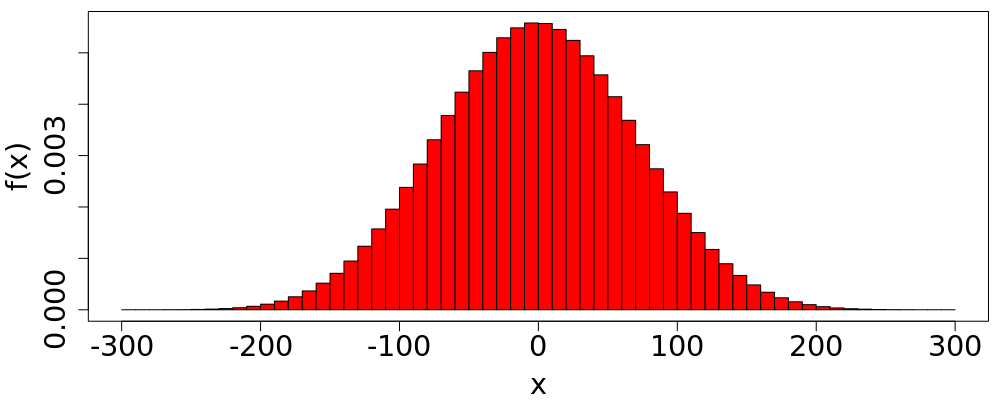
\includegraphics[width=0.35\textwidth]{ranksum24.png}
	\end{center}
	\vspace{-10pt}
	$p=0.0673$

	\bigskip

	Перестановочный критерий:
	\begin{center}
		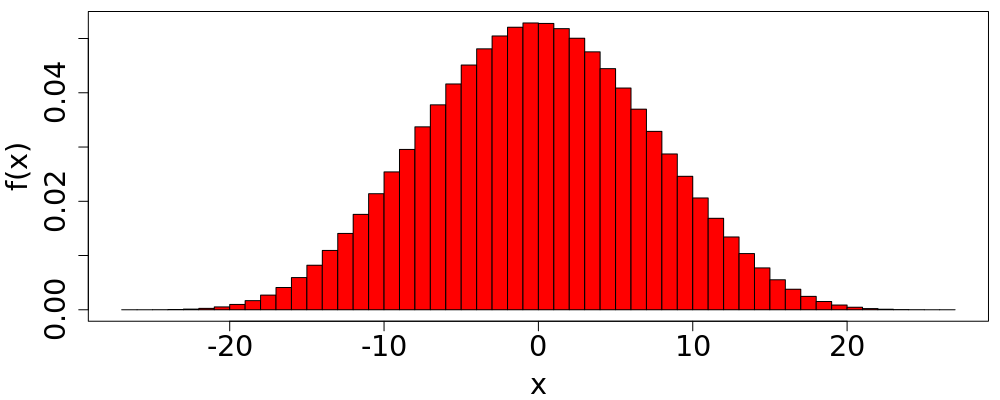
\includegraphics[width=0.35\textwidth]{perm_wash.png}
	\end{center}
	\vspace{-10pt}
	$T=14.6, p=0.1026$

     95\% доверительный интервал для среднего диаметра (BCa бутстреп)~--- $\left[10.11, 11.20\right]$.
 }
\end{frame}

\subsection{Две выборки}
\begin{frame}[label=perm2ss]{\hyperlink{classification}{\beamerbutton{(9)}} Двухвыборочный перестановочный критерий, гипотеза о средних, связанные выборки}
\only<1>{
   \begin{center}
     \begin{tabular}{rl}
         выборки:                        & $X_1^n=\left(X_{11},\ldots,X_{1n}\right)$\\
		     				             & $X_2^n=\left(X_{21},\ldots,X_{2n}\right)$ \\
								         & выборки связанные\\
								         & распределение попарных разностей симметрично\\
         нулевая гипотеза:               & $H_0\colon \mathbb{E}\left(X_1-X_2\right) = 0$ \\
         альтернатива:                   & $H_1\colon \mathbb{E}\left(X_1-X_2\right) <\neq> 0$ \\
         статистика:                     & $D_i = X_{1i}-X_{2i}$\\
                                         & $T\left(X_1^n, X_2^n\right)  = \sum\limits_{i=1}^n D_i$\\
		 нулевое распределение:          & порождается перебором $2^n$ знаков \\
										 & перед слагаемыми $D_i$\\
     \end{tabular}
 \end{center}
 }

 \only<2>{
     \textbf{Пример} (лечение депрессии):

	Критерий знаковых рангов:
	\begin{center}
		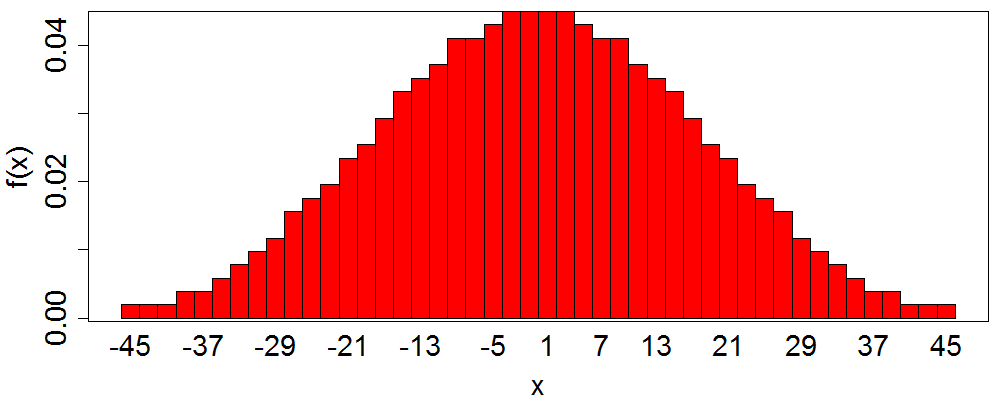
\includegraphics[width=0.35\textwidth]{ranksum9.png}
	\end{center}
	\vspace{-10pt}
	$p = 0.019$

	\bigskip

	Перестановочный критерий:
	\begin{center}
		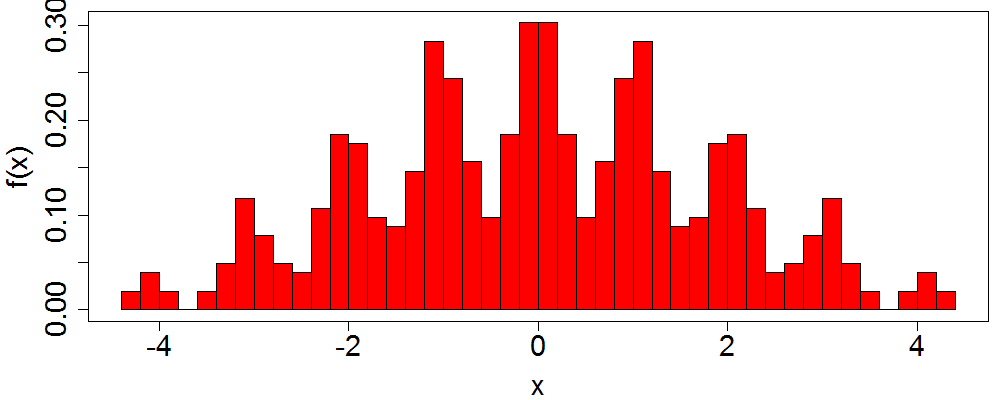
\includegraphics[width=0.35\textwidth]{perm_depr.png}
	\end{center}
	\vspace{-10pt}
	$T= 3.887, p=0.0137$

     95\% доверительный интервал для среднего уменьшения депрессивности (BCa бутстреп)~--- $\left[0.1658, 0.6834\right]$.
 }
\end{frame}

\begin{frame}[label=perm2sn]{\hyperlink{classification}{\beamerbutton{(10)}} Двухвыборочный перестановочный критерий, гипотеза о средних, независимые выборки}
\only<1>{
%%%%%%%%%%%%%%%%%%%%%%%%%%%%%%%%%%%%%%%%%%%%%%%%%%%%%%%%%%%%%%%%%%%%%%%
% Перестановочный критерий для независимых выборок выглядит абсолютно так же, как критерий Манна- Уитни за исключением того, что не производятся ранговые преобразования.
%%%%%%%%%%%%%%%%%%%%%%%%%%%%%%%%%%%%%%%%%%%%%%%%%%%%%%%%%%%%%%%%%%%%%%%
\begin{center}
\begin{tabular}{rl}
				выборки:                        & $X_1^{n_1}=\left(X_{11},\ldots,X_{1n_1}\right)$         \\
												& $X_2^{n_2} = \left(X_{21},\ldots,X_{2n_2}\right)$ \\
				нулевая гипотеза:               & $H_0\colon F_{X_1}\left(x\right) = F_{X_2}\left(x\right)$ \\
				альтернатива:                   & $H_1\colon F_{X_1}\left(x\right) = F_{X_2}\left(x+\Delta\right), \Delta <\neq> 0$ \\
				статистика:                     & $T\left(X_1^{n_1}, X_2^{n_2}\right) = \frac1{n_1}\sum\limits_{i=1}^{n_1} X_{1i} - \frac1{n_2}\sum\limits_{i=1}^{n_2} X_{2i}$ \\
				нулевое распределение:          & порождается перебором $C_{n_1+n_2}^{n_1}$ \\
												& размещений объединённой выборки\\
			\end{tabular}
 \end{center}
 }
 \only<2>{
     \textbf{Пример} (кофеин и респираторный обмен):

	Критерий Манна-Уитни:
	\begin{center}
		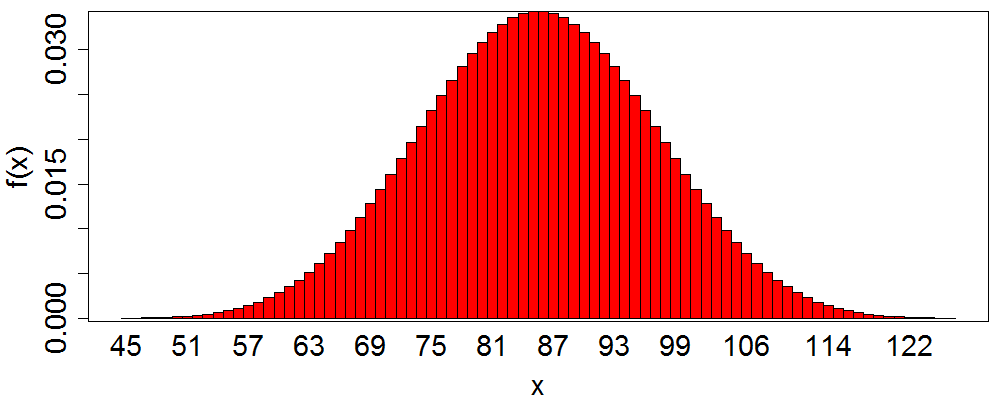
\includegraphics[width=0.35\textwidth]{MU9-9.png}
	\end{center}
	\vspace{-10pt}
	$p=0.0521$

	\bigskip

	Перестановочный критерий:
	\begin{center}
		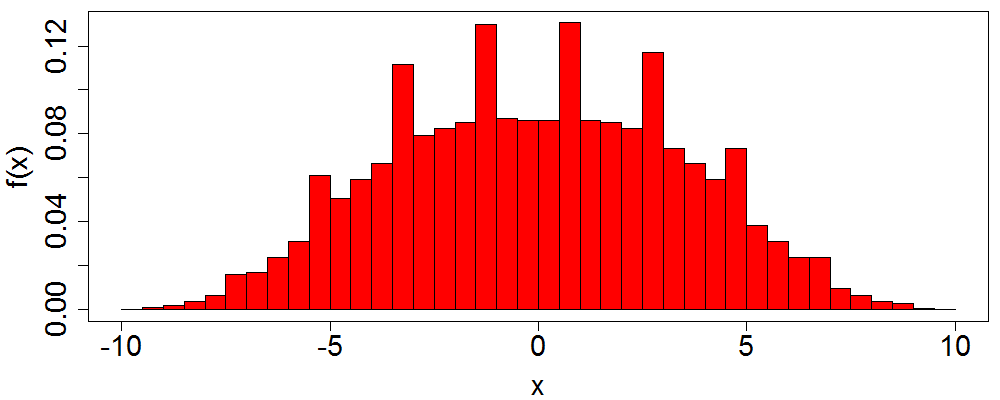
\includegraphics[width=0.35\textwidth]{perm_rer.png}
	\end{center}
	\vspace{-10pt}
	$T= 6.33, p=0.0578$

	 95\% доверительный интервал для разности средних (BCa бутстреп)~--- $\left[1.556, 13.667\right]$.
 }
\end{frame}
%%%%%%%%%%%%%%%%%%%%%%%%%%%%%%%%%%%%%%%%%%%%%%%%%%%%%%%%%%%%%%%%%%%%%%%
%Good:  3.7.2.
% Не самый мощный критерий, поскольку (интуитивно) нам пришлось пожертвовать двумя наблюдениями, чтобы перейти к попарными разностям. Аналог этого критерия
%%%%%%%%%%%%%%%%%%%%%%%%%%%%%%%%%%%%%%%%%%%%%%%%%%%%%%%%%%%%%%%%%%%%%%%
\begin{frame}[label=perm2d]
\frametitle{\hyperlink{classification}{\beamerbutton{(11)}} Двухвыборочный перестановочный критерий, гипотеза о~дисперсиях, статистика Али}

	\only<1>{
   \begin{center}
     \begin{tabular}{rl}
         выборки:                        & $X_1^{n}=\left(X_{11},\ldots,X_{1n}\right)$\\
                                         & $X_2^{n}=\left(X_{21},\ldots,X_{2n}\right)$ \\
                                         & выборки независимые\\
         нулевая гипотеза:               & $H_0\colon \mathbb{D} X_{1} = \mathbb{D} X_{2}$ \\
         альтернатива:                   & $H_1\colon \mathbb{D} X_{1} <\neq> \mathbb{D} X_{2}$ \\
         статистика:                     &  $\delta\left(D_1^{n-1}\right) = \sum\limits_{i=1}^{n-1} i(n-i)D_{1i},$ \\
					                     & $D_{1i} = X_{1(i+1)} - X_{1(i)}$\\
		нулевое распределение:           & порождается перебором $2^{n-1}$ \\
										 & попарных перестановок $D_{1i}$ и~$D_{2i}$\\
     \end{tabular}
 \end{center}
 }
\end{frame}

\begin{frame}{Особенности перестановочных критериев}
%%%%%%%%%%%%%%%%%%%%%%%%%%%%%%%%%%%%%%%%%%%%%%%%%%%%%%%%%%%%%%%%%%%%%%%
% У перестановочных критериев есть некоторые особенности, о которых очень важно помнить.
% Статистику для перестановочных критериев можно выбирать по-разному. В некоторых случаях это приводит к одному и тому же достигаемому уровню значимости, то есть ни на что не влияет. Например, в одновыборочной задаче, проверяя гипотезу о равенстве нулю математического ожидания в качестве статистики перестановочного критерия можно использовать как сумму элементов выборки, так и выборочное среднее. Нулевые распределения этих статистик будут отличаться только сдвигом и масштабом, поэтому достигаемый уровень значимости, посчитанный по ним, будет одним и тем же.
% В других случаях, по-разному выбирая статистику для перестановочного критерия, можно получать разные достигаемые уровни значимости. Например, для статистик ... и ... нулевые распределения отличаются не только сдвигом и масштабом, поэтому достигаемый уровень значимости у критериев с этими двумя вариантами статистик тоже будет разный. Поэтому при выборе статистики для перестановочного критерия важно думать о том, какие из свойств исходной случайной величины для наиболее важны.
% Перестановочные критерии придумал Рональд Фишер еще в начале XX века, однако их начали активно использовать только с появлением и широким распространением компьютеров, потому что для вычисле- ния нулевых распределений этих критериев используются перестановки. В отличие от ранговых критериев, нормальных аппроксимаций для нулевого распределения в случае больших выборок не существует, поэтому единственный способ оценить нулевое распределение статистики — это перебрать много перестановок. По- этому точно посчитать достигаемый уровень значимости перестановочного критерия на больших выборках достаточно сложно. Однако его можно посчитать приближённо. Для этого нужно взять какое-то случайное подмножество G? множества всех возможных перестановок G. При этом стандартное отклонение достигаемого уровня значимости будет примерно равно   .... На практике, чтобы получить хорошую аппроксимацию достигаемого уровня значимости, достаточно взять несколько тысяч перестановок.
%%%%%%%%%%%%%%%%%%%%%%%%%%%%%%%%%%%%%%%%%%%%%%%%%%%%%%%%%%%%%%%%%%%%%%%
 \begin{itemize}
 \item Статистику критерия можно выбрать разными способами. В~некоторых случаях разные статистики приведут к одному и тому же достигаемому уровню значимости:
 $$X^n, \;\; H_0\colon \mathbb{E}X = 0, \; H_1\colon \mathbb{E}X \neq 0,$$
 $$T_1\left(X^n\right) = \sum\limits_{i=1}^n X_i \;\;\sim \;\; T_2\left(X^n\right) = \bar{X}.$$
 В других случаях достигаемый уровень значимости будет зависеть от выбора статистики:
 $$T_2\left(X^n\right) = \bar{X} \;\; \nsim \;\; T_3\left(X^n\right) = \frac{\bar{X}}{S/\sqrt{n}}.$$
 \item Если множество перестановок $G$ слишком велико, для оценки нулевого распределения $T$ достаточно взять случайное подмножество $G'\in G.$ При этом стандартное отклонение достигаемого уровня значимости будет равно примерно $\sqrt{\frac{p\left(1-p\right)}{\left|G'\right|}}.$
 \end{itemize}
\end{frame}

\subsection{Бутстреп}
\begin{frame}{Перестановки и бутстреп}
%%%%%%%%%%%%%%%%%%%%%%%%%%%%%%%%%%%%%%%%%%%%%%%%%%%%%%%%%%%%%%%%%%%%%%%
% Доверительные интервалы для параметров тесно связаны с проверкой точечных гипотез об их значениях. Например, z-критерии для средних связаны с нормальными доверительными интервалами, критерии Стьюдента соответствуют доверительным интервалам, построенным с использованием распределения Стьюдента. Для перестановочных критериев ближайшим аналогом в мире доверительных интервалов является метод бутстрепа, однако отношения между ними не такие взаимнооднозначные.
% Перестановочные критерии принимают на вход выборку (или выборки), считают на них какую-то статистику. Далее делается дополнительное предположение о распределении, из которого эти выборки взяты. Это пред- положение порождает множество перестановок исходных данных, которые могли реализоваться с одинаковой вероятностью, если нулевая гипотеза справедлива. На этих перестановках вычисляется значение статистики и таким образом оценивается ее нулевое распределение.
% Бутстреп-методы работают в каком-то смысле похоже. На вход они также принимают выборку или выбор- ки и считают значение статистики, которая оценивает интересующий параметр. Далее на основании исходных данных генерируется множество бутстреп-псевдовыборок, и на этих псевдовыборках вычисляются значения интересующей статистики, то есть оценивается ее распределение.
% Ключевых различий между этими методами несколько. Во-первых, перестановочный критерий использует дополнительное предположение, которое позволяет породить множество перестановок, которые используются для построения распределения. Во-вторых, перестановки, используемые в перестановочном критерии, — это выборки без возвращения, в то время как бутстреп-методы используют выборки с возвращением (бутстреп- псевдовыборки могут содержать по несколько копий элементов исходной выборки). Кроме того, распреде- ления, которые получаются при использовании этих методов, абсолютно разные, потому что распределение статистики перестановочного критерия — это то распределение, которое статистика будет иметь при спра- ведливости нулевой гипотезы, в то время как распределение бутстреп-статистики не подразумевает никакой нулевой гипотезы.
%%%%%%%%%%%%%%%%%%%%%%%%%%%%%%%%%%%%%%%%%%%%%%%%%%%%%%%%%%%%%%%%%%%%%%%
	Перестановочные критерии:
	\begin{enumerate}
		\item выборки, статистика
		\item дополнительное предположение
		\item перестановки  $\Rightarrow$ нулевое распределение статистики
	\end{enumerate}

	\bigskip

	Бутстреповые доверительные интервалы:
	\begin{enumerate}
		\item выборки, статистика, оценивающая параметр
		\item бутстреп-псевдовыборки  $\Rightarrow$ приближённое распределение статистики
	\end{enumerate}
\end{frame}

\begin{frame}
%%%%%%%%%%%%%%%%%%%%%%%%%%%%%%%%%%%%%%%%%%%%%%%%%%%%%%%%%%%%%%%%%%%%%%%
% Давайте считать, что мы находимся в реальном мире и доступа к генеральной совокупности у нас нет, а есть только  выборка объёма n. Давайте из этой выборки сделаем много псевдовыборок - выборок с возвращениями - того же самого объёма n. На каждой псевдовыборке посчитаем значение статистики; оказывается, что распределение значений статистики на псевдовыборках часто является хорошей оценкой истинного распределения статистики. Так работает бутстреп (слово означает петлю, которая пришита к заднему краю армейских ботинок, и отсылает нас к выражению "to pull oneself up by one's bootstraps" - что-то вроде Мюнхаузена, вытаскивающего себя из болота за волосы. Действительно, это выглядит как магия.
%%%%%%%%%%%%%%%%%%%%%%%%%%%%%%%%%%%%%%%%%%%%%%%%%%%%%%%%%%%%%%%%%%%%%%%
		\begin{itemize}
			\item бутстреп:
		\end{itemize}
		\begin{figure}
			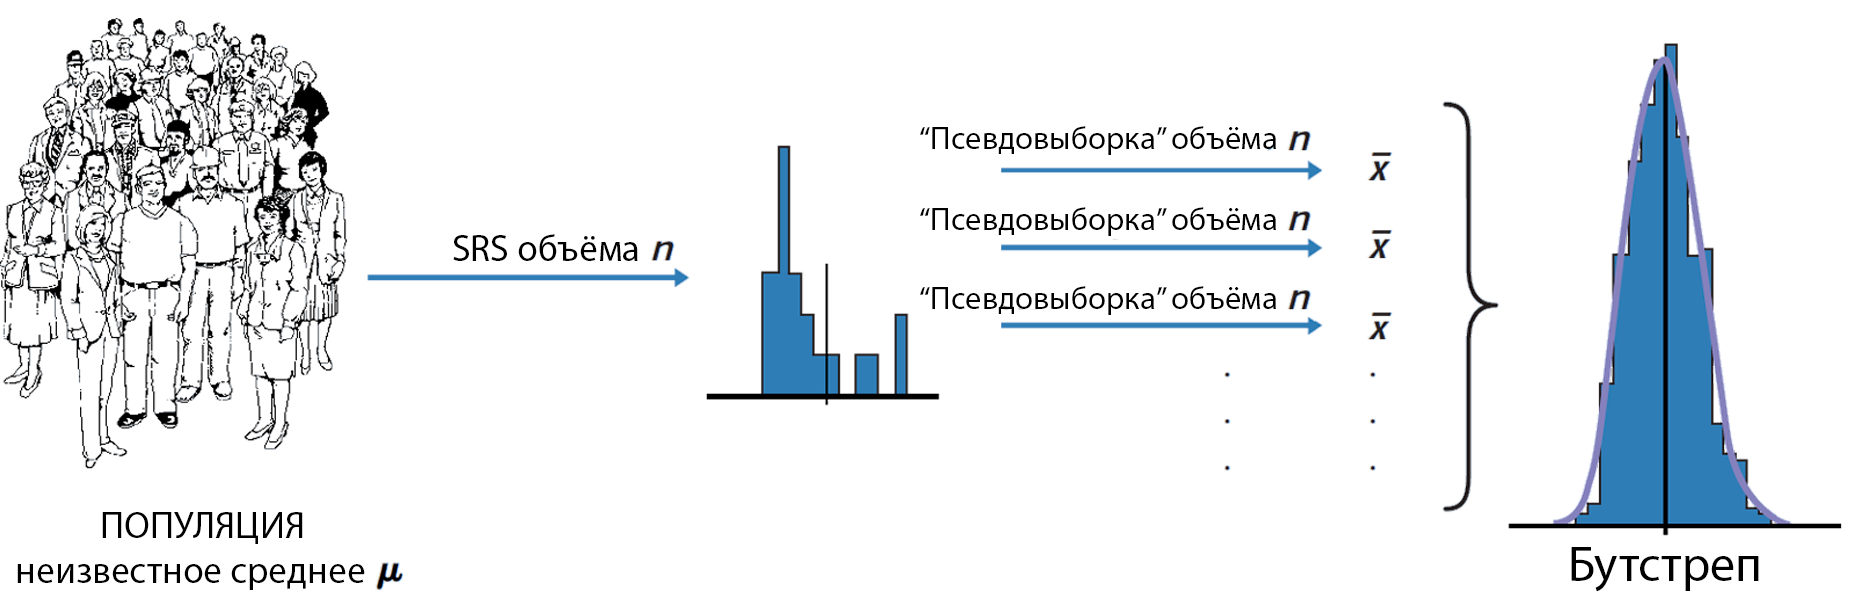
\includegraphics[width=0.8\textwidth]{boot3.png}
		\end{figure}
		Сгенерировать $N$ <<псевдовыборок>> объёма $n$ и оценить выборочное распределение $\hat{\theta}_n$ <<псевдоэмпирическим>>.

\end{frame}


\begin{frame}{Кофеин и респираторный обмен}
	\only<1>{
%%%%%%%%%%%%%%%%%%%%%%%%%%%%%%%%%%%%%%%%%%%%%%%%%%%%%%%%%%%%%%%%%%%%%%%
% Чтобы лучше это понять, можно вспомнить пример с кофеином и респираторным обменом. В этой задаче проверялась гипотеза H0 : среднее значение показателя респираторного обмена не отличается в двух группах. Эта нулевая гипотеза проверялась против односторонней альтернативы H1 : под воздействием кофеина среднее значение показателя респираторного обмена снижается.
% На рисунке 6.16 показано нулевое распределение перестановочного критерия со статистикой X ?1n ? X ?2n. На рисунке 6.17 — бутстреп-распределение той же самой статистики X ?1n ? X ?2n. Ключевое различие между этими двумя распределениями в том, что они центрированы в разных местах. Перестановочное нулевое рас- пределение центрировано в нуле — значении, соответствующем нулевой гипотезе. Бутстреп-распределение, в свою очередь, центрировано в выборочном среднем значений параметра. Параметр в данном случае — это разность средних, то есть центр бутстреп-распределения — это 6.33.
% Для перестановочного критерия доля перестановок, на которых среднее больше либо равно 6.33 (выборочное среднее, которое реализовано в данных) составляет примерно 0.03 (рисунок 6.18). Это и есть достигаемый уровень значимости перестановочного критерия, и он точный.
% На бутстреп-распределении той же самой статистки доля псевдовыборок, на которых среднее меньше либо равно нулю, составляет 0.011 (рисунок 6.19). Эту величину можно считать приближенным достигаемым уровнем значимости бутстреп-критерия. То есть с помощью доверительных интервалов на основе бутстрепа тоже можно проверять гипотезы, однако нужно это делать немного иначе.
%%%%%%%%%%%%%%%%%%%%%%%%%%%%%%%%%%%%%%%%%%%%%%%%%%%%%%%%%%%%%%%%%%%%%%%
	\begin{figure}
		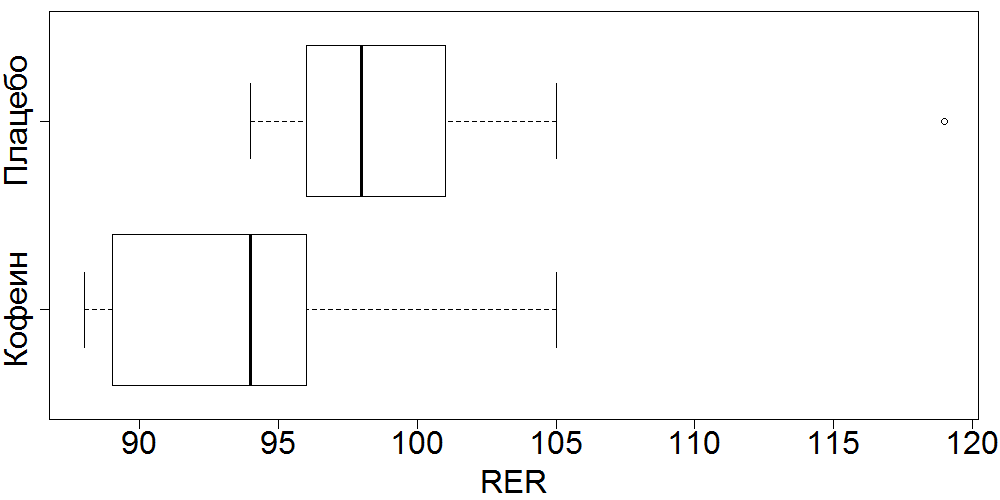
\includegraphics[width=0.5\textwidth]{rer.png}
	\end{figure}
	$H_0\colon$ среднее значение показателя респираторного обмена не отличается в~двух группах.

	$H_1\colon$ под воздействием кофеина среднее значение показателя респираторного обмена снижается.

	$\bar{X}_{1n} - \bar{X}_{2n} = 6.33$
}
\only<2>{
	Нулевое распределение перестановочного критерия со~статистикой $\bar{X}_{1n} - \bar{X}_{2n}$:
	\begin{center}
		\includegraphics[width=0.5\textwidth]{rer_perm.png}
	\end{center}

	\bigskip

	Бутстреп-распределение статистики $\bar{X}_{1n} - \bar{X}_{2n}$:
	\begin{center}
		\includegraphics[width=0.5\textwidth]{rer_meanchange_boot.png}
	\end{center}
}
\only<3>{
	Нулевое распределение перестановочного критерия со~статистикой $\bar{X}_{1n} - \bar{X}_{2n}$:
	\begin{center}
		\includegraphics[width=0.8\textwidth]{rer_perm'.png}
	\end{center}

	Доля перестановок, на которых среднее больше либо равно $6.33$~--- $0.0289$.

	Это точный достигаемый уровень значимости перестановочного критерия.
}
\only<4>{
	Бутстреп-распределение статистики $\bar{X}_{1n} - \bar{X}_{2n}$:
	\begin{center}
		\includegraphics[width=0.8\textwidth]{rer_meanchange_boot'.png}
	\end{center}

	Доля псевдовыборок, на которых среднее меньше либо равно нулю~--- $0.011$.

	Это приближённый достигаемый уровень значимости бутстреп-критерия.
}
\end{frame}

\begin{frame}{Перестановки vs. бутстреп}
%%%%%%%%%%%%%%%%%%%%%%%%%%%%%%%%%%%%%%%%%%%%%%%%%%%%%%%%%%%%%%%%%%%%%%%
% Перестановочный критерий с помощью нулевого распределения статистики измеряет расстояние от 0 до D ?n — значения параметра, реализовавшегося в эксперименте. Бутстреп-критерий измеряет, наоборот, расстояние от D ?n до 0.
% Перестановочный критерий является более точным, потому что в нем перебирается подмножество всех возможных перестановок данных, которые равновероятны при справедливости нулевой гипотезы. Бутстреп- критерий в описанном выше виде является только приближенным, поскольку в нем всегда перебирается только конечное подмножество всех возможных бутстреп-псевдовыборок, потому что их заведомо слишком много.
% Самое важное различие между этими двумя критериями заключается в том, что они проверяют разные ги- потезы, поскольку перестановочный критерий использует дополнительные предположения. Перестановочный критерий проверяет гипотезу полного равенства распределений в двух выборках и проверяется она против альтернативы сдвига (в этом примере односторонней). Предполагается, что никак иначе, кроме как сдвигом, эти распределения отличаться не могут.
% Бутстреп-критерий проверяет всего лишь гипотезу о равенстве математических ожиданий: Гипотезу равенства он проверяет против односторонней альтернативы точно так же, как и перестановочный критерий. Однако эта гипотеза заведомо более общая: не используется предположение равенстве функций распределения в двух выборках.
% Проверка гипотез с помощью бутстрепа — это достаточно сложная задача. Показанный небольшой двухвыборочный пример позволяет понять плюсы и минусы бутстрепа и перестановочных критериев.
% Бутстреп тоже позволяет проверять гипотезы, причём гораздо более широкого класса. Поскольку этот метод не использует дополнительных предположений, можно проверять только интересующий параметр (в примере это была разность математических ожиданий). Кроме того, с помощью бутстрепа можно проверять и другие крайне экзотические гипотезы, которые никакими другими методами проверить нельзя. Например, гипотеза о том, что распределение имеет ровно две моды.
% Если предположения, лежащие в основе перестановочного критерия, выполняются, то перестановочный критерий, во-первых, точнее, поскольку его достигаемый уровень значимости точный, во-вторых, всегда мощнее, чем аналогичный критерий бутстрепа. Но бутстреп при этом гораздо более гибок, потому что его можно использовать в ситуациях, когда не выполняются предположения, использующиеся в перестановочном критерии.
%%%%%%%%%%%%%%%%%%%%%%%%%%%%%%%%%%%%%%%%%%%%%%%%%%%%%%%%%%%%%%%%%%%%%%%
    \centering
    \begin{tabular}{|c|c|}
    \hline
    \bf Перестановочный критерий & \bf Бутстреп-критерий\\
    \hline
    Центр в нуле & Центр в точечной оценке \\ \hline
    Точный & Приближенный \\ \hline
    $H_0\colon F_{X_1}(x) = F_{X_2}(x)$ & $H_0\colon \mathbb{E}X_1 = \mathbb{E}X_2$ \\
    $H_1\colon F_{X_1}(x) = F_{X_2}(x+\Delta), \Delta>0$ & $H_1\colon \mathbb{E}X_1 > \mathbb{E}X_2$\\\hline
    \end{tabular}

\end{frame}



\section{Распределения}

\begin{frame}{Различия между моментами высокого порядка}
 \begin{center}
     \includegraphics[width=0.8\textwidth,trim=30mm 0mm 30mm 5mm,clip]{distrdiff_example.png}
 \end{center}

 $X_1\sim \chi^2_4, \;\; X_2\sim N\left(4,\sqrt{8}\right);$

 $\mathbb{E}X_1=\mathbb{E}X_2, \;\; \mathbb{D}X_1 = \mathbb{D}X_2.$
\end{frame}

\subsection{Критерии согласия}
%%%%%%%%%%%%%%%%%%%%%%%%%%%%%%%%%%%%%%%%%%%%%%%%%%%%%%%%%%%%%%%%%%%%%%%
% первые два момента распределения - это еще не все распределение.
% Поэтому при проверке равенства распределений нужно пользоваться другими методами
% Kolmogorov-Smirnov has more power against deviations in the middle, with Cramer-von Mises in between the two (KS and Andersen-Darling) but somewhat more akin to the Kolmogorov-Smirnov in that respect (compared with Anderson-Darling which is missing on the slide)
% Тяжелые хвосты - используетйе АД https://www.researchgate.net/publication/267205556_Power_Comparisons_of_Shapiro-Wilk_Kolmogorov-Smirnov_Lilliefors_and_Anderson-Darling_Tests
%%%%%%%%%%%%%%%%%%%%%%%%%%%%%%%%%%%%%%%%%%%%%%%%%%%%%%%%%%%%%%%%%%%%%%%
\begin{frame}{Двухвыборочные критерии согласия}
   \begin{center}
     \begin{tabular}{rl}
         выборки:                        & $X_1^{n_1}=\left(X_{11},\ldots,X_{1n_1}\right)$ \\
                                         & $X_2^{n_2}=\left(X_{21},\ldots,X_{2n_2}\right)$ \\
                                         & выборки независимые \\
         нулевая гипотеза:               & $H_0\colon F_{X_1} \left(x\right) = F_{X_2} \left(x\right)$ \\
         альтернатива:                   & $H_1\colon H_0$ неверна \bigskip \\
         \multicolumn{2}{l}{\textbf{Критерий Смирнова}}\\
         статистика:                        & $D\left(X_1^{n_1}, X_2^{n_2}\right) = \sup\limits_{-\infty<x<\infty} \left|F_{n_1X_1} \left(x\right) - F_{n_2 X_2} \left(x\right)\right|$  \bigskip \\
         \multicolumn{2}{l}{\textbf{Критерий Андерсона} (модификация критерия Смирнова-Крамера-}\\
         \multicolumn{2}{l}{фон Мизеса)}\\
         статистика:                        & $T\left(X_1^{n_1}, X_2^{n_2}\right) = \frac1{n_1n_2\left(n_1+n_2\right)} \Biggl( n_1\sum\limits_{i=1}^{n_1} \left(\rank\left(X_{1i}\right) - i\right)^2 + $\\
                                            & \;\;\; $ + n_2 \sum\limits_{j=1}^{n_1} \left(\rank\left(X_{2j}\right) - j\right)^2 \Biggr) - \frac{4n_1n_2-1}{6\left(n_1+n_2\right)}$
     \end{tabular}
 \end{center}

 \bigskip

 Статистики имеют табличные распределения при $H_0$.
\end{frame}

%\subsection{Анализ выживаемости}


\section{}

\section{}
\begin{frame}[allowframebreaks]{Где что искать?}
   \begin{enumerate}
        \item Критерии нормальности:
        \begin{itemize}
            \item Харке-Бера (Jarque–Bera)~--- Кобзарь, 3.2.2.16
            \item Шапиро-Уилка (Shapiro-Wilk)~--- Кобзарь, 3.2.2.1
            \item хи-квадрат (chi-square)~--- Кобзарь, 3.1.1.1, 3.2.1.1
            \item согласия (goodness-of-fit), основанные на эмпирической функции распределения ~--- Кобзарь, 3.1.2, 3.2.1.2
        \end{itemize}

        \item Параметрические критерии для нормальных распределений:
        \begin{itemize}
            \item Z-критерии (Z-tests)~--- Kanji, №№ 1, 2, 3
            \item t-критерии Стьюдента (t-tests)~--- Kanji, №№ 7, 8, 9
            \item критерий хи-квадрат (chi-square test)~--- Kanji, №15
            \item критерий Фишера (F-test)~--- Kanji, №16
        \end{itemize}

        \item Критерии, основанные на правдоподобии: Bilder, раздел B.5

        \item Критерии для распределения Бернулли:
        \begin{itemize}
            \item всё про одновыборочную задачу~--- Agresti, 1.3, 1.4
            \item Z-критерии (Z-tests)~--- Kanji, №№ 4, 5
            \item точный критерий (exact binomial test)~--- McDonald, \url{http://www.biostathandbook.com/exactgof.html}
            \item доверительные интервалы Уилсона (score confidence intervals)~--- Newcombe, 1998a, 1998b, 1998c
        \end{itemize}

        \item непараметрические критерии:
        \begin{itemize}
            \item критерии знаков (sign tests)~--- Kanji, №№ 45, 46;
            \item критерии знаковых рангов (signed-rank tests)~--- Kanji, №№ 47, 48;
            \item критерий Манна-Уитни-Уилкоксона (Mann-Whitney-Wilcoxon test)~--- Kanji, № 52;
            \item перестановочные критерии (permutation tests)~--- Good, 3.2.1, 3.6.4, 3.7.2 (с ошибкой, исправлено в Ramsey);
            \item двухвыборочные критерии согласия (two-sample goodness-of-fit tests)~--- Кобзарь, 3.1.2.8.
        \end{itemize}
      \end{enumerate}

    \end{frame}
    \begin{frame}[allowframebreaks]{Литература}
        \begin{itemize}
            \item \href{https://stats.idre.ucla.edu/other/mult-pkg/faq/general/faqhow-are-the-likelihood-ratio-wald-and-lagrange-multiplier-score-tests-different-andor-similar/}{О сравнении ассимптотических критериев}
            \item Кобзарь А.И. \textit{Прикладная математическая статистика}, 2006.
            \item Королёв В.Ю. \textit{Теория вероятностей и математическая статистика}, 2008.

            \bigskip


\item Dinse G.E. (1982). \textit{Nonparametric estimation for partially-complete time and	type of failure data}. Biometrics, 38, 417–431.
\item Ramsey P.H., Ramsey P.P. (2008). \textit{Brief investigation of tests of variability in the two-sample case}. Journal of Statistical Computation and Simulation, 78(12), 1125--1131.
\item Bonnini S., Corain L., Marozzi M., Salmaso S. \textit{Nonparametric Hypothesis Testing - Rank and Permutation Methods with Applications in R}, 2014.
\item  Kanji G.K. \textit{100 statistical tests}, 2006.
\item Agresti A. \textit{Categorical Data Analysis}, 2013.
\item Bilder C.R., Loughin T.M. \textit{Analysis of Categorical Data with R}, 2013.
\item McDonald J.H. \textit{Handbook of Biological Statistics}, 2008.
\item Newcombe R.G. (1998). \textit{Improved confidence intervals for the difference between binomial proportions based on paired data}. Statistics in Medicine, 17, 2635–2650.
\item Newcombe R.G. (1998). \textit{Interval estimation for the difference between independent proportions: comparison of eleven methods}. Statistics in Medicine, 17, 873–890.
\item Newcombe R.G. (1998). \textit{Two-sided confidence intervals for the single proportion: comparison of seven methods}. Statistics in Medicine, 17, 857–872.
\item  NIST/SEMATECH. \textit{e-Handbook of Statistical Methods}. \url{http://www.itl.nist.gov/div898/handbook/}
\item  Efron B., Tibshirani R. \textit{An Introduction to the Bootstrap}, 1993.
\item Good P. \textit{Permutation, Parametric and Bootstrap Tests of Hypotheses: A Practical Guide to Resampling Methods for Testing Hypotheses}, 2005.
\item Hollander M., Wolfe D.A. \textit{Nonparametric statistical methods}, 1973.
\item Kanji G.K. \textit{100 statistical tests}, 2006.
\item Laureysens I., Blust R., De Temmerman L., Lemmens C., Ceulemans R. (2004). \textit{Clonal variation in heavy metal accumulation and biomass production in a poplar coppice culture. I. Seasonal variation in leaf, wood and bark concentrations.} Environmental Pollution, 131, 485-494.
\item Shekin D. \textit{Handbook of Parametric and Nonparametric Statistical Procedures}, 2007.
\item Shervin C.M. (2004) \textit{Mirrors as potential environmental enrichment for individually housed laboratory mice}. Applied Animal Behaviour Science, 87(1-2), 95--103.

\end{itemize}
\end{frame}


\end{document}

\begin{frame}{}{}
    \centering
    \bfseries
    \huge Множественные гипотезы
\end{frame}
\begin{frame}{Поиск экстрасенсов}
    \only<1>{
%%%%%%%%%%%%%%%%%%%%%%%%%%%%%%%%%%%%%%%%%%%%%%%%%%%%%%%%%%%%%%%%%%%%%%%
% Пример связан с исследованиями Джозефа Райна. Это американский ученый 50-х годов, который занимался исследованиями возможностей экстрасенсорного восприятия. Первый этап таких исследований — это поиск экстрасенсов. Джозеф Райн придумал для этого следующий эксперимент. Испытуемому предлагалось угадать цвета десяти карт, лежащих рубашкой вверх.
% Проверялась нулевая гипотеза H0 : испытуемый выбирает ответ наугад. Альтернативная гипотеза H1 : испытуемый может предсказывать цвета карт. Статистика t — число карт, цвета которых угаданы, — при справедливости нулевой гипотезы имеет биномиальное распределение с параметрами n = 10, p = 0.5, поскольку цвета только два, и они называются наугад. Вероятность правильно назвать цвета 9 и более карт равна примерно 0.01, то есть, если испытуемый угадывает 9 карт, получается достигаемый уровень значимости p примерно 0.01, и нулевую гипотезу можно с чистой совестью отклонить в пользу односторонней альтернативы.
%%%%%%%%%%%%%%%%%%%%%%%%%%%%%%%%%%%%%%%%%%%%%%%%%%%%%%%%%%%%%%%%%%%%%%%
        (Rhine, 1950): исследования возможности экстрасенсорного восприятия. Первый этап~--- поиск экстрасенсов.

        Испытуемому предлагается угадать цвет 10~карт.

        \bigskip

        \begin{center}
            \includegraphics[width=0.7\textwidth]{cards.png}
        \end{center}

        \bigskip

        $H_0\colon$ испытуемый выбирает ответ наугад.

        $H_1\colon$ испытуемый может предсказывать цвета карт.

        Статистика $t$~--- число карт, цвета которых угаданы.

        $$P\left(t\geq9\left|H_0\right.\right)=11\cdot\frac1{2}^{10} = 0.0107421875,$$
        т.\,е. при $t=9$ получаем достигаемый уровень значимости $p \approx 0.01$~--- можно отклонять $H_0$.
    }

    \only<2>{
%%%%%%%%%%%%%%%%%%%%%%%%%%%%%%%%%%%%%%%%%%%%%%%%%%%%%%%%%%%%%%%%%%%%%%%
% В экспериментах Джозефа Райна процедуру отбора прошли 1000 человек. Девять из них угадали цвета 9 из 10 карт, еще двое угадали все 10 карт. Ни один из этих испытуемых в последующих экспериментах не подтвердил своих способностей, из чего Джозеф Райн сделал вывод, что экстрасенсам нельзя говорить о том, что они экстрасенсы, потому что от этого их способности сразу пропадают. Однако очевидно, что проблема кроется в чем-то другом.
% Если принять гипотезу о том, что экстрасенсов не существует, то вероятность того, что из тысячи человек хотя бы один случайно угадает цвета 9 или 10 из 10 карт, равна примерно 1.
% На рисунке показано, как описанная выше вероятность ведет себя в зависимости от количества испытуемых. Из графика видно, что она растет очень быстро. Уже при количестве испытуемых N = 100 вероятность найти хотя бы одного экстрасенса превышает 1/2. При N = 500 такая вероятность уже примерно равна единице.
% Тот факт, что с помощью этой статистической процедуры находятся экстрасенсы, является прекрасным примером влияния эффекта множественной проверки гипотез. При одновременной проверке большого количества гипотез вероятность совершить хотя бы одну ошибку первого рода (то есть ложно отвергнуть верную нулевую гипотезу) становится очень большой.
%%%%%%%%%%%%%%%%%%%%%%%%%%%%%%%%%%%%%%%%%%%%%%%%%%%%%%%%%%%%%%%%%%%%%%%
        Процедуру отбора прошли 1000 человек.

        Девять из них угадали цвета 9 из 10 карт, двое~--- цвета всех 10 карт.
        Ни~один в последующих экспериментах не подтвердил своих способностей.

        \bigskip

        Вероятность того, что из 1000 человек хотя бы один случайно угадает цвета 9 или 10 из 10 карт: $1-\left(1-11\cdot\frac1{2}^{10}\right)^{1000} \approx 0.9999796.$

        \bigskip

        \begin{center}
            \includegraphics[width=0.85\textwidth,trim=33mm 0mm 30mm 7mm,clip]{prob_FWER.png}
        \end{center}
    }
\end{frame}


\begin{frame}{Случайные поля}

%%%%%%%%%%%%%%%%%%%%%%%%%%%%%%%%%%%%%%%%%%%%%%%%%%%%%%%%%%%%%%%%%%%%%%%
% Еще один яркий пример действия эффекта множественной проверки гипотез можно найти в нейронауке.
% Анализируются данные позитронно-эмиссионной томографии или функциональной магнитно-резонансной томографии. Типичный дизайн такого эксперимента следующий: берётся контрольная группа испытуемых, с которыми ничего не происходит, и измеряется активность их мозга. Затем те же измерения производят с другой группой испытуемых, состояние которых каким-то образом изменили. Далее эти две выборки сравнивают, пытаясь выяснить, на какие области мозга подействовало различие между двумя экспериментальными условиями.
% Решение такой задачи связано с проверкой очень большого количества гипотез. Фактически для двумерного изображения мозга гипотеза проверяется в каждой точке, для трехмерного изображения мозга, которое возникает при магнитно-резонансной томографии, гипотеза проверяется в каждом вокселе (то есть в каждом трехмерном пикселе трехмерного изображения мозга). Пикселей могут быть тысячи, вокселей могут быть миллионы. Таким образом, требуется проверить очень много гипотез. И если ничего не делать, эффект множественной проверки гипотез будет проявляться очень ярко.
%%%%%%%%%%%%%%%%%%%%%%%%%%%%%%%%%%%%%%%%%%%%%%%%%%%%%%%%%%%%%%%%%%%%%%%
    \begin{center}
        \includegraphics[width=0.6\textwidth]{cocaine.png}
    \end{center}

\end{frame}
\begin{frame}{Лосось (бывший)}
%%%%%%%%%%%%%%%%%%%%%%%%%%%%%%%%%%%%%%%%%%%%%%%%%%%%%%%%%%%%%%%%%%%%%%%
% Лучше всего это демонстрирует следующий пример. Команда исследователей воспроизвела один из типичных дизайнов нейронаучных экспериментов, в котором испытуемому последовательно и много раз демонстрируются похожие стимулы, затем активность его мозга в ответ на эти стимулы сравнивается с активностью его мозга в состоянии покоя. Роль испытуемого в этом эксперименте играл мертвый лосось. В качестве стимула ему показывали картинки с изображениями людей в различных социальных ситуациях. Как видно из рисунка, задача поиска областей, которые реагируют на этот стимул, была решена успешно. В мозге лосося были выявлены области, в которых активность значимо изменилась, они на рисунке обозначены красным.
% За последнее десятилетие методы анализа данных в нейронауке, в том числе методы поправки на множественную проверку гипотез, существенно улучшились. Поправка делается с привлечением теории гауссовых случайных полей и некоторых фактов из топологии. Это сложные и интересные методы, найти их можно по клчевому слову SPM - statistical parametrical mapping.
%%%%%%%%%%%%%%%%%%%%%%%%%%%%%%%%%%%%%%%%%%%%%%%%%%%%%%%%%%%%%%%%%%%%%%%
    \begin{center}
        \includegraphics[width=0.8\textwidth]{salmon.png}
    \end{center}
\end{frame}


\section{Постановка задачи}
\subsection{Классическая схема проверки гипотез}
\begin{frame}{Математическая формулировка}

		\begin{center}
	\vspace{-10pt}
	\begin{tabular}{rl}
		выборка:                        & $X^n=\left(X_1,\ldots,X_n\right), \; X \sim \prob \in \Omega$         \\
		нулевая гипотеза:               & $H_0\colon \prob\in\omega, \;\; \omega\in\Omega$ \\
		альтернатива:                   & $H_1\colon \prob\notin\omega$ \\
		статистика:                     & $T\left(X^n\right), \;\; T\left(X^n\right)\sim F\left(x\right) \;\text{при}\; \prob\in\omega$ \\
		& \;\;\;\;\;\;\;\;\;\;\;\;\;\; $T\left(X^n\right)\not\sim F\left(x\right) \;\text{при}\; \prob\notin\omega$ \\
		\multicolumn{2}{c}{\includegraphics[width=0.2\textwidth]{stats1.png}} \\
		реализация выборки:             & $x^n=\left(x_1,\ldots,x_n\right)$ \\
		реализация статистики:          & $t = T \left(x^n\right)$ \\
		достигаемый уровень значимости: & $p\left(x^n\right)$~--- вероятность при $H_0$ получить \\
		& $T \left(X^n\right)=t$ или ещё более экстремальное\\
		\multicolumn{2}{c}{\includegraphics[width=0.2\textwidth]{stats2.png}} \\
		\multicolumn{2}{c}{ $p\left(x^n\right) = \prob\left(T\geqslant  t\left|H_0\right.\right)$ } \\
		\multicolumn{2}{c}{Гипотеза отвергается при $p\left(x^n\right)\leq\alpha,\;\;\alpha$~--- уровень значимости} \\
	\end{tabular}
\end{center}
\end{frame}

\begin{frame}{Несимметричность задачи проверки гипотезы}
%%%%%%%%%%%%%%%%%%%%%%%%%%%%%%%%%%%%%%%%%%%%%%%%%%%%%%%%%%%%%%%%%%%%%%%
% При однократной проверке гипотезы всегда есть вероятность совершить ошибку первого или второго рода. Механизм проверки гипотез построен так, что вероятность ошибки первого рода, то есть вероятность ложно отвергнуть верную нулевую гипотезу, сверху ограничена достигаемым уровнем значимости альфа
%%%%%%%%%%%%%%%%%%%%%%%%%%%%%%%%%%%%%%%%%%%%%%%%%%%%%%%%%%%%%%%%%%%%%%%

    \begin{center}
        \begin{tabular}{ |r | c | c | }
        \hline
                          & $H_0$ верна         & $H_0$ неверна \\ \hline
        $H_0$ принимается & $H_0$ верно принята & Ошибка второго рода \\ \hline
        $H_0$ отвергается & Ошибка первого рода & $H_0$ верно отвергнута\\
        \hline
        \end{tabular}
    \end{center}

    \bigskip

    Вероятность ошибки первого рода жёстко ограничивается малой величиной:
    $$p = P\left(T\left(X^n\right)\geqslant  t \left|H_0\right.\right) = P\left(p\leq\alpha\left|H_0\right.\right) \leqslant  \alpha.$$

    \bigskip

    Вероятность ошибки второго рода минимизируется путём выбора достаточно мощного критерия.
\end{frame}

\subsection{Математическая постановка}
\begin{frame}{Математическая постановка}
%%%%%%%%%%%%%%%%%%%%%%%%%%%%%%%%%%%%%%%%%%%%%%%%%%%%%%%%%%%%%%%%%%%%%%%
% Теперь можно разобраться с постановкой задачи множественной проверки гипотез (таблица 9.3). Пусть имеется m выборок, каждая своего размера, и из своего распределения. Каждой выборке соответствует своя гипотеза нулевая гипотеза Hi и альтернатива Hi'. Каждая из гипотез проверяется своей статистикой Ti. Для каждой из статистик известно свое нулевое распределение. Таким образом, можно вычислить достигаемые уровни значимости всех гипотез.
% Пусть M — это множество индексов 1, ..., m, M0 — это множество индексов верных нулевых гипотез, пусть его мощность равна m0. Естественно, это множество неизвестно, потому что иначе не было бы смысла проверять гипотезы. Пусть R — это множество индексов отвергаемых гипотез, а его мощность равна R. Тогда пересечение множеств R и M0 состоит из неверно отвергнутых гипотез. Мощность этого множества обозначается V , это есть число ошибок первого рода.
% По аналогии с задачей однократной проверки гипотез можно составить таблицу 2x2, в которой будет стоят количество верных и неверных, принятых и отвергнутых гипотез. Из всех величин, записанных в таблице, известна только m — общее число гипотез. А единственный параметр, которым можно управлять, — это R, количество отвергаемых гипотез. При этом самая пугающая величина — это V , количество ошибок первого рода. Хочется совершать мало ошибок первого рода, но при этом единственное, что можно делать, — это перераспределять по этой таблице гипотезы из второй строки в первую. То есть, чтобы совершать мало ошибок первого рода, нужно отвергать меньше гипотез.
% Задача множественной проверки гипотез поставлена, теперь нужно её решить. Интерес представляет некоторая статистическая процедура, которая дает гарантии на значение V, оно не должно быть слишком большим.
%%%%%%%%%%%%%%%%%%%%%%%%%%%%%%%%%%%%%%%%%%%%%%%%%%%%%%%%%%%%%%%%%%%%%%%
    \vspace{-10pt}
    \begin{center}
        \begin{tabular}{ r l }
                данные:                        & $\mathbf{X}=\{X_1^{n_1},\ldots,X_m^{n_m}\}, \;\; X_i \sim P_i \in \Omega_i$         \\
                нулевые гипотезы:              & $H_i\colon P_i\in\omega_i, \;\; \omega_i\in\Omega_i$ \\
                альтернативы:                  & $H'_i\colon P_i\notin\omega_i$ \\
                статистики:                    & $T_i=T\left(X_i^{n_i}\right)$ проверяет $H_i$ против $H'_i$ \\
                реализации статистик:          & $t_i=T\left(x_i^{n_i}\right)$ \\
                достигаемые уровни значимости: & $p_i=p\left(x_i^{n_i}\right), \;\; i=1,\ldots,m$
        \end{tabular}
    \end{center}

    \bigskip

    $\mathbf{M}=\left\{1,2,\ldots,m\right\}$

    $\mathbf{M_0} = \mathbf{M_0}\left(P\right) = \left\{i\colon H_i~\text{верна}\right\}$ "--- индексы верных гипотез, $\left|\mathbf{M_0}\right|=m_0$

    $\mathbf{R} = \mathbf{R}\left(P,\alpha\right) = \left\{i\colon H_i~\text{отвергнута}\right\}$ "--- индексы отвергаемых гипотез, $\left|\mathbf{R}\right|=R$

    $V=\left|\mathbf{M_0}\cap\mathbf{R}\right|$ "--- число ошибок первого рода
    \begin{center}
        \begin{tabular}{ |r | c | c | c |}
        \hline
                                & Число верных $H_i$ & Число неверных $H_i$ & Всего \\ \hline
        Число принятых $H_i$    & $U$                & $T$                  & $m-R$\\ \hline
        Число отвергнутых $H_i$ & $V$                & $S$                  & $R$\\ \hline
        Всего                   & $m_0$              & $m-m_0$              & $m$\\
        \hline
        \end{tabular}
    \end{center}
\end{frame}


\section{FWER}
\subsection{FWER}
\begin{frame}{Многомерные обобщения ошибки первого рода}
%%%%%%%%%%%%%%%%%%%%%%%%%%%%%%%%%%%%%%%%%%%%%%%%%%%%%%%%%%%%%%%%%%%%%%%
% Напрямую с V работать не очень удобно, поэтому, как правило, берут некоторые меры, определенные над V , и работают с ними. Одна из самых распространенных таких мер — это групповая вероятность ошибки первого рода (familywise error rate). По определению это вероятность совершить хотя бы одну ошибку первого рода. Эту величину хочется контролировать на уровне альфа. То есть, хочется построить такую статистическую процедуру, что вероятность совершить хотя бы одну ошибку первого рода будет не больше, чем альфа. Возникает вопрос, как этого добиться.
% Единственный имеющийся в распоряжении инструмент — это уровни значимости альфа1 , . . . , альфаm , на которых проверяются гипотезы H1, . . . , Hm. Никаких других параметров в проверке гипотез нет. Ставится задача выбрать эти уровни так, чтобы обеспечить ограничение FWER ? альфа
%%%%%%%%%%%%%%%%%%%%%%%%%%%%%%%%%%%%%%%%%%%%%%%%%%%%%%%%%%%%%%%%%%%%%%%
    \textbf{Групповая вероятность ошибки} первого рода (familywise error rate):
    $$\FWER = P\left(V>0\right).$$

    \bigskip

    Контроль над групповой вероятностью ошибки на уровне $\alpha$ означает $$\FWER = P \left( V >0 \right) \leqslant  \alpha ~~\forall P.$$

    \bigskip

    Как этого добиться?

    Параметры $\alpha_1,\ldots,\alpha_m$~--- уровни значимости, на которых необходимо проверять гипотезы $H_1,\ldots,H_m;$ задача~--- выбрать их так, чтобы обеспечить $\FWER\leq\alpha.$
\end{frame}

\subsection{Одношаговые методы}
\begin{frame}{Поправка Бонферрони}
    \only<1>{
%%%%%%%%%%%%%%%%%%%%%%%%%%%%%%%%%%%%%%%%%%%%%%%%%%%%%%%%%%%%%%%%%%%%%%%
% Самый простой способ решить поставленную выше задачу — это использовать поправку Бонферрони. В методе Бонферрони достигаемые уровни значимости всех гипотез сравниваются с величиной alpha/m :
% Альтернативный способ — преобразовать все достигаемые уровни значимости (p-value): p ?i =min(1,mpi). Эти модифицированные достигаемые уровни значимости и будут сравниваться с исходным порогом альфа: Hi отвергается при p ?i ? alpha. При такой процедуре точно так же контролируется величина FWER, как и при изменении порога.
% Легко показать, что метод Бонферрони контролирует групповую вероятность ошибки первого рода на уровне alpha. Это будет единственная теорема в курсе.
% Доказательство По определению Familywise error rate (FWER) — это вероятность совершить хотя бы одну ошибку первого рода; Вероятность объединения событий можно оценить сверху через сумму вероятностей этих событий по неравенству Буля; Далее можно воспользоваться свойством достигаемого уровня значимости; m0 < m, следовательно Исходное утверждение доказано.
%%%%%%%%%%%%%%%%%%%%%%%%%%%%%%%%%%%%%%%%%%%%%%%%%%%%%%%%%%%%%%%%%%%%%%%
    \textbf{Метод Бонферрони}: $$\alpha_1=\ldots=\alpha_m=\alpha/m.$$

    \begin{Th}\label{Bonf}
        Если гипотезы $H_i, \;\; i=1,\ldots,m,$ отвергаются при $p_i\leqslant  \alpha / m,$ то $\FWER\leq\alpha.$
    \end{Th}

    \vspace{-5pt}

    \begin{proof}
        $$\FWER  =  P\left(V>0\right)  =  P\left(\bigcup_{i=1}^{m_0} \left\{ p_i \leqslant  \alpha / m \right\} \right)  \leqslant   \sum_{i=1}^{m_0}P\left( p_i \leqslant  \alpha / m \right) \leq$$
        $$\leqslant   \sum_{i=1}^{m_0} \alpha/m  =  \frac{m_0}{m}\alpha  \leqslant   \alpha.$$
    \end{proof}

    Альтернативный вид~--- переход к модифицированным достигаемым уровням значимости:
    $$\tilde{p}_i = \min\left(1,mp_i\right).$$
    }

    \only<2>{
%%%%%%%%%%%%%%%%%%%%%%%%%%%%%%%%%%%%%%%%%%%%%%%%%%%%%%%%%%%%%%%%%%%%%%%
% Те, кто когда-нибудь сталкивались с неравенством Буля, знают, что оценка вероятности объединения событий через сумму вероятностей этих событий очень завышенная. Действительно, чтобы получить в этом месте доказательства точное равенство, нужно вычесть вероятности всех возможных пересечений. Цепочка неравенств в доказательстве теоремы показывает, что при использовании метода Бонферрони FWER не просто меньше, чем альфа, а намного меньше, чем альфа. В идеале хочется, чтобы вероятность совершить хотя бы одну ошибку первого рода была в точности равна альфа. При использовании метода Бонферрони эта вероятность ограничивается гораздо более низкой величиной, чем альфа. Это плохо, потому что перестраховываясь в отношении ошибки первого рода, мы неизбежно совершаем больше ошибок второго рода, то есть мощность такой статистической процедуры снижается.
%%%%%%%%%%%%%%%%%%%%%%%%%%%%%%%%%%%%%%%%%%%%%%%%%%%%%%%%%%%%%%%%%%%%%%%
    При увеличении $m$ в результате применения поправки Бонферрони мощность статистической процедуры резко уменьшается~--- шансы отклонить неверные гипотезы падают.

    \bigskip

    Пример: критерий Стьюдента для независимых выборок,

    $X_1^n, X_1 \sim N\left(\mu_1,1\right),$ \;$X_2^n, X_2 \sim N\left(\mu_2,1\right),$ \; $\mu_1-\mu_2=1,$

    $H_0\colon \mathbb{E}X_{1}=\mathbb{E}X_{2},$ \; $H_1\colon \mathbb{E}X_{1}\neq\mathbb{E}X_{2}.$

    \bigskip

    \begin{center}
        \begin{tabular}{ |c|c|c|}
            \hline
            $m$  & $n$ & Мощность \\\hline
            1    & 23  & 0.9 \\\hline
            10   & 23  & 0.67 \\\hline
            100  & 23  & 0.37 \\\hline
            1000 & 23  & 0.16 \\\hline
            1000 & 62  & 0.9 \\\hline
        \end{tabular}
    \end{center}

    \bigskip

    Если проверяется одновременно 1000000~гипотез, при размере выборок $n=10$ мощность $0.9$ достигается при расстоянии между средними выборок в пять стандартных отклонений.
    }
\end{frame}

\begin{frame}{Модельный эксперимент}
%%%%%%%%%%%%%%%%%%%%%%%%%%%%%%%%%%%%%%%%%%%%%%%%%%%%%%%%%%%%%%%%%%%%%%%
% Возьмем 50 выборок из нормального распределения N (1, 1) и еще 150 — из стандартного нормального рас- пределения N (0, 1). Объём всех выборок n = 20. На каждой из этих выборок проверяется гипотеза о равенстве среднего 0 против двусторонней альтернативы с помощью критерия Стьюдента.
% Если не делать никакой поправки на множественную проверку, в результате получится таблица. Видно, что отвергнуты все 50 неверных гипотез, но, к сожалению, вместе с ними отвергнуты еще и 8 верных, то есть совершилось 8 ошибок первого рода.
% Если делать поправку методом Бонферрони, гипотезы из второй строчки предыдущей таблицы перераспределяются в первую, результат — следующая таблица. В этом случае ни одна верная нулевая гипотеза не отвергается, то есть нет ни одной ошибки первого рода. Но, к сожалению, вместе с этим исчезла возможность отвергнуть больше половины неверных нулевых гипотез: из 50 удалось отвергнуть только 23. То есть за гарантии в отношении ошибки первого рода пришлось отплатить тем, что найдено меньше неверных нулевых гипотез.
%%%%%%%%%%%%%%%%%%%%%%%%%%%%%%%%%%%%%%%%%%%%%%%%%%%%%%%%%%%%%%%%%%%%%%%
    $n = 20, \;\; m=200, \;\; m_0 = 150;$

    $X_i^n, X_{i} \sim N\left(0,1\right), \;i=1,\ldots,m_0;$

    $X_i^n, X_{i} \sim N\left(1,1\right), \;i=m_0+1,\ldots,m;$

    $H_i\colon \mathbb{E}X_{i} = 0, \;\; H_i'\colon \mathbb{E}X_{i} \neq 0.$

    Для проверки используем одновыборочный критерий Стьюдента.

    \bigskip

    Без поправок:
    \begin{center}
        \begin{tabular}{ |r | c | c | c |}
        \hline
                          & Верных $H_i$ & Неверных $H_i$ & Всего \\ \hline
        Принятых $H_i$    & 142          & 0              & 142   \\ \hline
        Отвергнутых $H_i$ & 8            & 50             & 58    \\ \hline
        Всего             & 150          & 50             & 200   \\ \hline
        \end{tabular}
    \end{center}

    \bigskip

    Бонферрони:
    \begin{center}
        \begin{tabular}{ |r | c | c | c |}
        \hline
                          & Верных $H_i$ & Неверных $H_i$ & Всего \\ \hline
        Принятых $H_i$    & 150          & 27             & 177   \\ \hline
        Отвергнутых $H_i$ & 0            & 23             & 23    \\ \hline
        Всего             & 150          & 50             & 200   \\ \hline
        \end{tabular}
    \end{center}
\end{frame}

\subsection{Нисходящие методы}
\begin{frame}{Нисходящие методы множественной проверки гипотез}
%%%%%%%%%%%%%%%%%%%%%%%%%%%%%%%%%%%%%%%%%%%%%%%%%%%%%%%%%%%%%%%%%%%%%%%
%В методе Бонферрони уровни значимости для всех гипотез выбираются одинаковыми. Оказывается, если значения ai брать не одинаковыми, а разными, можно достичь лучшего результата. Для того, чтобы это сделать, необходимо использовать нисходящую процедуру множественной проверки гипотез. В общем виде она выглядит так. Из достигаемых уровней значимости составляется вариационный ряд: а все гипотезы переобозначаются так, чтобы их номера соответствовали номерам достигаемых уровней значимости в этом вариационном ряду:
%Дальше нужно самый маленький достигаемый уровень значимости p(1) сравнить с уровнем значимости альфа1. Если p(1) ? альфа1, то принимаются все нулевые гипотезы H(1), H(2), . . . , H(m), и процесс останавливается. p(1) < альфа1, то отклоняется гипотеза H(1), и процедура продолжается. На втором шаге сравниваются p(2) и альфа2. Если p(2) ? альфа2, то принимаются все оставшиеся гипотезы H(2), H(3), . . . , H(m), и процедура завершается. Если нет — H(2) отвергается, процедура продолжается, и т.д.
%Так в общем виде выглядит нисходящая процедура множественной проверки гипотез. Процедура называ- ется нисходящей, несмотря на то что нулевые гипотезы перебираются по возрастанию. Это немного странно и может смущать, но идея заключается в том, что нулевые гипотезы отвергаются последовательно, начиная с наиболее значимых, то есть движение происходит по убыванию значимости.
%%%%%%%%%%%%%%%%%%%%%%%%%%%%%%%%%%%%%%%%%%%%%%%%%%%%%%%%%%%%%%%%%%%%%%%
    Составим вариационный ряд достигаемых уровней значимости: $$p_{(1)}\leqslant  p_{(2)} \leqslant  \ldots \leqslant  p_{(m)},$$
    $H_{(1)}, H_{(2)}, \ldots, H_{(m)}$~--- соответствующие гипотезы.

    \bigskip

    \begin{enumerate}
    \item Если $p_{(1)}\geq\alpha_1,$ принять все нулевые гипотезы $H_{(1)}, H_{(2)}, \ldots, H_{(m)}$ и~остановиться; иначе отвергнуть $H_{(1)}$ и продолжить.
    \item Если $p_{(2)}\geq\alpha_2,$ принять все нулевые гипотезы $H_{(2)}, H_{(3)}, \ldots, H_{(m)}$ и~остановиться; иначе отвергнуть $H_{(2)}$ и продолжить.
    \item \ldots
    \end{enumerate}

    \bigskip

    Каждый достигаемый уровень значимости $p_{(i)}$ сравнивается со своим уровнем значимости $\alpha_i$.
\end{frame}

\begin{frame}{Метод Холма}
    \only<1>{
%%%%%%%%%%%%%%%%%%%%%%%%%%%%%%%%%%%%%%%%%%%%%%%%%%%%%%%%%%%%%%%%%%%%%%%а
% Метод Холма — это нисходящая процедура множественной проверки гипотез со следующими уровнями значимости
% Этот метод обеспечивает безусловный контроль над FWER. Это показать немного сложнее, чем для метода Бонферрони, поэтому доказательство здесь приведено не будет. Вместо того, чтобы сравнить исходные достигаемые уровни значимости с модифицированными альфаi, можно их модифицировать и сравнивать с исходным порогом альфа. Так выглядит формула для модифицированных достигаемых уровней значимости метода Холма:
%%%%%%%%%%%%%%%%%%%%%%%%%%%%%%%%%%%%%%%%%%%%%%%%%%%%%%%%%%%%%%%%%%%%%%%а
    \textbf{Метод Холма}~--- нисходящая процедура со следующими уровнями значимости:
    $$\alpha_1 = \frac{\alpha}{m}, \; \alpha_2 = \frac{\alpha}{m-1}, \; \ldots, \; \alpha_i = \frac{\alpha}{m-i+1}, \; \ldots, \; \alpha_m = \alpha.$$

    \bigskip

    Метод обеспечивает контроль над $\FWER$ на уровне $\alpha$ при любых $p_i$ и $T_i$.

    \bigskip

    Модифицированные достигаемые уровни значимости:
    $$\tilde{p}_{(i)} = \min\left(1, \max \left(\left(m-i+1\right)p_{(i)}, \tilde{p}_{(i-1)}\right)\right).$$
    }

    \only<2>{
%%%%%%%%%%%%%%%%%%%%%%%%%%%%%%%%%%%%%%%%%%%%%%%%%%%%%%%%%%%%%%%%%%%%%%%
% Метод Холма всегда мощнее, чем метод Бонферрони, то есть, он всегда отвергает не меньше гипотез, чем метод Бонферрони, потому что его уровни значимости всегда не меньше, чем из метода Бонферрони.
%%%%%%%%%%%%%%%%%%%%%%%%%%%%%%%%%%%%%%%%%%%%%%%%%%%%%%%%%%%%%%%%%%%%%%%
    Метод Холма равномерно мощнее поправки Бонферрони, поскольку все его уровни значимости $\alpha_i$ не меньше:
    \begin{center}
        \includegraphics[width=0.85\textwidth]{alphas1.png}
    \end{center}

    }
\end{frame}

\begin{frame}{Модельный эксперимент}
    \only<1>{
%%%%%%%%%%%%%%%%%%%%%%%%%%%%%%%%%%%%%%%%%%%%%%%%%%%%%%%%%%%%%%%%%%%%%%%
%Для демонстрации работы метода Холма вернёмся к нашему модельному эксперименту.
%На графике показаны отсортированные достигаемые уровни значимости. По горизонтальной оси отложен номер в вариационном ряду, а по вертикальной оси — значения соответствующего достигаемого уровня значимости. Красные точки на графике — это неверные гипотезы, а синие точки — верные. Это типичный вид такого графика, на нём изображена как будто бы смесь двух треугольников: большого синего, соответствующего верным нулевым гипотезам, и маленького красного, соответствующего неверным. В месте соединения этих двух треугольников верные и неверные гипотеза смешиваются, и задача — где-то в этом месте правильно поставить порог, чтобы обеспечить теоретические гарантии на число ошибок первого рода.
%%%%%%%%%%%%%%%%%%%%%%%%%%%%%%%%%%%%%%%%%%%%%%%%%%%%%%%%%%%%%%%%%%%%%%%
    Отсортированные достигаемые уровни значимости:
    \begin{center}
        \includegraphics[width=0.8\textwidth]{ps_sort.png}
    \end{center}
        \begin{center}
        \begin{tabular}{ |r | c | c | c |}
        \hline
                          & Верных $H_i$ & Неверных $H_i$ & Всего \\ \hline
        Принятых $H_i$    & 142          & 0              & 142   \\ \hline
        Отвергнутых $H_i$ & 8            & 50             & 58    \\ \hline
        Всего             & 150          & 50             & 200   \\ \hline
        \end{tabular}
    \end{center}


    }

    \only<2>{
%%%%%%%%%%%%%%%%%%%%%%%%%%%%%%%%%%%%%%%%%%%%%%%%%%%%%%%%%%%%%%%%%%%%%%%
% На рисунке показаны модифицированные достигаемые уровни значимости, отсортированные по неубыванию, при использовании поправки Бонферрони. Результаты были приведены в таблице. Отвергаются 23 неверные нулевые гипотезы из 50 и ни одной верной.
%%%%%%%%%%%%%%%%%%%%%%%%%%%%%%%%%%%%%%%%%%%%%%%%%%%%%%%%%%%%%%%%%%%%%%%
    Модифицированные достигаемые уровни значимости, метод Бонферрони:
    \begin{center}
        \includegraphics[width=0.8\textwidth]{ps_adj_bonf.png}
    \end{center}

    \begin{center}
        \begin{tabular}{ |r | c | c | c |}
        \hline
                          & Верных $H_i$ & Неверных $H_i$ & Всего \\ \hline
        Принятых $H_i$    & 150          & 27             & 177   \\ \hline
        Отвергнутых $H_i$ & 0            & 23             & 23    \\ \hline
        Всего             & 150          & 50             & 200   \\ \hline
        \end{tabular}
    \end{center}
    }

    \only<3>{
%%%%%%%%%%%%%%%%%%%%%%%%%%%%%%%%%%%%%%%%%%%%%%%%%%%%%%%%%%%%%%%%%%%%%%%
% Метод Холма Этот метод позволил отвергнуть 26 из 50 гипотез и всё ещё не совершить ни одной ошибки первого рода при этом. C одной стороны, разница между методами Холма и Бонферрони. Метод Холма не помог случиться чуду и не отверг все неверные нулевые гипотезы. С другой стороны, этот метод позволил, не делая никаких дополнительных предположений, совершить ещё три открытия. Ещё три гипотезы удалось отвергнуть абсолютно бесплатно. А это уже достаточный повод, чтобы пользоваться этим методом.
%%%%%%%%%%%%%%%%%%%%%%%%%%%%%%%%%%%%%%%%%%%%%%%%%%%%%%%%%%%%%%%%%%%%%%%
    Модифицированные достигаемые уровни значимости, метод Холма:
    \begin{center}
                \includegraphics[width=0.8\textwidth]{ps_adj_holm.png}
    \end{center}

    \begin{center}
        \begin{tabular}{ |r | c | c | c |}
        \hline
                          & Верных $H_i$ & Неверных $H_i$ & Всего \\ \hline
        Принятых $H_i$    & 150          & 24             & 174   \\ \hline
        Отвергнутых $H_i$ & 0            & 26             & 26    \\ \hline
        Всего             & 150          & 50             & 200   \\ \hline
        \end{tabular}
    \end{center}
    }
\end{frame}

\begin{frame}{Идеи для дальнейших улучшений}
%%%%%%%%%%%%%%%%%%%%%%%%%%%%%%%%%%%%%%%%%%%%%%%%%%%%%%%%%%%%%%%%%%%%%%%
% Как можно построить более мощную проведуру? Для этого есть несколько путей. Во-первых, вспомним из доказательства теоремы Бонферрони, что FWER на самом деле контролируется на уровне m0/m alpha. То же самое верно и для метода Холма. Если бы мы знали m0, мы могли бы уточнить процедуру. Во-вторых, можно сделать какие-то дополнительные предположения, на основании которых можно построить более мощную процедуру для случаев, когда они выполняются. Наконец, можно попытаться учесть структуру зависимости между статистиками, проверяющими наши гипотезы. Рассмотрим по очереди все три способа.
%%%%%%%%%%%%%%%%%%%%%%%%%%%%%%%%%%%%%%%%%%%%%%%%%%%%%%%%%%%%%%%%%%%%%%%
    \begin{itemize}
    \item Дополнительно оценить $m_0$.
    \bigskip
    \item Сделать дополнительные предположения:
        \begin{itemize}
        \item о характере зависимости между статистиками;
        \item о совместном распределении статистик.
    \bigskip
        \end{itemize}
    \bigskip
    \item Учесть зависимость между статистиками с помощью перестановочных методов.
    \end{itemize}
\end{frame}

\begin{frame}{Предварительное оценивание $m_0$}
%%%%%%%%%%%%%%%%%%%%%%%%%%%%%%%%%%%%%%%%%%%%%%%%%%%%%%%%%%%%%%%%%%%%%%%
% Метод Шведера-Спьётволла помогает оценить m0. Он основан на интуитивно понятной эвристике: если размер выборки достаточно большой, то большой достигаемый уровень значимости получается у верных гипотез. Возьмём, например, гипотезы с достигаемым уровнем значимости больше 0.5 - с большой вероятностью все соответствующие гипотезы верны. Поскольку при справедливости нулевой гипотезы p-value чаще всего распределены равномерно, то можно предположить, что в нижней половине интервала [0,1] находится примерно столько же верных нулевых гипотез, сколько и в верхней. Итоговая оценка m0 - умноженное на 2 число гипотез с p-value больше 0.5. Порог можно брать равным не 0.5, а произвольному достаточно большому лямбда.
%%%%%%%%%%%%%%%%%%%%%%%%%%%%%%%%%%%%%%%%%%%%%%%%%%%%%%%%%%%%%%%%%%%%%%%
    Многие методы контролируют $\FWER$ на уровне $\alpha_T=\frac{m_0}{m}\alpha \Rightarrow$ можно оценить $m_0$ и выбрать $\alpha$ так, чтобы $\alpha_T$ было равно желаемой величине.

    \bigskip

    Метод Шведера-Спьётволла:
    $$\hat{m}_0\left(\lambda\right) = \frac1{1-\lambda}\left(1+\sum_{i=1}^m \left[p_i>\lambda\right]\right), \;\; \lambda \in \left[0,1\right).$$
    %\begin{figure}
    %	\includegraphics[width=0.45\textwidth]{storey.png}
    %\end{figure}

    Имеет положительное смещение, а также большую дисперсию, особенно при сильно коррелированных $p$, поэтому $\FWER$ не контролируется.
\end{frame}

\begin{frame}{Одношаговый метод Шидака}
	\only<1>{
    \textbf{Метод Шидака}:
    $$\alpha_1 = \alpha_2 = \ldots = \alpha_m = 1-\left(1-\alpha\right)^{\frac1{m}}.$$

    \bigskip
    Идея:
    $$ \FWER\leqslant  \alpha \to P(V>0) \leqslant  \alpha \to 1 - P(V=0) = 1-\left(1-\alpha\right)^{{m}}  \to  \alpha = 1-\left(1-\alpha\right)^{{m}}.$$
    \bigskip

    Метод обеспечивает контроль над $\FWER$ на уровне $\alpha$ при условии, что статистики $T_i$ \textbf{независимы} или выполняется следующее свойство:
    $$P\left(T_1\leqslant  t_1, \dots, T_m \leqslant  t_m\right)\geqslant  \prod_{i=1}^m P\left(T_i\leqslant  t_i\right)\;\; \forall t_1,\dots,t_m$$
    (\textbf{positive lower orthant dependence}).

    \bigskip

    Модифицированные достигаемые уровни значимости:
    $$\tilde{p}_{i} = 1-\left(1-p_i\right)^m.$$
    }
\end{frame}

\begin{frame}{Нисходящая модификация}
    \only<1>{
    Нисходящий метод Шидака (метод Шидака-Холма)~--- нисходящая процедура со следующими уровнями значимости:
    $$\alpha_1 = 1 - \left(1-\alpha\right)^{\frac1{m}}, \; \ldots, \; \alpha_i = 1 - \left(1-\alpha\right)^{\frac1{m-i+1}}, \; \ldots, \; \alpha_m = \alpha.$$

    \bigskip

    Метод обеспечивает контроль над $\FWER$ на уровне $\alpha$ при условии, что статистики $T_i$ \textbf{независимы}.

    \bigskip

    Модифицированные достигаемые уровни значимости:
    $$\tilde{p}_{(i)} = \max \left(1-\left(1-p_{(i)}\right)^{\left(m-i+1\right)}, \tilde{p}_{(i-1)}\right).$$
    }

    \only<2>{
    На практике при достаточно больших $m$ не слишком отличается от метода Холма:
    \begin{center}
        \includegraphics[width=0.85\textwidth]{alphas2.png}
    \end{center}
    }
\end{frame}

\begin{frame}{Модельный эксперимент}
    \only<1>{
    Модифицированные достигаемые уровни значимости, метод Холма:
    \vspace{8.9pt}

    \begin{center}
        \includegraphics[width=0.8\textwidth]{ps_adj_holm.png}
    \end{center}

    \begin{center}
        \begin{tabular}{ |r | c | c | c |}
        \hline
                          & Верных $H_i$ & Неверных $H_i$ & Всего \\ \hline
        Принятых $H_i$    & 150          & 24             & 174   \\ \hline
        Отвергнутых $H_i$ & 0            & 26             & 26    \\ \hline
        Всего             & 150          & 50             & 200   \\ \hline
        \end{tabular}
    \end{center}
    }

    \only<2>{
%%%%%%%%%%%%%%%%%%%%%%%%%%%%%%%%%%%%%%%%%%%%%%%%%%%%%%%%%%%%%%%%%%%%%%%
% В нашем модельном эксперименте предположение о независимости статистик выполняется - мы это точно знаем, потому что именно так мы сгенерировали данные. Несмотря на это, явный учёт этого свойства в рамках метода Шидака-Холма не позволяет отвергнуть ни одной доролнительной гипотезы к тем, которые отвергаются методом Холма, это предположение не использующим.
%%%%%%%%%%%%%%%%%%%%%%%%%%%%%%%%%%%%%%%%%%%%%%%%%%%%%%%%%%%%%%%%%%%%%%%
    Модифицированные достигаемые уровни значимости, нисходящий метод Шидака:
    \begin{center}
        \includegraphics[width=0.8\textwidth]{ps_adj_sidak-holm.png}
    \end{center}

    \begin{center}
        \begin{tabular}{ |r | c | c | c |}
        \hline
                          & Верных $H_i$ & Неверных $H_i$ & Всего \\ \hline
        Принятых $H_i$    & 150          & 24             & 174   \\ \hline
        Отвергнутых $H_i$ & 0            & 26             & 26    \\ \hline
        Всего             & 150          & 50             & 200   \\ \hline
        \end{tabular}
    \end{center}
    }
\end{frame}

\subsection{Учёт зависимостей}
\begin{frame}{Зависимость между статистиками}
    \begin{itemize}
    \item Не учитывая характер зависимости между статистиками, нельзя построить контролирующую $\FWER$ процедуру мощнее, чем метод Холма.
    \item Если статистики независимы, нельзя построить контролирующую $\FWER$ процедуру мощнее, чем метод Шидака-Холма.
    \item Чем сильнее связь между статистиками, тем меньше нужно модицифировать уровни значимости.
    \end{itemize}

    \bigskip

    Для построения мощной процедуры множественной проверки гипотез необходимо учесть структуру зависимости статистик.
\end{frame}



\begin{frame}{Параметрические методы}
%%%%%%%%%%%%%%%%%%%%%%%%%%%%%%%%%%%%%%%%%%%%%%%%%%%%%%%%%%%%%%%%%%%%%%%
% HSD и Даннет ждут нас в лекции про дисперсионный анализ
%%%%%%%%%%%%%%%%%%%%%%%%%%%%%%%%%%%%%%%%%%%%%%%%%%%%%%%%%%%%%%%%%%%%%%%
    Если совместное нулевое распределение статистик $T_1,\ldots,T_m$ известно, константы $\alpha_i$ могут быть так, что контроль над $\FWER$ будет точным ($\FWER=\alpha$).

    \bigskip

    \textbf{Примеры:}
    \begin{itemize}
    \item метод HSD Тьюки для попарных сравнений нормально распределённых выборок друг с другом;
    \item критерий Даннета для сравнения средних $m$ нормально распределённых выборок со средним контрольной выборки.
    \end{itemize}
\end{frame}

\begin{frame}{Перестановочные методы, пример}
\begin{figure}
\includegraphics[width=0.3\textwidth]{perm.png}
\caption*{\footnotesize{Источник: Bretz et al.}}
\end{figure}

$p$-value для разных признаков:
\[
    0.02, 0.57, 0.57.
\]



\end{frame}

\begin{frame}{Перестановочные методы}
    Неявно учесть зависимости между статистиками можно при помощи перестановочных методов. Подробнее: Bretz, раздел 5.1.

    \bigskip

     Методы обеспечивают контроль над $\FWER$ на уровне $\alpha$ при условии выполнения свойства \textbf{subset pivotality}:
     $$P\left(\left. \bigcap\limits_{i\in \mathbf{M}^*} \left\{T_i\geqslant  t^* \right\} \right| \bigcap\limits_{i\in \mathbf{M}^*} H_i\right) = P\left(\left. \bigcap\limits_{i\in \mathbf{M}^*} \left\{T_i\geqslant  t^* \right\} \right| \bigcap\limits_{i\in \mathbf{M}} H_i\right) \;\; \forall \mathbf{M}^* \in M$$
     (нулевое распределение любого подмножества статистик $T_i$ не зависит от~того, верны или неверны соответствующие оставшимся статистикам гипотезы).

     \bigskip

     Примеры задач:
     \begin{itemize}
	     \item проверка гипотез о средних коррелированных нормальных выборок;
	     \item проверка гипотез о линейных комбинациях средних нормальных выборок;
	     \item попарные сравнения средних в нормальных выборках.
     \end{itemize}
\end{frame}


\section{FDR}
\subsection{FDR}
\begin{frame}{Многомерные обобщения ошибки первого рода}
%%%%%%%%%%%%%%%%%%%%%%%%%%%%%%%%%%%%%%%%%%%%%%%%%%%%%%%%%%%%%%%%%%%%%%%
% В описанных ранее поправках при множественном проверке гипотез контролировалась величина групповой вероятности ошибки, то есть ограничивалась вероятность совершить хотя бы одну ошибку первого рода:
% В некоторых ситуациях, например, когда проверяются десятки тысяч или миллионы гипотез, можно допустить какое-то количество ошибок первого рода ради того, чтобы увеличить мощность процедуры и отвергнуть больше неверных гипотез, то есть совершить меньше ошибок второго рода. В таких ситуациях выгоднее использовать другую меру: не familywise error rate, а false discovery rate, ожидаемую долю ложных отклонений:
% Для любой фиксированной процедуры множественной проверки гипотез FDR <= FWER . За счет этого, если контролировать FDR, а не FWER, получается более мощная процедура, поскольку она позволяет отвергать больше гипотез.
%%%%%%%%%%%%%%%%%%%%%%%%%%%%%%%%%%%%%%%%%%%%%%%%%%%%%%%%%%%%%%%%%%%%%%%
    \textbf{Ожидаемая доля ложных отклонений гипотез} (false discovery rate):
    $$\FDR = \mathbb{E}\left(\frac{V}{\max\left(R,1\right)}\right).$$

    \bigskip

    Контроль над ожидаемой долей ложных отклонений на уровне $\alpha$ означает $$\FDR = \mathbb{E}\left(\frac{V}{\max\left(R,1\right)}\right) \leqslant  \alpha ~~\forall P.$$

    \bigskip

    Для любой процедуры множественной проверки гипотез $\FDR\leqslant  \FWER.$
\end{frame}

\subsection{Восходящие методы}
\begin{frame}{Восходящие методы множественной проверки гипотез}
\only<1>{
%%%%%%%%%%%%%%%%%%%%%%%%%%%%%%%%%%%%%%%%%%%%%%%%%%%%%%%%%%%%%%%%%%%%%%%
% Восходящие методы работают с тем же самым вариационным рядом достигаемых уровней значимости, что и нисходящие:
% Отличие заключается в том, что процедура начинается с другого конца этого ряда. На первом шаге самый большой p-value pm сравнивается с соответствующей ему константой альфаm. Если p(m) ? альфаm, то все нулевые гипотезы H(1), H(2), . . . , H(m) отвергаются, и процедура останавливается. Иначе гипотеза H(m) принимает- ся, и процедура продолжается. На следующем шаге сравниваются p(m?1) и альфаm?1. Если p(m?1) ? альфаm?1, то все нулевые гипотезы H(1), H(2), . . . , H(m?1) отвергаются, и процедура останавливается. Иначе принимается гипотеза H(m?1), процедура продолжается. И так далее.
%%%%%%%%%%%%%%%%%%%%%%%%%%%%%%%%%%%%%%%%%%%%%%%%%%%%%%%%%%%%%%%%%%%%%%%
    Составим вариационный ряд достигаемых уровней значимости: $$p_{(1)}\leqslant  p_{(2)} \leqslant  \ldots \leqslant  p_{(m)},$$
    $H_{(1)}, H_{(2)}, \ldots, H_{(m)}$~--- соответствующие гипотезы.

    \bigskip

    \begin{enumerate}
    \item Если $p_{(m)}\leq\alpha_m,$ отвергнуть все нулевые гипотезы $H_{(1)}, H_{(2)}, \ldots, H_{(m)}$ и~остановиться; иначе принять $H_{(m)}$ и~продолжить.
    \item Если $p_{(m-1)}\leq\alpha_{m-1},$ отвергнуть все нулевые гипотезы $H_{(1)}, H_{(2)}, \ldots, H_{(m-1)}$ и~остановиться; иначе принять $H_{(m-1)}$ и~продолжить.
    \item \ldots
    \end{enumerate}

    \bigskip

    Каждый достигаемый уровень значимости $p_{(i)}$ сравнивается со своим уровнем значимости $\alpha_i$.
    }

    \only<2>{
%%%%%%%%%%%%%%%%%%%%%%%%%%%%%%%%%%%%%%%%%%%%%%%%%%%%%%%%%%%%%%%%%%%%%%%
% Если для одних и тех же альфаi построить восходящую и нисходящую процедуру, то восходящая процедура всегда будет отвергать не меньше гипотез, чем нисходящая. На рисунке показано, какие гипотезы отвергаются восходящими и нисходящими методами. При использовании восходящей процедуры движение происходит от самого большого p-value к самому маленькому. В таком случае принимаются гипотезы H9,H8,H7. Если ис- пользуется нисходящая процедура, то наоборот, всё начинается с самого маленького p-value, и первые две гипотезы отвергаются, а оставшиеся семь — принимаются. Таким образом, в этом примере восходящая про- цедура отвергла в три раза больше гипотез, чем нисходящая. Это может просходить из-за того, что линия, соединяющая отсортированные достигаемые уровни значимости, может несколько раз пересекать прямую, задающую критические значения альфа.
%%%%%%%%%%%%%%%%%%%%%%%%%%%%%%%%%%%%%%%%%%%%%%%%%%%%%%%%%%%%%%%%%%%%%%%
    Восходящая процедура всегда отвергает не меньше гипотез, чем нисходящая с теми же уровнями значимости:
    \begin{figure}
    	\includegraphics[width=0.5\textwidth]{stepupdown.png}
    \end{figure}
    }
\end{frame}

\begin{frame}{Метод Бенджамини-Хохберга}
    \only<1>{
%%%%%%%%%%%%%%%%%%%%%%%%%%%%%%%%%%%%%%%%%%%%%%%%%%%%%%%%%%%%%%%%%%%%%%%
% Для контроля над FDR чаще всего используется метод Бенджамини-Хохберга. Это восходящая процедура с уровнями значимости ...
% Модифицированные достигаемые уровни значимости для метода Бенджамини-Хохберга выглядят следующим образом:
% Процедура восходящая, и каждый следующий p-value в ней не должен стать больше, чем предыдущий, поэтому берётся минимум .
% Метод Бенджамини-Хохберга обеспечивает контроль над FDR на уровне альфа только при условии независимости статистик, которые проверяют гипотезы. Это требование достаточно сильное. Иногда его можно ослабить до так называемого свойства PRDS, и в некоторых задачах выполняется ослабленное требование. Тем не менее, важно подчеркнуть, что процедура Бенджамини-Хохберга не является универсальной и она не применима безусловно, в отличие метода Холма.
%%%%%%%%%%%%%%%%%%%%%%%%%%%%%%%%%%%%%%%%%%%%%%%%%%%%%%%%%%%%%%%%%%%%%%%
    Метод Бенджамини-Хохберга~--- восходящая процедура со следующими уровнями значимости:
    $$\alpha_1 = \frac{\alpha}{m}, \; \ldots, \; \alpha_i = \frac{\alpha i}{m}, \; \ldots, \; \alpha_m = \alpha.$$

    \bigskip

    Метод обеспечивает контроль над $\FDR$ на уровне $\alpha$ при условии, что статистики $T_i$ \textbf{независимы} или выполняется следующее свойство:
    $$P\left(X\in D\left|T_i=x\right.\right)\text{ неубывает по } x \;\; \forall i\in M_0,$$
    где $D$~--- произвольное возрастающее множество, то есть, такое, что из~$x\in D$ и $y\geqslant  x$ следует $y\in D$.

    (\textbf{PRDS on $T_i, i\in M_0$} (positive regression dependency on each one from a~subset)).

    \bigskip

    Модифицированные достигаемые уровни значимости:
    $$\tilde{p}_{(i)} = \min \left(1, \frac{mp_{(i)}}{i}, \tilde{p}_{(i+1)}\right).$$
    }

	\only<2>{
	PRDS выполняется, например, для многомерного нормального распределения с нулевыми средними и неотрицательными корреляциями элементов из $M_0$, а также для некоторых его производных.

	\bigskip

	Примеры задач:
	\begin{itemize}
		\item анализ непересекающихся подгрупп при сравнении двух выборок критерием Стьюдента с общей оценкой дисперсии;
		\item сравнение одной нормальной выборки с многими при использовании общей оценки дисперсии;
	\end{itemize}
	}

    \only<3>{
%%%%%%%%%%%%%%%%%%%%%%%%%%%%%%%%%%%%%%%%%%%%%%%%%%%%%%%%%%%%%%%%%%%%%%%
% Крайние уровни значимости точно также же, как и в методе Холма, а вот между ними — абсолютно другие. В методе Бенджамини-Хохберга уровни значимости между альфа1 и альфаm меняются линейно, в то время как в методе Холма — по гиперболе.
%%%%%%%%%%%%%%%%%%%%%%%%%%%%%%%%%%%%%%%%%%%%%%%%%%%%%%%%%%%%%%%%%%%%%%%
    \begin{center}
        \includegraphics[width=\textwidth]{alphas3.png}
    \end{center}
    }
\end{frame}

\begin{frame}{Модельный эксперимент}
    \only<1>{
    Модифицированные достигаемые уровни значимости, метод Холма:
    \vspace{8.9pt}

    \begin{center}
        \includegraphics[width=0.8\textwidth]{ps_adj_holm.png}
    \end{center}

    \begin{center}
        \begin{tabular}{ |r | c | c | c |}
        \hline
                          & Верных $H_i$ & Неверных $H_i$ & Всего \\ \hline
        Принятых $H_i$    & 150          & 24             & 174   \\ \hline
        Отвергнутых $H_i$ & 0            & 26             & 26    \\ \hline
        Всего             & 150          & 50             & 200   \\ \hline
        \end{tabular}
    \end{center}
    }

    \only<2>{
    Модифицированные достигаемые уровни значимости, метод Бенджамини-Хохберга:
    \begin{center}
		\includegraphics[width=0.8\textwidth]{ps_adj_bh.png}
    \end{center}

    \begin{center}
        \begin{tabular}{ |r | c | c | c |}
        \hline
                          & Верных $H_i$ & Неверных $H_i$ & Всего \\ \hline
        Принятых $H_i$    & 148          & 4              & 152   \\ \hline
        Отвергнутых $H_i$ & 2            & 46             & 48    \\ \hline
        Всего             & 150          & 50             & 200   \\ \hline
        \end{tabular}
    \end{center}
    }
\end{frame}

\begin{frame}{Метод Бенджамини-Иекутиели}
    \only<1>{
    Метод Бенджамини-Иекутиели~--- восходящая процедура со следующими уровнями значимости:
    $$\alpha_1 = \frac{\alpha}{m \sum\limits_{j=1}^m \frac1{j}}, \; \ldots, \; \alpha_i = \frac{\alpha i}{m \sum\limits_{j=1}^m \frac1{j} }, \; \ldots, \; \alpha_m = \frac{\alpha}{\sum\limits_{j=1}^m \frac1{j}}.$$

    \bigskip

    Метод обеспечивает контроль над $\FDR$ на уровне $\frac{m_0}{m}\alpha\leq\alpha$ при любых $p_i$ и $T_i$.
    При отсутствии информации о зависимости между статистиками метод неулучшаем.

    \bigskip

    Модифицированные достигаемые уровни значимости:
    $$\tilde{p}_{(i)} = \min \left(1, \frac{mp_{(i)} \sum\limits_{j=1}^m \frac1{j} }{i}, \tilde{p}_{(i+1)}\right).$$
    \bigskip
    Если доля неверных гипотез мала, метод Бенджамини-Иекутиели отвергает меньше гипотез, чем метод Холма.
    }

    \only<2>{
    \begin{center}
        \includegraphics[width=0.8\textwidth]{alphas4.png}
    \end{center}
    }
\end{frame}

\begin{frame}{Модельный эксперимент}
    \only<1>{
    Модифицированные достигаемые уровни значимости, метод Холма:
    \vspace{8.9pt}

    \begin{center}
        \includegraphics[width=0.8\textwidth]{ps_adj_holm.png}
    \end{center}

    \begin{center}
        \begin{tabular}{ |r | c | c | c |}
        \hline
                          & Верных $H_i$ & Неверных $H_i$ & Всего \\ \hline
        Принятых $H_i$    & 150          & 24             & 174   \\ \hline
        Отвергнутых $H_i$ & 0            & 26             & 26    \\ \hline
        Всего             & 150          & 50             & 200   \\ \hline
        \end{tabular}
    \end{center}
    }

    \only<2>{
    Модифицированные достигаемые уровни значимости, нисходящий метод Бенджамини-Хохберга:
    \begin{center}
        \includegraphics[width=0.8\textwidth]{ps_adj_bh.png}
    \end{center}

    \begin{center}
        \begin{tabular}{ |r | c | c | c |}
        \hline
                          & Верных $H_i$ & Неверных $H_i$ & Всего \\ \hline
        Принятых $H_i$    & 148          & 4              & 152   \\ \hline
        Отвергнутых $H_i$ & 2            & 46             & 48    \\ \hline
        Всего             & 150          & 50             & 200   \\ \hline
        \end{tabular}
    \end{center}
    }

    \only<3>{
    Модифицированные достигаемые уровни значимости, нисходящий метод Бенджамини-Иекутиели:
    \begin{center}
        \includegraphics[width=0.8\textwidth]{ps_adj_by.png}
    \end{center}

    \begin{center}
        \begin{tabular}{ |r | c | c | c |}
        \hline
                          & Верных $H_i$ & Неверных $H_i$ & Всего \\ \hline
        Принятых $H_i$    & 150          & 10             & 160   \\ \hline
        Отвергнутых $H_i$ & 0            & 40             & 40    \\ \hline
        Всего             & 150          & 50             & 200   \\ \hline
        \end{tabular}
    \end{center}
    }
\end{frame}


\section{Примеры задач}
\subsection{}
\begin{frame}{Мутации}
%%%%%%%%%%%%%%%%%%%%%%%%%%%%%%%%%%%%%%%%%%%%%%%%%%%%%%%%%%%%%%%%%%%%%%%
% давайте рассмотрим гипотетический пример. Пусть есть 100 больных людей и 100 здоровых, и хочется понять, есть ли связь между болезнью и какой-то мутацией. В контрольной выборке из 100 человек мутация есть у одного, а в выборке больных — у 8 (таблица 9.9). По всей видимости, эта мутация достаточно редкая. Если сравнить доли людей с мутацией в выборках больных и здоровых, получится достигаемый уровень значимости p = 0.03, и гипотеза об отсутствии связи между мутацией и болезнью отвергается.
% Пусть теперь выдвигается еще одна гипотеза: наличие заболевания связано с тем, с гласной или согласной буквы у пациентов начинаются фамилии. В контрольной выборке здоровых людей у 36 человек фамилия начинается с гласной буквы, а в выборке больных — у 40 из 100 (таблица 9.9). При сравнении этих долей биномиальным критерием получается достигаемый уровень значимости 0.66, гипотеза отклонена не будет. Проблема, однако, заключается в том, что теперь в исследовании проверяются две гипотезы, и необходимо делать поправку на множественность этой проверки.
% Какой бы при этом ни использовался метод поправки, будь то метод Бонферрони, Холма или Бенджамини Хохберга, самый маленький достигаемый уровень значимости во всех них сравнивается с альфа/m . Таким образом, если требуется обеспечить контроль над какой-то мерой числа ошибок первого рода на уровне 0.05, нужно сравнивать самое маленькое значение достигаемого уровня значимости с 0.025. Самый маленький достига- емый уровень значимости в этом исследовании p = 0.03. Получается, эта нелепая гипотеза, которая была введена в исследование, замаскировала, возможно, неверную нулевую гипотезу, связанную с мутацией.
% Отсюда вытекает рецепт лучшего способа борьбы с эффектом множественной проверки гипотез: проверять меньше гипотез. Необходимо до начала исследования подумать, какие из возможных гипотез на самом деле не представляют интереса, и отказаться от их рассмотрения. За счет этого появится возможность сделать более либеральную поправку на множественность и отвергнуть больше действительно неверных гипотез, совершить больше действительно интересных открытий. Важно, что такая фильтрация гипотез должна осуществляться именно до сбора данных. Если выбрасывать гипотезы уже после того, как стали известны достигаемые уровни значимости, возникнет эффект переобучения.
%%%%%%%%%%%%%%%%%%%%%%%%%%%%%%%%%%%%%%%%%%%%%%%%%%%%%%%%%%%%%%%%%%%%%%%
    \begin{center}
    \begin{tabular}[t]{|m{3cm}|c|c|c|}
        \hline
                                     & Контроль (100) & Больные (100) & $p$ \\ \hline
        Мутация                      & 1 из 100       & 8 из 100      & 0.0349 \\\hline
        Фамилия начинается с гласной & 36 из 100      & 40 из 100     & 0.6622 \\\hline
    \end{tabular}
    \end{center}

    \bigskip

    Бонферрони, Холм: $p_1$ сравнивается с $\frac{0.05}{2}=0.025$

    Шидак: $p_1$ сравнивается с $1-\left(1-0.05\right)^{\frac1{2}}\approx0.02532$
\end{frame}

\begin{frame}{Подгруппы}
    \only<1>{
%%%%%%%%%%%%%%%%%%%%%%%%%%%%%%%%%%%%%%%%%%%%%%%%%%%%%%%%%%%%%%%%%%%%%%%
% Эффект множественной проверки гипотез ярко проявляется при анализе подгрупп. Для примера можно рас- смотреть следующее исследование, в котором принимают участие 1073 пациента с ишемической болезнью сердца1. Их делят на 2 подгруппы (в зависимости от типа лечения) и исследуют взаимосвязь между выжи- ваемостью и типом лечения. Требуется понять, какой их двух типов лечения лучше.
% Важные факторы, которые влияют на выживаемость при ишемической болезни сердца, — это число пора- женных артерий, (может быть 1, 2 или 3), и тип сокращений левого желудочка (нормальный и абнормальный). В таких ситуациях исследователи часто хотят посмотреть на сравнительную эффективность типов лечения отдельно во всех подгруппах по уровням важных факторов. В данном случае два фактора порождают 6 подгрупп, в каждой из них сравнивается выживаемость пациентов по двум типам лечения.
%%%%%%%%%%%%%%%%%%%%%%%%%%%%%%%%%%%%%%%%%%%%%%%%%%%%%%%%%%%%%%%%%%%%%%%
    (Lee et al., 1980): 1073~пациента с~ишемической болезнью сердца были искусственно разделены на две случайные группы, лечение в двух группах проходило одинаково.
    Исследовалась выживаемость пациентов.

    \bigskip

    Важными факторами, влияющими на выживаемость, являются число поражённых артерий (одна, две, три) и тип сокращений левого желудочка (нормальный, абнормальный).

    Для одной из шести подгрупп по этим уровням фактора были обнаружены значимые различия в выживаемости пациентов первого и второго типов.
    }

    \only<2>{
%%%%%%%%%%%%%%%%%%%%%%%%%%%%%%%%%%%%%%%%%%%%%%%%%%%%%%%%%%%%%%%%%%%%%%%
%В одной из 6 подгрупп были обнаружены значимые различия в выживаемости пациентов при лечении первого типа и второго. На рисунке показаны кривые выживаемости пациентов этих подгрупп. По ним видно, что в группе лечения A после 6 лет наблюдений выжило меньше 40% пациентов, а в группе, соответствующей лечению B, — в районе 60\%. Это различие статистически значимо. Кажется, что для пациентов с таким числом пораженных артерий и с таким типом сокращения левого желудочка лечение B действительно существенно эффективнее.
% На самом деле эти два лечения отличаются только названием, и две группы пациентов лечились абсолютно одинаково. Эта статья была написана с целью показать необходимость поправки на множественную проверку гипотез при анализе подгрупп. Действительно, при сравнении кривых выживаемости во всех 6 подгруппах, проверяются 6 абсолютно независимых гипотез, и возникает эффект множественной проверки. Если подгрупп достаточно много, в результате будут всегда получаться какие-то значимые отклонения.
%%%%%%%%%%%%%%%%%%%%%%%%%%%%%%%%%%%%%%%%%%%%%%%%%%%%%%%%%%%%%%%%%%%%%%%
    \begin{center}
        \includegraphics[height=0.75\textheight]{surv.png}
    \end{center}
    }

    \only<3>{
%%%%%%%%%%%%%%%%%%%%%%%%%%%%%%%%%%%%%%%%%%%%%%%%%%%%%%%%%%%%%%%%%%%%%%%
%Eсть и исследование, в котором такая ошибка в анализе подгрупп была совершена на самом деле, — это исследование 2008 года, в котором изучалась связь между употреблением кофеина и риском возникновения рака груди. В этой статье всего было около 50 разных подгрупп, по самым разным уровням различных факторов. В частности, было показано, что употребление более чем четырех чашек кофе в день связано с увеличением риска злокачественного рака груди (достигаемый уровень значимости p = 0.08). Это больше, чем стандартный уровень значимости 0.05, но меньше чем либеральный уровень значимости 0.1. Кроме того, потребление кофеина свя- зано с увеличением риска возникновения эстроген- и прогестерон- независимых опухолей, а также опухолей размером больше 2 сантиметров (достигаемый уровень значимости p = 0.02). Еще одно открытие: потребление кофе без кофеина связано со снижением риска возникновения рака груди у женщин в постменопаузе, принимающих гормоны (достигаемый уровень значимости p = 0.02).
% Ясно, что за счет большого количества рассматриваемых подгрупп можно всегда получить какие-то значи- мые отклонения, если не делать поправку на множественную проверку. Какие-то из этих открытий с большой вероятностью окажутся ложными. В каком-то смысле это напоминает переобучение: оценивается эффектив- ность лечения в разных подгруппах в зависимости от каких-то признаков пациента, и если эти признаки слишком сложные и их слишком большое количество, то происходит переобучение под анализируемую вы- борку. В качестве экстремального примера такого переобучения можно вспомнить цитату из Галена, II века до нашей эры: «Все больные, принявшие это средство, вскоре выздоровели, за исключением тех, кому оно не помогло — они умерли. Отсюда очевидно, что средство помогает во всех случаях, кроме безнадежных».
%%%%%%%%%%%%%%%%%%%%%%%%%%%%%%%%%%%%%%%%%%%%%%%%%%%%%%%%%%%%%%%%%%%%%%%
    (Ishitani, Lin, 2008): анализировалась связь потребления кофеина, кофе и~чая и риска возникновения рака груди, всего около 50~подгрупп. Показано, что:
    \begin{itemize}
    \item употребление четырёх и более чашек кофе в день связано с~увеличением риска злокачественного рака груди ($p=0.08$);
    \item потребление кофеина связано с увеличением риска возникновения эстроген- и прогестерон-независимых опухолей и опухолей больше 2~см ($p=0.02$ и $p=0.02$);
    \item потребление кофе без кофеина связано со снижением риска рака груди у женщин в постменопаузе, принимающих гормоны ($p=0.02$).
    \end{itemize}

    \bigskip

    См. также:
    \begin{itemize}
	    \item (Гален, II~в. н.э.): "Все больные, принявшие это средство, вскоре выздоровели, за~исключением тех, кому оно не помогло — они умерли. Отсюда очевидно, что это средство помогает во всех случаях, кроме безнадежных."
        \item \url{http://youtu.be/QysrgLXMPwA}
        \item \url{http://xkcd.com/882/}
        \item \url{http://wmbriggs.com/blog/?p=9308}
    \end{itemize}
    }
\end{frame}

\begin{frame}{Cherry-picking}
%%%%%%%%%%%%%%%%%%%%%%%%%%%%%%%%%%%%%%%%%%%%%%%%%%%%%%%%%%%%%%%%%%%%%%%
% Другой интересный подход к множественной проверке гипотез называется cherry-picking. Обычно, когда вы проверяете много гипотез, вы заранее выбираете какую-то меру числа ошибок первого рода (например, FDR), и процедура, её контролирующая, говорит, что обеспечивая FDR<0.05, вы можете отвергнуть такие-то гипотезы из проверяемых. Cherry picking позволяет действовать наоборот: независимо от того, какие p-value вы получили, вы можете выбрать любое множество гипотез, которые вы хотите отвергнуть, а процедура автоматически даст верхнюю оценку доли ложно отклоняемых среди этих гипотез - и это именно доля, FDP - false discovery proportion, а не её матожидание, как у методов Бенджамини. Такой подход удобен в задачах, когда есть большое количество дополнительной информации о проверяемых гипотезах. Например, представьте, что вы проверяете наличие связи между наличием разных мутаций и каким-то заболеванием. На выходе вам нужно получить список мутаций, потенциально связанных с этим заболеванием, для последующей перепроверки. Всего разным мутаций мошут быть сотни тысяч, поэтому контролировать FWER в этой задаче не вариант - вы просто ничего не отвергнете, скорее всего. Кроме того, из предыдущих исследований, о которых вы читали в статьях, вы можете что-то знать про интересные гены, в которых мутации потенциально связаны с этим заболеванием. Вы можете расчитать составить ваш финальный список, взяв за основу мутации, у которых получился очень маленький p-value, и убрав и добавив к нему какие-то другие по экспертным соображениям. Если процедура говорит, что в таком списке доля ложных гипотез невелика, значит, это хороший список.
%%%%%%%%%%%%%%%%%%%%%%%%%%%%%%%%%%%%%%%%%%%%%%%%%%%%%%%%%%%%%%%%%%%%%%%
	Метод cherry-picking:
	\begin{itemize}
		\item выбираем произвольное множество $\mathbf{R}$ гипотез, которые мы хотим отвергнуть;
		\item оцениваем сверху долю ложных отклонений: $$FDP=\frac{V}{R}.$$
	\end{itemize}

	Оценка справедлива сразу для всех $2^m-1$ возможных множеств $\mathbf{R}$.
\end{frame}


\begin{frame}{Большая часть исследований неверна}
%%%%%%%%%%%%%%%%%%%%%%%%%%%%%%%%%%%%%%%%%%%%%%%%%%%%%%%%%%%%%%%%%%%%%%%
% Интересно, что эффект множественной проверки гипотез проявляется не только на уровне отдельных исследований, но и на уровне науки в целом. Например, существует большое количество научных групп, изучающих механизмы и причины возникновения рака, и, например, его связь с рационом. Даже если экспериментальные условия и определения во всех работах этих групп одинаковы, они неизбежно получают разные оценки эффекта употребления какого-то конкретного продукта на вероятность возникновения рака - просто из-за случайности выборок. В итоге мы получаем, что по разным данным употребление молока ассоциировано одновременно и с увеличением, и со снижением риска рака. Чтобы разрешить такие противоречия, проводят мета-анализ - совместный анализ всех опубликованных результатов по какой-то выбранной теме. Оценка размера какого-то эффекта, сделанная по данным всех экспериментов сразу, гораздо более устойчива.
%%%%%%%%%%%%%%%%%%%%%%%%%%%%%%%%%%%%%%%%%%%%%%%%%%%%%%%%%%%%%%%%%%%%%%%
    \begin{figure}
    	\includegraphics[width=0.55\textwidth]{Medical_studies.png}
    \end{figure}

	Ioannidis, Why most published research findings are false, 2005.
\end{frame}


%\begin{frame}{Примеры}
%	Сравнение качества модификаций алгоритма С4.5:
%
%	\url{https://yadi.sk/d/KY2TqTuZeuxM9}
%
%	\bigskip
%
%	Транскриптом лейкоцитов детей, больных астмой (для самостоятельной работы):
%
%	\url{http://www.ncbi.nlm.nih.gov/sites/GDSbrowser?acc=GDS4896}
%	\url{https://yadi.sk/i/av5eYc9teuxMd}
%\end{frame}

\section{}
\begin{frame}
    \frametitle{Литература}
\only<1>{
    \begin{itemize}
    \item попроще~--- Bretz, посложнее~--- Dickhaus, хороший краткий обзор~--- Goeman, 2014;
    \item перестановочные методы (permutation methods)~--- Westfall, 2008, и~другие работы этого автора;
%    \item positive orthant dependence~--- Holland, 1987;
%    \item subset pivotality~--- Westfall, 2008;
%    \item PRDS~--- Benjamini, 2001;
	\item cherry-picking~--- Goeman, 2011;
    \item случайные поля~--- Nichols, 2003; \url{fil.ion.ucl.ac.uk/spm/}, \url{coursera.org/course/fmri}.
    \end{itemize}

    \bigskip

    {\small
    Bretz F., Hothorn T., Westfall P. \textit{Multiple Comparisons Using R}, 2010.

		\vspace{5pt}

    Dickhaus T. \textit{Simultaneous Statistical Inference With Applications in the Life Sciences}, 2014.

		\vspace{5pt}

	Goeman J.J., Solari A. (2011). \textit{Multiple testing for exploratory research}. Statistical Science, 26(4), 584–597.

		\vspace{5pt}

	Goeman J.J., Solari A. (2014). \textit{Multiple hypothesis testing in genomics}. Statistics in Medicine, 33(11), 1946–1978.

		\vspace{5pt}

    Ioannidis J.P.A. (2005). \textit{Why most published research findings are false}. PLoS Medicine, 2(8), e124.
	}
	}
	\only<2>{\small
	Ishitani K., Lin J. (2008). \textit{Caffeine consumption and the risk of breast cancer in a large prospective cohort of women}. Archives of Internal Medicine, 168(18), 2022–2031.

		\vspace{5pt}

	Lee K.L., McNeer J.F., Starmer C.F., Harris P.J., Rosati R.A. (1980). \textit{Clinical judgment and statistics. Lessons from a simulated randomized trial in coronary artery disease}. Circulation, 61(3), 508–515.

		\vspace{5pt}

    Nichols T.E., Hayasaka, S. (2003). \textit{Controlling the familywise error rate in functional neuroimaging: a comparative review}. Statistical Methods in Medical Research, 12(5), 419–446.

		\vspace{5pt}

    Westfall P., Troendle J. (2008). \textit{Multiple testing with minimal assumptions}. Biometrical Journal, 50(5), 745–755.

%    Holland B.S., Copenhaver M.D. (1987). \textit{An Improved Sequentially Rejective Bonferroni Test Procedure}. Biometrics, 43(2), 417–423.

%    Benjamini Y., Yekutieli D. (2001). \textit{The control of the false discovery rate in multiple testing under dependency}. Annals of Statistics, 29(4), 1165–1188.
	}
\end{frame}
\end{document}
